%   DOCUMENT CLASS  %%%%%%%%%%%%%%%%%%%%%%%%%%%%%%%%%%%%%%%%%%%%%%%%%%%%%%%%%%%
%
%   Use the `sfuthesis` class to format your thesis. If your program does not
%   require a thesis defence, use the class option `undefended` like so:
%
%     \documentclass[undefended]{sfuthesis}
%
%   To generate a signature page for your defence, use the `sfuapproval` class
%   instead, by replacing the below line with
%
%     \documentclass{sfuapproval}
%
%   For more information about thesis formatting requirements, go to
%
%     http://www.lib.sfu.ca/help/publish/thesis
%
%   or ask a thesis advisor at the SFU Research Commons.
%

\documentclass{sfuthesis}



%   DOCUMENT METADATA  %%%%%%%%%%%%%%%%%%%%%%%%%%%%%%%%%%%%%%%%%%%%%%%%%%%%%%%%
%
%   Fill in the following information for the title page and approval page.
%

\title{The Luck of the Draw: How Attributions for Poverty Shape Support for Economic Inequality}
\thesistype{Thesis}
\author{Dylan Clifford McCavour Wiwad}
\previousdegrees{%
	M.A., Simon Fraser University, 2015\\
	B.A. (Hons)., MacEwan University, 2013}
\degree{Doctor of Philosophy}
\discipline{Psychology}
\department{Department of Psychology}
\faculty{Faculty of Arts and Social Science}
\copyrightyear{2019}
\semester{Summer 2019}
\date{June XX, 2019}

\keywords{DISS KEYWORDS HERE}

\committee{%
	\chair{NAME OF CHAIR}{Professor}
	\member{Lara B. Aknin}{Senior Supervisor\\Assistant Professor}
	\member{Azim F. Shariff}{Supervisor\\Associate Professor}
	\member{Michael T. Schmitt}{Supervisor\\Professor}
	\member{INT EXT NAME}{Internal Examiner\\Assistant Professor\\School of Engineering Science}
	\member{EXT EXT NAME}{External Examiner\\Professor\\Department of Quantum Fields\\Mars University}
}



%   PACKAGES %%%%%%%%%%%%%%%%%%%%%%%%%%%%%%%%%%%%%%%%%%%%%%%%%%%%%%%%%%%%%%%%%%
%
%   Add any packages you need for your thesis here.
%   You don't need to call the following packages, which are already called in
%   the sfuthesis class file:
%
%   - appendix
%   - etoolbox
%   - fontenc
%   - geometry
%   - lmodern
%   - nowidow
%   - setspace
%   - tocloft
%
%   If you call one of the above packages (or one of their dependencies) with
%   options, you may get a "Option clash" LaTeX error. If you get this error,
%   you can fix it by removing your copy of \usepackage and passing the options
%   you need by adding
%
%       \PassOptionsToPackage{<options>}{<package>}
%
%   before \documentclass{sfuthesis}.
%
%   The following packages are a few suggestions you might find useful.
%
%   (1) amsmath and amssymb are essential if you have math in your thesis;
%       they provide useful commands like ``blackboard bold'' symbols and
%       environments for aligning equations.
%   (2) amsthm includes allows you to easily change the style and numbering of
%       theorems. It also provides an environment for proofs.
%   (3) graphicx allows you to add images with \includegraphics{filename}.
%   (4) hyperref turns your citations and cross-references into clickable
%       links, and adds metadata to the compiled PDF.
%   (5) pdfpages lets you import pages of external PDFs using the command
%       \includepdf{filename}. You will need to do this if your research
%       requires an Ethics Statement.
%

\usepackage{amsmath}                            % (1)
\usepackage{amssymb}                            % (1)
\usepackage{amsthm}                             % (2)
\usepackage{graphicx}                           % (3)
\usepackage[pdfborder={0 0 0}]{hyperref}
\usepackage{siunitx} % Required for alignment
\usepackage{hyperref}
\usepackage{float}
\usepackage{booktabs}

\sisetup{
  round-mode          = places, % Rounds numbers
  round-precision     = 3, % to 3 places
}% (4)
\usepackage{pdfpages}                         % (5)
% ...
% ...
% ...
% ... add your own packages here!




%   OTHER CUSTOMIZATIONS %%%%%%%%%%%%%%%%%%%%%%%%%%%%%%%%%%%%%%%%%%%%%%%%%%%%%%
%
%   Add any packages you need for your thesis here. We've started you off with
%   a few suggestions.
%
%   (1) Use a single word space between sentences. If you disable this, you
%       will have to manually control spacing around abbreviations.
%   (2) Correct the capitalization of "Chapter" and "Section" if you use the
%       \autoref macro from the `hyperref` package.
%   (3) The LaTeX thesis template defaults to one-and-a-half line spacing. If
%       your supervisor prefers double-spacing, you can redefine the
%       \defaultspacing command.
%

\frenchspacing                                    % (1)
\renewcommand*{\chapterautorefname}{Chapter}      % (2)
\renewcommand*{\sectionautorefname}{Section}      % (2)
\renewcommand*{\subsectionautorefname}{Section}   % (2)
% \renewcommand{\defaultspacing}{\doublespacing}  % (3)
% ...
% ...
% ...
% ... add your own customizations here!




%   FRONTMATTER  %%%%%%%%%%%%%%%%%%%%%%%%%%%%%%%%%%%%%%%%%%%%%%%%%%%%%%%%%%%%%%
%
%   Title page, committee page, copyright declaration, abstract,
%   dedication, acknowledgements, table of contents, etc.
%
%   If your research requires an Ethics Statement, download one from the
%   SFU library website and uncomment the appropriate lines below.
%

\begin{document}

\frontmatter
\maketitle{}
\makecommittee{}

\addtoToC{Ethics Statement}%
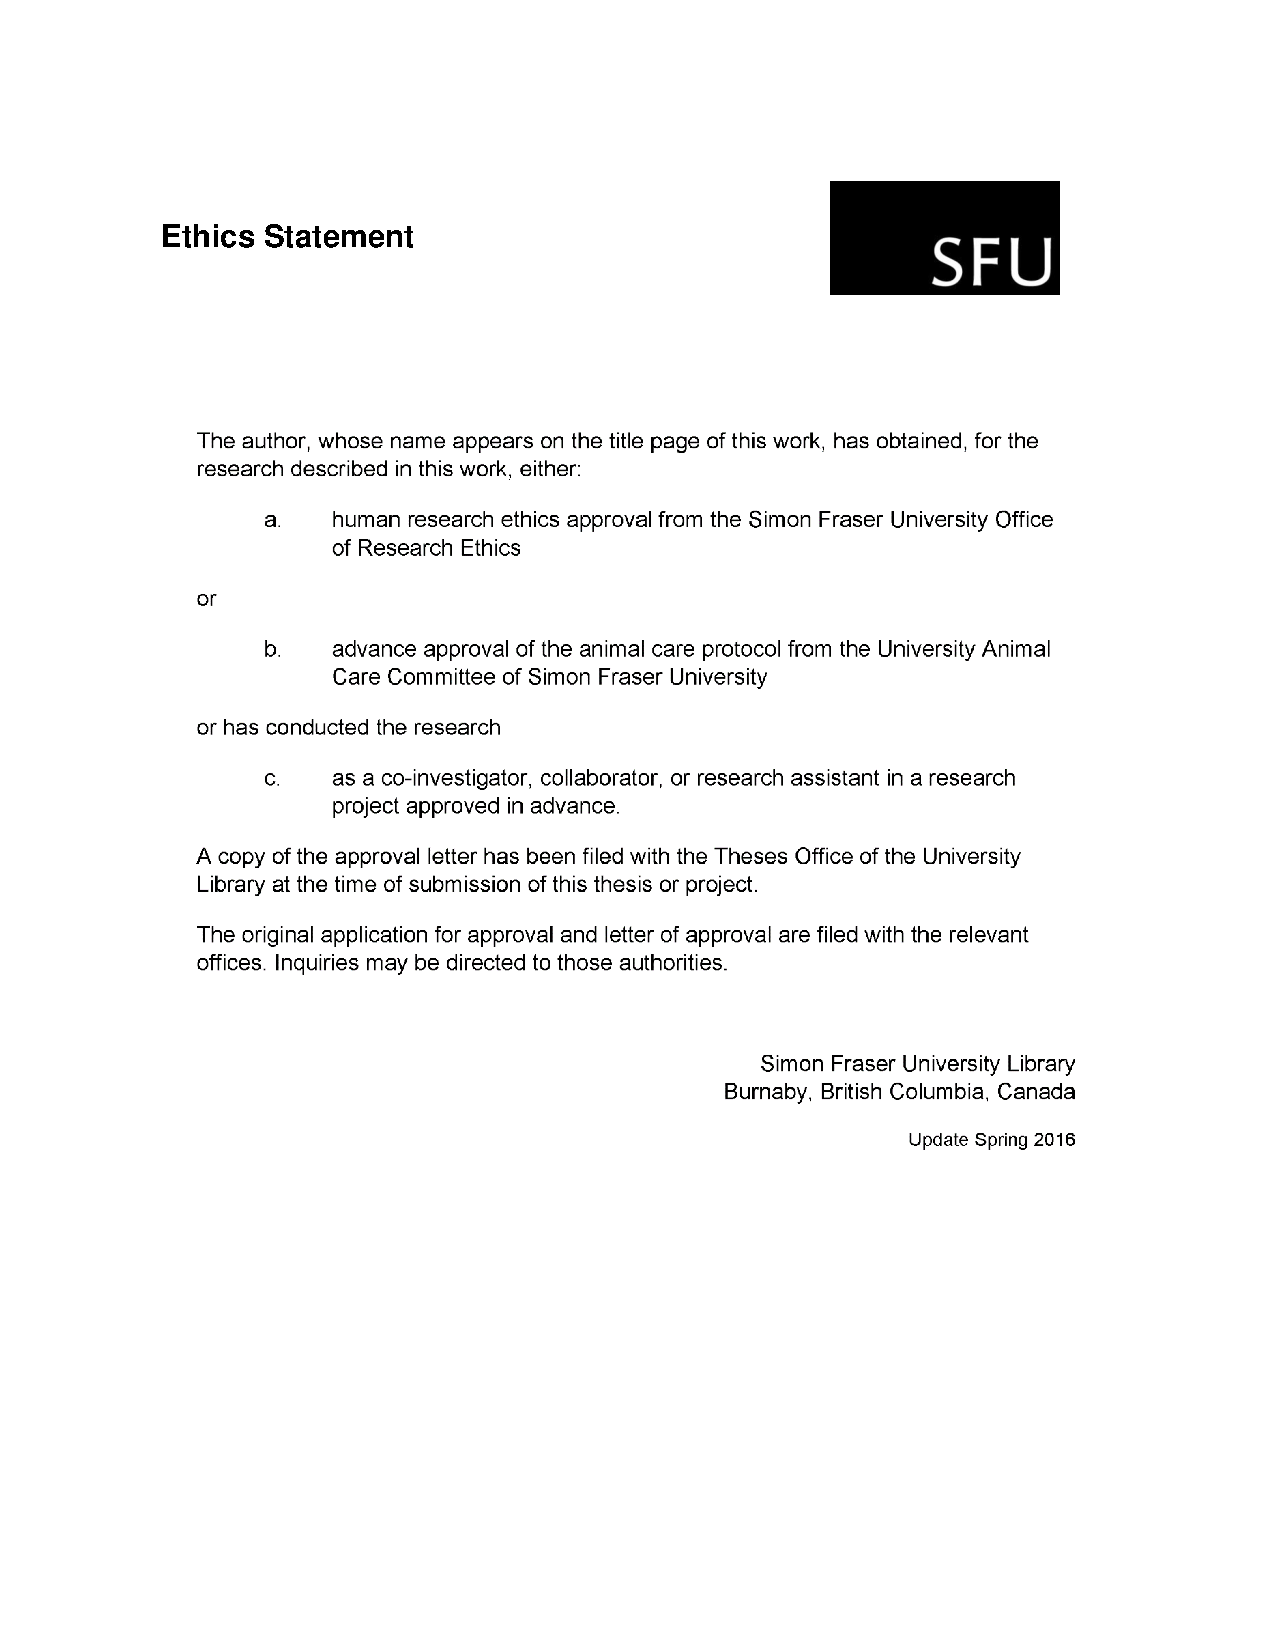
\includepdf[pagecommand={\thispagestyle{plain}}]{ethicsstatement.pdf}%
\clearpage

\begin{abstract}
	This is a blank document from which you can start writing your thesis.
\end{abstract}


\begin{dedication}
	This is an optional page.
\end{dedication}

\begin{acknowledgements}
	This is an optional page.
\end{acknowledgements}

\addtoToC{Table of Contents}%
\tableofcontents%
\clearpage

\addtoToC{List of Tables}%
\listoftables%
\clearpage

\addtoToC{List of Figures}%
\listoffigures%
\clearpage

\begin{preface}
I am the primary author of the work presented in this PhD dissertation. I was responsible for the design of experiments, data collection, data analysis and code, and manuscript preparation. Additional contributions for each chapter are described below.
\begin{flushleft}
\textbf{Chapter 1: Introduction}
\end{flushleft}
I am the primary author of this chapter, with intellectual contributions from L. B. Aknin and A. F. Shariff.
\begin{flushleft}
\textbf{Chapter 2: Cross-National Exploration of Attributions for Poverty and Support for Economic Inequality}
\end{flushleft}
A version of this chapter is currently under review at Nature Human Behavior. Wiwad, D., Piff, P. K., Robinson, A. R., Aknin, L. B., Mercier, B., \& Shariff, A. F. (2019). Inequality and the “self-made poor”: Motivating egalitarian behaviour by shifting attributions for poverty. I compiled, cleaned, and analyzed the data and prepared the manuscript. P. K. Piff co-wrote the manuscript. All additional authors provided intellectual contributions and edited the manuscript. 
\begin{flushleft}
\textbf{Chapter 3: Changing Situational Attributions for Poverty Through Perspective Taking}
\end{flushleft}
A version of this chapter is currently under review at Nature Human Behavior. Wiwad, D., Piff, P. K., Robinson, A. R., Aknin, L. B., Mercier, B., \& Shariff, A. F. (2019). Inequality and the “self-made poor”: Motivating egalitarian behaviour by shifting attributions for poverty. For the studies presented in this chapter and presented in the manuscript I compiled, cleaned, and analyzed the data, and prepared the manuscript. P. K. Piff co-drafted the manuscript. All additional authors provided intellectual contributions and edited the manuscript. 
\begin{flushleft}
\textbf{Chapter 4: Stereotype Disconfirmation and Cross-Socioeconomic Contact as a Means to Changing Attributions for Poverty}
\end{flushleft}
A version of this chapter will be submitted for publication. Wiwad, D., Shariff, A. F., \& Aknin, L. B. (In Prep). Addressing economic inequality through stereotype disconfirmation and cross-socioeconomic status contact. I designed the experiments, supervised data collection, and analyzed all data. L. B. Aknin and A. F. Shariff provided intellectual contributions and edited the manuscript.
\begin{flushleft}
\textbf{Chapter 5: Broad Causal Attributions}
\end{flushleft}
I designed the experiments, supervised data collection, conducted the analyses and prepared the manuscript. L. B. Aknin and A. F. Shariff provided intellectual contributions.
\begin{flushleft}
\textbf{Chapter 6: General Discussion}
\end{flushleft}
I am the primary author of this chapter, with intellectual contributions from L. B. Aknin and A. F. Shariff.
\end{preface}

%   MAIN MATTER  %%%%%%%%%%%%%%%%%%%%%%%%%%%%%%%%%%%%%%%%%%%%%%%%%%%%%%%%%%%%%%
%
%   Start writing your thesis --- or start \include ing chapters --- here.
%

\mainmatter%

\chapter{Introduction}

Economic inequality is defined as the wealth or income gap between the rich and the poor and has been labeled as one of the most pressing issues of the 21st century~\cite{obama13, piketty14, wilkinson17}. Stark examples of inequality abound: the top ten Forbes’ billionaires own more wealth than the GDP of some countries (e.g., Nigeria, Belgium, and the United Arab Emirates), the median wealth of the top 5\% of U.S. households surpasses the wealth of the median household by a factor of 90~\cite{inequalityorg17}, and the top 1\% of earners in the United States command the same amount of wealth as the bottom 90\%~\cite{Wolff10}. Many academics have argued that economic inequality is not a benign economic indicator, but instead plays a substantial role shaping the fabric of a society, often leading to undesirable psychological~\cite{wilkinson06b, wilkinson06} and political consequences~\cite{murphy01}. For example, cities and nations with higher economic inequality tend to display higher social unrest~\cite{lichbach89}, lower social trust and higher mortality~\cite{kawachi97}, higher rates of violent crime~\cite{wilson97}, worse health~\cite{wilkinson06}, and stifled economic growth~\cite{persson94}.

Despite these significant costs, inequality ranks disproportionately low as an issue of concern in some countries. For example, a 2016 Gallup poll conducted in the United States revealed that the gap between the rich and the poor ranked a distant 12th among people’s chief concerns, behind issues such as terrorism, immigration, and general dissatisfaction with the government – issues that are arguably less of an immediate threat to the country than economic inequality~\cite{mccarthy16}. Why? While there are likely a multitude of reasons, one possibility may be that people misperceive the level of economic inequality in the United States. Supporting this possibility, Kiatpongsan and Norton~\cite{kiatpongsan14} found that a large sample of Americans estimated the gap in yearly earnings between the average CEO and average worker was 30:1 when in reality the gap was 354:1. That is, for every \$1 the average worker earns, a CEO earns, on average, \$354. These data show that the average citizen underestimates the extent of wage inequality by a factor of 12, it is thus unsurprising that economic inequality ranks disproportionately low as a concern in the United States.

Another reason that people may be relatively apathetic to economic inequality is that people view poverty, wealth, and socioeconomic status as deserved as opposed to at least, in part, due to outside factors, such as luck or systemic injustices. Indeed, a large body of past research has shown that North Americans tend to make dispositional attributions for others’ behaviour and outcomes~\cite{miller84, morris94}, including poverty~\cite{bullock95, cozzarelli01, feather74, halpern93}. Holding dispositional attributions for socioeconomic status may impact evaluations towards economic inequality and help directed toward the poor. Supporting this possibility, past research has shown that individuals holding strong dispositional attributions for poverty tend to experience greater blame and anger towards the poor~\cite{cozzarelli01, zucker93}, as well as support more restrictive welfare policies~\cite{bullock03}. Meanwhile, individuals who hold strong situational attributions for poverty report greater willingness to help the poor~\cite{bullock03} and support for more progressive social welfare programs~\cite{kluegel86}. Building upon this work, my dissertation will focus on understanding the causal link between attributions for poverty and attitudes and behaviour aimed at mitigating economic inequality. 

\section{Attribution Theory}

As a species, humans are fascinated with causality; we appear to have an inherent desire to understand the causes of everything from the vastness of space to why someone chooses a certain dish at a restaurant~\cite{ariely00, weiner85}. One perspective on this obsession suggests that we are motivated to understand causality as a tool to master our environment~\cite{white59}. That is, we have an inherent desire to understand how the world around us functions in order to behave and interact with this environment. Building on this inherent desire for mastery, mastering our environment via understanding the causes of behavior is both practical and functional; when we achieve a desired outcome, we want to understand its cause(s) so we can repeat the success~\cite{kelley73}. Conversely, when we fail to achieve a desired outcome we want to understand why to ensure that failure never happens again. Researchers have been exploring how we understand causality, and how we make mistakes understanding causality, since Lewin~\cite{lewin35} first observed a general over-reliance on explaining behaviour in terms of internal states. Heider~\cite{heider58} then laid the ground work for what would become decades of research outlining Attribution Theory.

Heider~\cite{heider58} pioneered the emergence of attribution theories via the development of his Social Perception Theory. While not directly an attribution theory per se, Heider~\cite{heider58} presented two key insights that directly influenced the development of subsequent theories. First, Heider~\cite{heider58} suggested that the way we perceive other peoples’ behaviour is analogous to the way we perceive objects and can therefore be influenced by context. For instance, the phenomena of scent habituation~\cite{pellegrino17}. The smell of a Thanksgiving dinner being prepared is almost overwhelming when one first enters the house on the holiday but is nearly undetectable after a small amount of time despite the sensory input remaining identical—perception changes with context. Heider~\cite{heider58} argued that social perception functions much the same way as physical perception—the contextual lens can influence the way we understand and interpret a behaviour. From this, Heider~\cite{heider58} purported that social perceptions are susceptible to errors and biases (i.e., underestimating the situational influences on human outcomes) in much the same way that physical perceptions are (i.e., optical illusions).

Heider’s~\cite{heider58} second, and arguably more important, insight was the idea that both internal/dispositional and external/situational factors play substantial roles in determining human behaviour. Dispositional causes refer to any perceived cause of a particular behaviour that is inside the actor (e.g., their personality, genes), whereas situational causes refer to any perceived cause that is outside the actor (e.g., another person, bad luck, etc). Heider (1958) proposed that when making causal attributions for an actor’s behaviour (e.g., bad spending habits) or outcomes (e.g., living in poverty), we can attribute said behaviour or outcome to dispositional or situational causes. Combining his two key ideas, Heider~\cite{heider58} proposed that social perceptions often suffer from a common error – people tend to underestimate the impact of situational causes of behaviour when making attributions. This phenomenon was formalized decades later as the “Fundamental Attribution Error”~\cite{ross77}.

Heider’s~\cite{heider58} ideas regarding errors in social perception, and the distinction between dispositional and situational attributions, paved the path for numerous theoretical advances in understanding how and when we make causal attributions~\cite{bem72, jones65, kelley67, kruglanski75, weiner85}. The first large step in formalizing a theory of attributional processes was Correspondent Inference Theory (CIT;~\cite{jones65}). CIT was built directly on Heider’s~\cite{heider58} Social Perception Theory and was one of the first explorations into how an observer ultimately decides whether or not internal factors caused another person’s behaviour. In their basic model, Jones and Davis~\cite{jones65} suggested that an observer looks at two pieces of information when attempting to determine the causes of an action: was the actor’s behaviour (a) intentional, and (b) socially undesirable? According to their model, an observer is most likely to make dispositional/correspondent attributions (i.e., believe that the actor’s behaviour corresponds to their internal state) when the behaviour appears intentional and is socially undesirable. If a person has little to gain from their actions (e.g., by being rude at a party), it is likely that the behaviour reflects their disposition, indicating that they are a rude person. However, if a person stands to gain social rewards (e.g., by being exceptionally nice at a party), we cannot make dispositional inferences because we do not know if the person was acting that way because of their internal state (i.e., they are a nice person) or simply to gain a personal benefit (e.g., social favor). Here, the context of the behaviour (i.e., a party) is shaping how we determine the internal or external nature of the actor’s behaviour.

Weiner~\cite{weiner85} then consolidated Jones and Davis’~\cite{jones65} theoretical ideas regarding causal attributions into the first formal “Attribution Theory” highlighting three components of causal attribution: locus, controllability, and stability. Locus refers to whether the cause of behaviour is located within (internal) or outside (external) of the actor (e.g., a personality trait or luck). Controllability refers to what degree the actor can control the behaviour (e.g., choosing to buy an apple is controllable, slipping on ice may not be). Finally, stability refers to how consistent the behaviour is over time (e.g., does she always choose to buy an apple when looking for a snack?). This work on causal attributions brought to light nuances in the way we understand the causes of our own and other’s behaviour. The way that a given person determines whether a behaviour or outcome is internal/external, controllable, and stable is not universal. In particular, there are strong cultural differences in the development of attributional styles.

A body of cross-cultural research (See~\cite{smith93} for a review) following Weiner’s~\cite{weiner85} Attribution Theory shed light on how people develop an attributional style.  Specifically, how in Western societies an individual often comes to rely predominantly on dispositional attributions for a behaviour, often ignoring the “power of the situation” (i.e., how strongly situational factors can influence behaviour). Past research demonstrates that there are predictable cultural differences in general attribution styles between individualistic and collectivistic societies. People raised in individualistic countries, such as the United States, tend to make predominantly dispositional attributions for others’ behaviour relative to people raised in collectivistic countries, such as China or Finland (~\cite{lee96, miller84,morris94}; see~\cite{smith93} for a review). For example, Lee and colleagues~\cite{lee96} compared the language of newspaper articles written in China and the United States and found that American newspapers more frequently made dispositional attributions for behaviour. Morris and Peng~\cite{morris94} additionally showed that in explaining the causes of recent murders, American survey respondents, as opposed to Chinese survey respondents, favored more dispositional explanations, such as mental instability and personality problems.

Importantly, these cultural differences in attribution are not innate. That is, attributional styles are shaped by the culture people live in and are thus malleable. Indeed, research indicates that these cultural differences emerge in part through distinct socialization patterns; people learn attributional styles from their parents and peers. If these cultural differences were innate, as opposed to socialized, there would be minimal variation within a culture, which is not the case~\cite{smith93}. Supporting this socialization theory, researchers have shown that simply imagining oneself as a distinct individual or as part of a collectivist group changes their attributional style. For instance, Trafimow, Triandis, and Goto~\cite{trafimow91} had a small sample of North American and Chinese undergraduates spend ten minutes thinking of ways they are either similar or different to their family to prime a collectivistic/interdependent versus individualistic/independent mindset before asking questions to assess attributional style. Regardless of their cultural background, participants randomly assigned to the individualistic mindset condition via thinking about their differences from others were more prone to making dispositional attributions. With respect to the present research, the key implication from these studies is that they suggest that attributional styles are malleable. Simply having one think about themselves in individual or collective way can shift attributional style. Thus, it may be possible to introduce interventions that shift attributional style.

In addition to attributional styles appearing malleable, some theoretical and empirical work suggests that dispositional and situational attributions are also orthogonal. Theoretically, Kluegel and Smith~\cite{kluegel86} argued that people judge the causes of behaviour using the easiest to access, top-of-mind, information. Therefore, presenting someone with information regarding the situational causes of poverty may simply bring situational factors to the forefront while leaving an individual’s underlying dispositional attributions for poverty unchanged. Empirically, past work has lent support to this idea, showing that dispositional and situational attributions for behaviour are roughly uncorrelated, as opposed to negatively correlated as one might expect if they were not orthogonal~\cite{taylor76, miller81}. Given that attributional styles appear to be malleable and influenced by salience heuristics, it seems plausible that our perceptions of the causes of behaviour are not necessarily an accurate representation of reality. In what ways are causal attributions biased, and can we address these biases?

\section{Biases in the Attribution Process and Attributions for Poverty}

A large body of research demonstrates that individuals in Western society often make dispositional attributions for others’ behaviour and overlook the impact of situational determinants in shaping behaviour. This bias is so pervasive in Western culture (e.g., see~\cite{morris94} for a review) that it has been labeled the “Fundamental Attribution Error" (FAE;~\cite{ross77}). Numerous experiments have demonstrated the FAE in action. For instance, in the classic FAE study, a group of students were randomly assigned to write and read aloud an essay that was pro-Castro and another group of students were assigned to write and read aloud an essay that was anti-Castro. Students who listened to the essay were asked to predict whether the essay writer was in favor or opposed to Castro. Consistent with the FAE, listeners assumed that writers who wrote and read pro-Castro essays were for Castro while those who wrote and read anti-Castro essays were against Castro. Critically, however, when researchers informed participants that the essay writer’s stance (pro or anti) was determined by the experimenter, participants continued to erroneously believe that the stance of the essay reflected the beliefs of the essay writer, albeit to a slightly smaller degree~\cite{jones67}. Here, the FAE manifests in the fact that the observers defaulted to making internal attributions and failed to correct their attributions, despite being shown clear evidence to the contrary.

An over-reliance on dispositional explanations for other’s behaviour and outcomes (e.g., the FAE) can influence the way that we think about and treat various social groups, a phenomenon known as the Ultimate Attribution Error (UAE;~\cite{pettigrew79}). The UAE is a group-level application of the FAE that often leads people to attribute an outgroup members’ unfavorable outcomes to internal factors and favourable outcomes to chance. For instance, an outgroup observer may believe that someone is poor because they are lazy or incompetent despite the fact that poverty may be caused by numerous situational factors, such as high unemployment rates (e.g.,~\cite{krohn76}), stagnating wages~\cite{desilver14}, unexpected and uncontrollable illness (e.g.,~\cite{grau88}), predatory lending practices (e.g.,~\cite{engel02}), and constant cognitive load (e.g.,~\cite{mani13}). Indeed, people in Western societies rely predominantly on internal attributions for poverty~\cite{cozzarelli01, feather74}. Demonstrating this, Feather~\cite{feather74} examined a community sample of Australians and found that the majority of respondents attributed poverty to internal factors, such as lack of thrift and poor money management, while simultaneously minimizing external factors, such as bad luck. Additionally, Feather~\cite{feather74} found that Americans were more likely than Australians to endorse dispositional factors consistent with the Protestant Work Ethic (e.g., “loose morals,” lack of effort, and drunkenness) when explaining the causes of poverty. Cozzarelli and colleagues~\cite{cozzarelli01} corroborated these findings in a sample of Midwestern college students, demonstrating that respondents were most likely to make dispositional attributions for poverty.

The tendency to make dispositional attributions for poverty may impede a willingness to address inequality. There are myriad ways to address inequality. Inequality could be dampened with bottom-up or top-down approaches by, for example, providing support to the poor or more heavily taxing the rich. While beliefs about inequality and poverty are difficult to untangle, in this dissertation I will focus predominantly on willingness to help the poor as an avenue for addressing growing inequality. Broadly speaking, past research on the belief in a just world has shown that when someone views the world as just, they are less willing to help, and more willing to blame victims~\cite{correia01}. More directly, Furnham and Gunter~\cite{furnham84} found that people who demonstrated a stronger belief in a just world endorsed more negative views of people who live in poverty; for example, the belief that people in poverty are lazy, deserving of their economic station, and unpleasant. These studies suggest that dispositional explanations for poverty may preclude action aimed at challenging economic inequality by helping the poor. When one views the poor as deserving of their economic station, they may be less willing to help or endorse government policies aimed at helping them.

Despite the myriad of past studies demonstrating that North Americans make predominantly dispositional attributions for poverty, no prior research has explored the malleability of attributions for poverty or explored whether shifting these attributions can impact economic attitudes and behaviours. As I have discussed thus far, attributional styles seem to be malleable. Therefore, in the remainder of this dissertation I will (1) explore how attributions for poverty relate to support for economic inequality, and (2) investigate the efficacy and outcomes of shifting attributions for poverty on support for economic inequality.

\section{Dissertation Overview}

Past research has demonstrated that North Americans tend to rely on dispositional attributions when explaining the behaviour of others, while simultaneously overlooking the power of the situation. This tendency occurs when making attributions about people in many domains and, critically for this this dissertation, is frequently applied to individuals who live in poverty. For instance, in the United States, most people blame the poor for living below the poverty line (e.g.,~\cite{feather74, cozzarelli01}) and minimal consideration is given to the various situational causes of poverty~\cite{davidai16}. In six studies, I used various methodologies (analysis of large-scale cross-national data, high-powered pre-registered laboratory experiments, and a quasi-experimental field study) to explore how causal attributions for poverty and behaviour more generally are linked to and causally influence attitudes towards economic inequality. Additionally, I sought to explore whether reducing reliance on dispositional attributions and increasing knowledge of the power of the situation can change perceptions of the poor and beliefs about economic inequality.

Previous research has demonstrated a link between attributions for poverty, support for economic inequality, and attitudes towards the poor~\cite{bullock03, cozzarelli01, kluegel86, zucker93}. Generally, this work was conducted with small sample sizes (ns < 200) and therefore presents limited generalizability. Kluegel and Smith~\cite{kluegel86} was a more comprehensive set of national surveys but was still conducted only within the United States. Thus, in Study 1 I conducted a world-wide assessment exploring whether attributions for poverty are related to support for economic inequality utilizing a large-scale cross-national sample of 34 countries. Here, I attempted to present more definitive and concrete evidence that causal attributions are related to beliefs about inequality around the globe.

Building upon evidence of an association between attributions for poverty and support for economic inequality using world-wide data, I sought to examine the causal nature of this relationship. First, in Studies 2a and 2b I conducted a set of experimental tests aimed at increasing situational attributions for poverty. In a small-scale experiment, as well as a high-powered pre-registered replication, I examined whether situational attributions for poverty are causally linked to attitudes towards economic inequality. I tested this link by having participants engage in a computer game that promotes perspective taking and provides information regarding the external challenges that come with living in poverty to increases situational attributions for poverty (relative to a neutral control condition) and explore subsequent differences in attitudes towards economic inequality. In Study 2b, along with the larger sample, I made several design improvements to strengthen the causal conclusions. 

In Studies 3a and 3b I conducted another set of experimental tests, this time aimed at examining whether dispositional attributions for poverty are causally linked to attitudes towards economic inequality. In another small-scale experiment, and high-powered pre-registered replication, I examined whether a strong instance of stereotype inconsistency presented through a cross-socioeconomic status interaction reduced dispositional attributions for poverty and explored subsequent changes in attitudes towards economic inequality. As with the previous studies, I made several design changes to Study 3b in order to address limitations with Study 3a.

Lastly, in Study 4 I took this exploration out of the lab and into the field. The main goal of Study 4 was to explore whether we see changes in attributions for poverty when students learn about the situational causes of behaviour (more broadly) in a general classroom setting. I followed students over two semesters who were taking an introductory social psychology class that regularly discusses the power of the situation, compared with various control classes that did not have the same focus. I examined whether learning about the situational causes of behavior more broadly, as opposed to just poverty, in a natural learning environment would have a meaningful effect on downstream attitudes about poverty and economic inequality. 
The six studies presented in this dissertation form the first, to my knowledge, test of whether we can shift attributions for poverty via various interventions such as a poverty simulation, cross-socioeconomic status contact, and learning about “the power of the situation” in a classroom setting. More crucially, these studies are the first to experimentally link attributions for poverty with various psychological attitudes such as support for inequality and redistribution, as well as behaviours such as willingness to help the poor.


\chapter{Cross-National Exploration of Attributions for Poverty and Support for Economic Inequality}

There are myriad situational factors that determine whether or not someone is living in poverty~\cite{piff18}. These factors include high unemployment and stagnating wages~\cite{desilver14}, uncontrollable illness (e.g.,~\cite{grau88}), predatory lending (e.g.,~\cite{engel02}), and chronic cognitive load (e.g.,~\cite{mani13}). Despite these environmental determinants, people in the United States predominantly explain poverty as caused by internal traits or dispositions such as laziness, poor planning, or a lack of self-control (e.g.,~\cite{cozzarelli01, feagin75, feather74, halpern93}).

Importantly, attributions for poverty are related to various attitudes towards the poor and policies aimed at helping them. For instance, dispositional attributions for poverty are correlated with blame and anger toward the poor, reduced support for helping them~\cite{cozzarelli01, zucker93}, and increased support for restrictive social welfare policies~\cite{bullock03}. On the other hand, situational attributions for poverty correlate with increased personal sympathy for and willingness to help the poor~\cite{osborne15, zucker93}, and greater support for progressive welfare programs that aid them––for example via increasing funding for healthcare~\cite{bullock03, kluegel86}.

Beyond the influence of attributions for poverty on beliefs about the poor specifically, another important avenue to explore is how these attributions inform attitudes about systemic conditions (e.g., economic inequality). Guided by the past research connecting attributions for poverty and beliefs about the poor, I theorized that a strong reliance on dispositional (as opposed to situational) attributions for poverty would be related to greater support for the current level of economic inequality. Specifically, in this initial exploration I sought to explore how attributions for poverty relate to support for economic inequality cross-nationally. It stands to reason that if people believe the poor are poor because they are lazy or lack self-control, people may see wealth disparities as fair and just—people rise, or fall, to the economic station they deserve, thus wealth disparity is reasonable and fair. However, if people believe the poor are poor due to external and uncontrollable factors, people may see wealth disparities as unfair and unjust.

In this chapter I present an initial cross-national exploration of the hypothesis that situational (as opposed to dispositional) attributions for poverty are associated with lower support for economic inequality. All data and R code for cleaning, preparing, and analyzing these data can be found at this \href{https://github.com/dwiwad/Dissertation/tree/master/Study\%201}{Github repository for Study 1}.

\section{Study 1: Cross-national exploration of the link between attributions for poverty and support for economic inequality}

\subsection{Data}

\subsubsection{Participants} 
I combined individual level data from the 1995-1998 wave of the World Values Survey (WVS;~\cite{inglehart}) and country level data from the International Social Survey Programme’s~\cite{issp09} survey on social inequality. This diverse initial sample of 77,129 (Median age = 35-44, 50.5\% Male) WVS respondents was spread across 54 countries (Figure \ref{fig:firstfig}). 

\begin{figure}[h]
  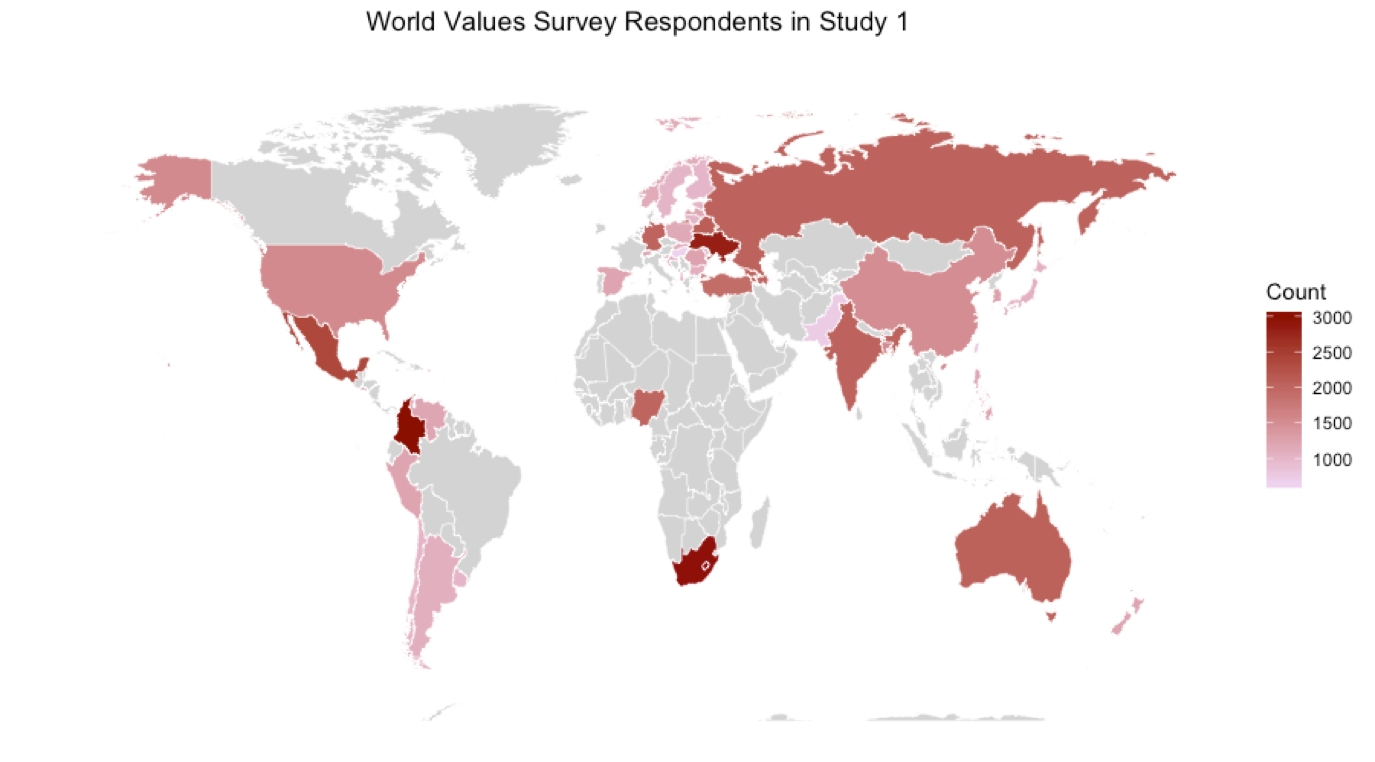
\includegraphics[width=\linewidth]{Fig2-1.png}
  \caption{World Values Survey Number of Respondents by Country}
  \label{fig:firstfig}
\end{figure}

\subsubsection{Individual-Level Measures from the World Values Survey}
I utilized two key individual measures from the World Values Survey~\cite{inglehart}--attributions for poverty and support for economic inequality--as well as several demographic covariates. The descriptive statistics reported below reflect the final individual sample (n = 40,031); I will reserve discussion of my handling of missing data until after describing the measures.

\subparagraph{Attributions for Poverty.} Respondents reported their attributions for poverty by choosing one of two responses to the WVS question “why, in your opinion, are there people in this country who live in need” (1 = “people are poor because of an unfair society” or 2 = “people are poor due to laziness or lack of willpower”). Approximately two and half times as many respondents endorsed laziness or a lack of willpower (i.e., dispositional attribution), as opposed to the unfair society (i.e., situational attribution), as the dominant cause of poverty (n\textsubscript{lazy} = 28,291, n\textsubscript{society} = 11,740 ; $\chi$\textsuperscript{2}(1) = 6843.1, \textit{p} < .001). 

\subparagraph{Support for Economic Inequality.} Respondents reported their support for economic inequality (\textit{M} = 5.94, \textit{SD} = 2.95) by responding to the prompt “Now I’d like you to tell me about your views on various issues. How would you place your views on this scale? 1 means you completely agree with the statement on the left; 10 means you completely agree with the statement on the right; and if your views fall somewhere in between, you can choose any number in between.” Respondents positioned themselves on a ten-point scale ranging from 1 (“Incomes should be made more equal”) to 10 (“We need larger income differences to act as incentives for individual effort”).

\subparagraph{Covariates.} I included four relevant individual-level covariates from the World Values Survey: Religiosity, Political ideology, Education, and Income. First, respondents reported their religiosity by answering the question “how important is [religion] in your life” on a four-point scale ranging from 1 (“very important”) to 4 (“not at all important;” \textit{M} = 2.10, \textit{SD} = 1.06). Second, respondents reported their political ideology on a single item (“In political matters, people talk of ‘the left’ and ‘the right.’ How would you place your views on this scale, generally speaking?”) on a 1 (“Left”) to 10 (“Right) scale (\textit{M} = 5.79, \textit{SD} = 2.98). Third, respondents reported their broad level of education on a nine-point scale ranging from 1 (“No formal education”) to 9 (“University level education; with degree”; \textit{Median} = 5: Completed Secondary School; Technical/Vocational Type, \textit{SD} = 2.22). Lastly, respondents reported their income on a ten-point country-specific income ladder (\textit{Median} = 4th decile, \textit{SD} = 2.52). Specifically, participants were asked “we would like to know in what group your household income is, counting all wages, salaries, pensions, and other income. Just give the [number] of the group your household falls into, before taxes and other deductions.” Additionally, participants reported their age and gender.

\subsubsection{Country-level Measures}
I acquired country level data from 34 countries from The World Bank~\cite{worldbank14, worldbank15} in order to account for important country level covariates. Specifically, I included the Gini Coefficient (\textit{M} = .41, \textit{SD} = .11) and GDP per capita (\textit{M} = 6,777.46, \textit{SD} = 9506.84) from The World Bank~\cite{worldbank14, worldbank15}. In order to keep the data consistent with the World Values Survey, I used Gini and GDP per capita data from 1995 when available. If I was unable to find these data, I used figures up to and including 1998. 

\subsection{Missing Data and Participant Exclusions}

In the initial data set there was a total sample of 77,129 individuals across 45 countries. As is typical in large datasets, there were missing data on every key variable: support for economic inequality (n\textsubscript{miss} = 6,381), attributions for poverty (n\textsubscript{miss} = 14,518), political ideology (n\textsubscript{miss} = 20,705), age (n\textsubscript{miss} = 179), gender (n\textsubscript{miss} = 76), education (n\textsubscript{miss} = 2,877), income (n\textsubscript{miss} = 10,311), and religiosity (n\textsubscript{miss} = 2,779).\footnote{Often, missing data presents a challenge in that a study can become underpowered when a researcher removes respondents with missing data. However, in this case, the sample size was large enough that a significant decrease in statistical power due to participant loss is not a primary concern; as such my focus on handling the missing data was to choose a strategy that would introduce the least bias into the analyses. If the data are “Missing Completely at Random” (MCAR) simple listwise deletion will not introduce any bias. However, if the data are not MCAR, listwise deletion will likely introduce bias (e.g., perhaps respondents who choose not to answer a certain question share a psychological trait that is now being excluded from the data) and thus multiple imputation is often the preferred method~\cite{he11}. However, listwise deletion can often be the least biased method even if the data are not MCAR, especially when the data set is large enough that we are not worried about a drop in statistical power from list wise deletion~\cite{allison09}. This is, in part, because in a large data set utilizing multiple imputation can result in imputing tens of thousands of non-existent data points.}  

Within the WVS missing data is classified in one of five ways: (1) missing; unknown, (2) not asked in survey, (3) not applicable, (4) no answer, or (5) don’t know. In this particular wave (1995-1998), all missing data was either “not asked in survey,” or the respondent gave no answer/did not know. I found that almost all missing data that was not asked in the survey was clustered by country. For instance, the question regarding attributions for poverty simply was not asked in Switzerland. I used listwise deletion to remove all responses that were missing because they were not asked in the survey. While these responses were clustered under country, and thus by definition not MCAR, listwise deletion was likely to introduce less bias than imputation precisely due to the country-level clustering.\footnote{I did, however, investigate the assumption of MCAR using Little’s~\cite{little81} test which I implemented using the BaylorEdPsych package~\cite{baylor} in R~\cite{rcore}. In Little’s~\cite{little81} test, the null distribution is an asymptotic chi-square distribution where failure to reject the null hypothesis suggests that the data are MCAR. I found that the missing values in our target variables were not MCAR, $\chi$\textsuperscript{2}(425) = 3500.66, \textit{p} < .001. However, chi-square tests are highly sensitive to sample size making this assessment difficult to interpret--with a sample size as large as nearly 65,000 I was liable to falsely reject the null hypothesis of MCAR for potentially insignificant deviations from the null distribution. Additionally, as a logic check, I ran a multiple mean-imputation using the mice package~\cite{vanbuuren11} in R~\cite{rcore}. The pooled results of five separate mean imputations produced nearly identical coefficients to the analysis of the list wise deleted data. Therefore, I am confident in the decision to not impute and subsequently analyze over 20,000 data points. See the \href{https://github.com/dwiwad/Dissertation/blob/master/Study\%201}{Study 1 R analysis file} for complete analyses.} For example, using the scores on support for inequality in the United States to impute scores on support for inequality in China would surely lead to biased estimates as there are significant cultural differences between the two countries. The sample size after removing participants who were not asked key questions was 64,072 (See \href{http://github.com/dwiwad/Dissertation/blob/master/Study 1/Study_1.pdf}{R analysis file} for full missing data analysis). Following this, given that listwise deletion is likely to be the least biased method for handling missing data in a large data set, I opted to remove all rows with missing data on any variable resulting in a complete-cases individual data set of 40,031 observations. 

\subsection{Results}
\subsubsection{Individual-Level Analysis}

To examine whether attributions for poverty are related to support for economic inequality I first regressed support for economic inequality on to attributions for poverty for the full sample of 40,031 respondents.  In line with my prediction, I detected a small effect indicating that survey respondents who made more situational attributions for poverty also reported reduced support for economic inequality ($\beta$ = -0.07, \textit{p} < .001). Importantly, this finding held ($\beta$ = -0.06, \textit{p} < .001) when controlling for political ideology, income, religiosity, education, age, and gender (Table \ref{tab:firsttable}). 

\begin{table}[h]
  \begin{center}
    \caption{Summary of the regression analysis for variables predicting attitudes towards economic inequality (n = 40,031)}
    \label{tab:firsttable}
    \begin{tabular}{l c c c r}% <-- Alignments: 1st column left, 2nd middle and 3rd right, with no vertical lines in between
    \hline
       & $\beta$ & Std. Error & \textit{t} & \multicolumn{1}{c}{\textit{p}}\\
       \hline
       Intercept & \multicolumn{1}{S}{.00} & .005 & \multicolumn{1}{S}{.00} & .999\\
       Attributions for Poverty & \multicolumn{1}{S}{-.057} & .005 & \multicolumn{1}{S}{-11.581} & < .001\\
       Political Ideology & \multicolumn{1}{S}{.120} & .005 & \multicolumn{1}{S}{24.275} & < .001\\
       Education & \multicolumn{1}{S}{.133} & .005 & \multicolumn{1}{S}{25.313} & < .001\\
       Income & \multicolumn{1}{S}{.038} & .005 & \multicolumn{1}{S}{7.372} & < .001\\
       Religiosity & \multicolumn{1}{S}{-.024} & .005 & \multicolumn{1}{S}{-4.909} & < .001\\
       Age & \multicolumn{1}{S}{-.012} & .005 & \multicolumn{1}{S}{-2.462} & . 014\\
       Gender & \multicolumn{1}{S}{-.009} & .005 & \multicolumn{1}{S}{-1.850} & .063\\
       \hline
    \end{tabular}
  \end{center}
\end{table}

While these effects are relatively small, the density of support for economic inequality demonstrates a clear pattern of responding between people who reported dispositional (versus situational) attributions for poverty (Figure \ref{fig:secondfig}). The respondents who endorsed dispositional explanations for poverty are far more clustered on the “wanting larger income differences” end of the distribution than are respondents who endorsed situational explanations for poverty.

\begin{figure}[h]
  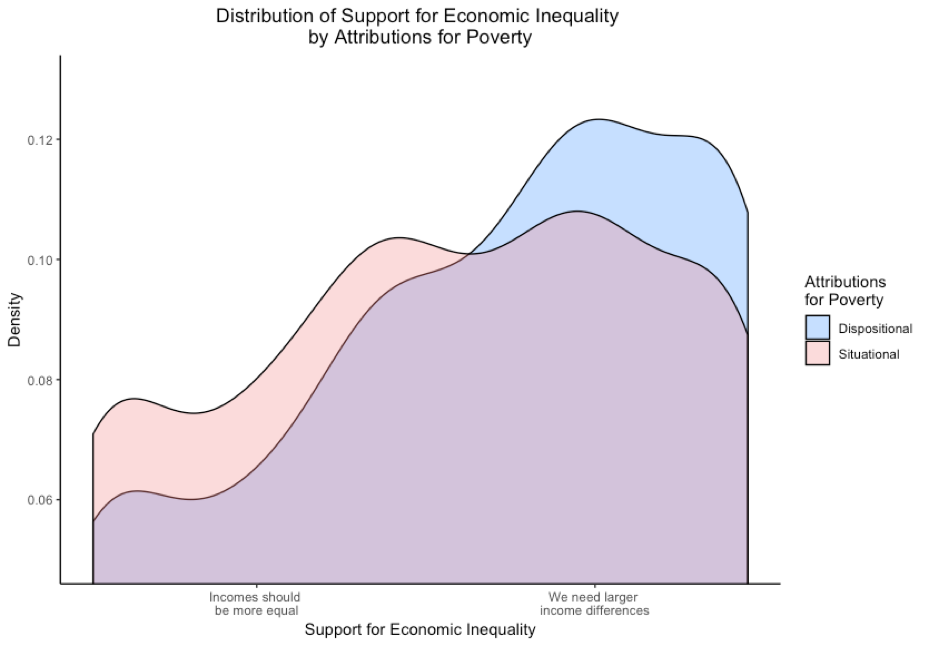
\includegraphics[width=\linewidth]{Fig2-2.png}
  \caption{Response patterns on "support for economic inequality" for survey respondents reporting dispositional (versus situational) attributions for poverty}
  \label{fig:secondfig}
\end{figure}

While this individual-level analysis provides initial support for the hypothesis that endorsement of situational (as opposed to dispositional) attributions for poverty is related to decreased support for economic inequality, this analysis was limited in that it does not allow us to consider the relative level of wealth and inequality where each respondent lives. For instance, beliefs about the acceptability of inequality are likely to be different between participants who live in highly equal societies, such as Norway, relative to highly unequal societies, such as South Africa. As such, I conducted a cross-national multilevel model, which provided a more powerful analysis at the individual level while accounting for within-country clustering on the dependent variable. 

\subsubsection{Multilevel Model}
In order to determine if there is significant country-level clustering in the data, I quantified and compared how much variance in support for economic inequality is occurring between and within countries. That is, is there more similarity in support for economic inequality within each country than there is between countries? If this is indeed the case, it would suggest that the country in which one lives is influencing support for economic inequality in some way and thus the data are not independent—a critical assumption in linear regression. The Intraclass Correlation Coefficient (ICC) directly tests this assumption by comparing the within and between group variance in a dependent variable~\cite{killip04}. To calculate the ICC I ran an unconditional random analysis of variance (the “null model”), entering only the grouping variable (country) and the outcome variable, support for economic inequality, into Model 1 (Table \ref{tab:secondtable}). As is typical, I found that far less of the variance on support for economic inequality was explained between countries (\textit{s}\textsuperscript{2} = .082) than within countries (\textit{s}\textsuperscript{2} = .920). At first blush this shows that support for economic inequality is being predominantly determined at the individual level, with only a small amount of variance being explained by group (i.e., country-level) differences. In using these variances to calculate the ICC (i.e., the proportion of the total variance explained that is stemming from group differences), I found that the country in which one lives explains approximately 8\% (ICC = 0.08) of the total variance, suggesting that there is some degree of scores on support for economic inequality are stemming from group differences. 

While there is no hard and fast rule, multilevel modeling rules of thumb suggest that 8\% is enough within-country clustering of the dependent variable to significantly inflate type I error rates~\cite{killip04}. Thus, I decided to move forward with conducting follow up multilevel models to account for this within country clustering. One added benefit of conducting a multilevel model in this context is the ability to control for country level predictors that would be reasonable expected to influence support for economic inequality. Specifically, in this case, a multilevel model allows me to control for the actual level of economic inequality as well as Gross Domestic Product (GDP) per capita in a given country.

\begin{table}[h]
  \begin{center}
    \caption{Summary of the multilevel regression analysis predicting attitudes towards economic inequality}
    \label{tab:secondtable}
    \begin{tabular}{l c c c c c c}% <-- Alignments: 1st column left, 2nd middle and 3rd right, with no vertical lines in between
    \hline   
       & \multicolumn{2}{c}{\textbf{Model 1:}} & \multicolumn{2}{c}{\textbf{Model 2: Atts.}} & \multicolumn{2}{c}{\textbf{Model 3:}}\\
       & \multicolumn{2}{c}{\textbf{Null Model}} & \multicolumn{2}{c}{\textbf{for Poverty Only}} & \multicolumn{2}{c}{\textbf{Full Model}}\\
       & $\beta$ & SE & $\beta$ & SE & $\beta$ & SE\\
      \hline
      Intercept ($\gamma$\textsubscript{00}) & -0.009 & 0.043 & \multicolumn{1}{S}{-0.010} & \multicolumn{1}{S}{0.043} & \multicolumn{1}{S}{-0.011} & \multicolumn{1}{S}{0.056}\\
     \textbf{Fixed Effects}\\
      \underline{Level 1 Variables}\\
      Attributions & -- & -- & \multicolumn{1}{S}{-0.093$^{***}$} & \multicolumn{1}{S}{0.001} & \multicolumn{1}{S}{-0.073$^{***}$} & \multicolumn{1}{S}{0.006}\\
      for Poverty ($\gamma$\textsubscript{10})\\
      Political Ideology ($\gamma$\textsubscript{20}) & -- & -- & -- & -- & \multicolumn{1}{S}{0.103$^{***}$} & \multicolumn{1}{S}{0.005}\\
      Position on & -- & -- & -- & -- & \multicolumn{1}{S}{0.082$^{***}$} & \multicolumn{1}{S}{0.006}\\
      Income Ladder ($\gamma$\textsubscript{30})\\
      Gender ($\gamma$\textsubscript{40}) & -- & -- & -- & -- & \multicolumn{1}{S}{-0.012$^{*}$} & \multicolumn{1}{S}{0.005}\\
      Age ($\gamma$\textsubscript{50}) & -- & -- & -- & -- & \multicolumn{1}{S}{-0.015$^{**}$} & \multicolumn{1}{S}{0.006}\\
      \underline{Level 2 Variables} & & & & & & \\
      1995-98 GDP & -- & -- & -- & -- & \multicolumn{1}{S}{-0.145} & \multicolumn{1}{S}{0.082}\\
      per Capita ($\gamma$\textsubscript{01})\\
      1996-1998 Gini & -- & -- & -- & -- & \multicolumn{1}{S}{0.026} & \multicolumn{1}{S}{0.052}\\
      Coefficient ($\gamma$\textsubscript{02})\\
      \textbf{Random Effects}\\
      Residual ($\sigma^2$) & \multicolumn{2}{S}{0.922} & \multicolumn{2}{S}{0.914} & \multicolumn{2}{S}{0.914}\\
      Intercept ($\tau$\textsubscript{00}) & \multicolumn{2}{S}{0.078} & \multicolumn{2}{S}{0.082} & \multicolumn{2}{S}{0.078}\\
      \hline
    \end{tabular}
  \end{center}
  \textit{Note.} (n\textsubscript{1} = 34, n\textsubscript{2} = 32,772). $^*$ = p < .05, $^{**}$ = p < .01, $^{***}$ = p < .005
\end{table}

Next, in Model 2 (Table \ref{tab:secondtable}) I entered only attributions for poverty. This analysis replicates the initial individual-level (i.e. non-nested) analysis, showing that situational attributions for poverty are related to stronger support for income inequality (Table \ref{tab:secondtable}). Finally, in Model 3 I included all of the covariates, controlling for individual-level political ideology, subjective position on the income ladder, gender, age, and religiosity as well as country-level inequality using the Gini coefficient and GDP per capita using 1995 figures (or, when not possible, the next closest figure up to and including 1998). Importantly, I was only able to find these country level figures for 34 of the original 54 countries. Thus, Model 3 only contains the 32,772 participants who reside in these 34 countries. Consistent with Model 2, I found that even when controlling for both country and individual factors, participants who made situational attributions for poverty still reported less support for economic inequality (Table \ref{tab:secondtable}).

Study 1 suggests that attributions for poverty may play a role in shaping attitudes towards economic inequality. Data from over 32,000 respondents in 34 countries indicates that individuals who believe poverty is a result of internal explanations, such as laziness, are less likely to think that incomes should be more equal. However, while Study 1 offers a large-scale analysis, it is limited by its correlational nature. There are myriad possible alternative explanations for these data. For instance, it is possible that the reverse causal direction is true—support for economic inequality causes attributions for poverty—or that there is some third variable causing both of these (e.g., political ideology). Thus, we can only infer that attributions for poverty are associated with attitudes towards economic inequality. In the remainder of this dissertation I seek to expand upon this finding and examine whether there is a causal link between attributions for poverty, attributional style more generally, and attitudes towards economic inequality as well as related downstream behaviour.

\chapter{Changing Situational Attributions for Poverty Through Perspective Taking}

Chapter 2 provides a cross-national extension of the finding that attributions for poverty are associated with certain beliefs about, and attitudes towards, the poor (e.g., blame and anger, less willingness to help, etc). In a large cross-national multilevel model I found that dispositional attributions for poverty predict support for economic inequality, even when controlling for relevant individual and country level factors. Of course, these findings were correlational; therefore, it is possible that support for economic inequality causes dispositional attributions for poverty or that a third variable (e.g., political ideology) determines both attributions for poverty and support for economic inequality. As such, I sought to examine causality via an experimental manipulation of attributions for poverty. To do so, I first investigated (a) whether it is possible to shift situational and dispositional attributions for poverty through a perspective taking exercise, and then (b) whether the resulting attributions impact support for economic inequality and related economic behaviour. In particular, I present the results of two studies – one small exploratory study and another large pre-registered replication and extension.

\section{Perspective Taking as a Means to Attitude Change}

Past research supports the possibility that perspective taking can be an effective tool for social change. For instance, studies have demonstrated that taking the perspective of an elderly person in a virtual reality simulation leads to a reduction in age-based stereotypes~\cite{yee06} and watching a videotaped personal interaction from a conversation partner’s perspective bolstered situational attributions for an one’s own behaviour~\cite{storms73}. In perhaps the most directly relevant study, Hooper, Erdogan, Keen, Laughton, and McHugh~\cite{hooper15} randomly assigned participants to either complete (or not complete) a cognitive perspective taking training task. Specifically, participants were asked to answer a series of questions designed to require them to imagine various cognitive scenarios explicitly through the lens of another person~\cite{mchugh12}. For instance, \textit{“I have a red brick, and you have a green brick. If I was you, and you were me, what would you have?”} or \textit{“Yesterday you were sitting here on the blue chair, and today you are sitting there on the black chair. If now was then and then was now and here was there and there was here, where would you be sitting today?”} In order to accurately answer the questions participants had to, in varying degrees of depth, imagine they are the other person. Afterward, participants watched a video of an actor reading either a pro- or anti-capital punishment essay; crucially, participants were explicitly told that the essay writer was randomly assigned to their pro- or anti-capital punishment stance and thus their actions were entirely situationally caused. Participants were then asked to infer the actor’s attitudes towards capital punishment. Those who completed the perspective taking training were less likely to infer that the actor’s personal views on capital punishment were consistent with the essay they read aloud. Therefore, perspective taking might be a useful avenue for increasing awareness of how powerful situational factors can be in influencing other’s actions. 

Most perspective taking research conducted to date has utilized cognitive reframing tasks (e.g.,~\cite{hooper15, taylor75}) or virtual reality manipulations in which participants see themselves represented as someone else (e.g.,~\cite{yee06}). These purely cognitive approaches are valuable, however I aimed to test a different approach to perspective taking. Instead of literally seeing oneself as someone else in a virtual reality setting or via cognitive reframing, I had participants imagine themselves being someone else while various situationally-caused events happened to them. One aim of this dissertation is to shed some light on why North American society is often marginally apathetic towards inequality, despite many people expressing a larger degree of equality (e.g.,~\cite{norton11, kiatpongsan14}). In this context, a more immersive and encompassing technique prompting people to experience what it is like to make decisions while living in poverty is a relevant novel approach to exploring the effects of perspective taking. Thus, the perspective taking manipulation utilized in Studies 2a and 2b differs substantially from the cognitive approach used in past research (e.g.,~\cite{hooper15, storms73, yee06}). Instead of engaging with a series of cognitive self-other abstractions, participants will deliberately act, within a virtual computer environment, as though they themselves are a person living in poverty making a series of financial decisions, while simultaneously receiving information regarding the situational causes of poverty. I predicted that participants who engaged in this poverty simulation would demonstrate more situational, and less dispositional, attributions for poverty as a result of this experience.

\section{Attributions for Poverty and Support for Economic Inequality}

While there is no research to date exploring how attributions for poverty influence support for economic inequality directly, some research links lay beliefs about the causes of poverty to beliefs about welfare in the United States. For example, Kluegel and Smith~\cite{kluegel86} demonstrated a positive correlation between situational attributions for poverty and welfare support, as well as a negative correlation between dispositional attributions for poverty and welfare support. More recently, Osborne and Weiner~\cite{osborne15} replicated and extended this finding, showing that people who believed poverty was predominantly caused by external factors, were much more likely to say they would be willing to personally help the poor.

Most recently, McCall, Burk, Laperrière, and Richeson~\cite{mccall17} demonstrated a clear link between lay-beliefs about the causes of wealth and beliefs about economic inequality. Specifically, McCall et al.,~\cite{mccall17} showed that exposure to rising levels of economic inequality within the United States is linked to the belief that structural factors (e.g., the family you are born in to) are crucial in “getting ahead” in society. Additionally, the researchers showed that one major downstream consequence of this was an increase in support for government redistribution. This research provides some of the first empirical evidence that lay-beliefs regarding causal attributions for one’s financial situation are linked to downstream psychological attitudes regarding welfare. 

Importantly, past research has also demonstrated that poverty simulations can influence the way we (literally) treat those who are poor. Researchers had a cohort of nursing students play a virtual poverty simulation game three times over the course of a year, finding that they developed more favourable attitudes towards the poor~\cite{menzel14}. However, these findings did not persist over time. Thus, there is correlational evidence that attributions for poverty may be related to downstream economic attitudes as well as some experimental evidence that poverty simulations can influence attitudes towards the poor. The current research builds on these studies by way of a thorough experimental investigation of the link between engaging in a poverty simulation, attributions for poverty, and downstream support for economic inequality and redistribution.

\section{Methodological Considerations}

In addition to extending our conceptual knowledge, the present work is also the high powered, transparent, pre-registered assessment of the conceptual claims made by previous researchers regarding the effects of perspective taking on situational attributions for behaviour. Previous research in this area, such as the work cited above (i.e.,~\cite{hooper15, storms73, yee06}), suffers from some of the methodological limitations present in much of social psychology. Namely, all studies had fewer than twenty participants per condition. While small samples may be reasonable when an investigation involves time-intensive and mechanically complex data collection (e.g., Yee and Bailenson~\cite{yee06} had participants engage in an intensive full-body virtual reality simulation), small samples raise concerns about the observed effect sizes. For instance, Hooper and colleagues~\cite{hooper15} report effect sizes of d=.52 and d=.75, with post-hoc power of .36 and .63 respectively. Yee and Bailenson~\cite{yee06} find a Cohen’s d of .77, with a post hoc power of .70. While the latter finding is closer to being adequately powered, it is paired with two null effects on alternative measures of causal attributions. The present study will offer a more stable and reliable estimate of the effect of a specific case of perspective taking on the relevant downstream attributions.

Additionally, recent simulation studies have demonstrated that observed effect sizes in small samples can drastically overestimate the true effect~\cite{schonbrodt13}. Thus, the large (d > .50) effects seen in past research are likely to be inflated. Of course, it is possible that these past observations are accurate estimations of the effect of perspective taking on causal attributions, with only slightly suboptimal power, but this is unlikely due to the instability of effect size estimates in small samples. Schönbrodt and Perugini~\cite{schonbrodt13} showed that effect size estimates (e.g., Pearson’s r, when the simulated true effect is r = .25) do not approach more stable, and thus more accurate, assessments of the true effect size until total sample size reaches approximately 160. In Schönbrodt and Perugini’s~\cite{schonbrodt13} simulations, sample sizes between 40 and 80 overestimated the size of the true effect by about a factor of two. Thus, it is possible that the true effect of perspective taking lies closer to a Cohen’s d of approximately .20 to .30 (equivalent to an r of .10 to .15), if it exists at all. Thus, if nothing else, Studies 2a and 2b offer a more adequately powered test of the claim that perspective taking is an effective route to changing causal attributions (in the context of poverty).

\section{Study 2a: Changing Situational Attributions for Poverty via Perspective Taking and Information Presentation}

Past research has shown that North Americans tend to make dispositional attributions for poverty~\cite{cozzarelli01, feather74}. Additionally, in Chapter 2 of this dissertation I demonstrated that lower endorsement of situational causes of poverty is related to higher support for economic inequality. In light of past research showing that perspective taking may bolster situational attributions for behaviour, I conducted Studies 2a and 2b to: (1) provide a high-powered test examining whether poverty-specific perspective taking influences attributions for poverty, and (2) explore whether poverty-specific perspective taking can alter support for economic inequality and redistribution through attributions for poverty. 

In order to test the effects of poverty-specific perspective taking I had participants engage in one of two online games: SPENT \href{www.playspent.org}{(www.playspent.org)} or online Monopoly. In the experimental condition, participants played an entire round of SPENT, a point-and-click online game designed by the Urban Ministries of Durham \href{www.umdurham.org}{(www.umdurham.org)} in which the player lives and makes decisions for one-month as though they are a person living in poverty. Upon initiating the game, the player is given the message “Over 14 million Americans are unemployed. Now imagine you are one of them” and given the choice to “find a job” or exit the game. If a player chooses to find a job, they are shown that they have \$1,000, that there are 30 days to be played, and given a choice between three jobs of varying time commitment and income level. The rest of the game features a series of daily financial decisions, such as choosing how far away from work to live (based on a housing versus transportation costs trade off), health and childcare decisions, and emergency expense decisions. Additionally, players are presented with information regarding the consequences of their decisions. For example, one scenario that players may encounter is that their child has caught the flu and has a fever. The player must decide whether to (a) stay home from work, (b) send their child to school sick, or (c) leave them home alone. If the player chooses to stay home from work, they are presented with the information “There goes another day of pay, plus a strike on your record.” At this point, the player is given a strike and if they acquire three strikes before the end of the 30 days, they are fired from their job and lose the game. Additionally, in this scenario, income on the next payday is decreased to account for the missed day of work. Players continue to make these decisions on a daily basis either for 30 simulated days, until the player runs out of money, or until the player accumulates three job strikes and is fired. 

In the control condition, participants played online Monopoly against the computer. Monopoly is a board game in which the player advances around a game board buying and selling property, with the ultimate goal of owning all of the property. While an ideal control condition would have been an identical version of SPENT in which all elements of the game are held constant and the player simply starts with a larger bank account, chooses a higher income job, and is not inundated with information regarding poverty, this was not an available option due to technological constraints. Thus, I chose Monopoly as the control condition for a variety of reasons. First, and most broadly, Monopoly is another computer game. Relative to a no-game control condition, this allows us to be sure that it is not simply ten minutes of playing a computer game that causes changes in attitudes about inequality. Second, Monopoly also presents participants with thoughts and decisions about money. Finally, participants who played monopoly were required to make financial decisions with a goal similar to the financial decisions being made in SPENT--acquiring resources so as to not end up bankrupt.

I predicted that (a) poverty-specific perspective taking via a short, freely available, but immersive poverty simulation (relative to the control game) would increase situational, and decrease dispositional, attributions for poverty, and (b) poverty-specific perspective taking (relative to a control task) would lead to decreased support for economic inequality via shifted situational and dispositional attributions for poverty. Despite the fact that I had preliminary predictions, this initial study was conducted with no pre-registered hypotheses or analytic plan. Because this was a pilot study I subjected the data to more flexible analysis by running additional exploratory tests other than those addressing my key hypothesis. Given that exploratory post-hoc analyses and unexpected results are prone to producing false positives~\cite{ioannidis05, simmons11}, in Study 2b I will present a larger pre-registered replication and extension in order to properly validate the findings of Study 2a. See the \href{https://github.com/dwiwad/Dissertation/tree/master/Study\%202a\%20and\%202b}{Github repository} for all materials, measures, data, and analysis code for Study 2a.

\subsection{Methods}

\subsubsection{Participants}
I recruited 164 participants (\textit{M\textsubscript{age}} = 19.69, 70.1\% female) through Simon Fraser University’s psychology department research participation system. Participants registered for a 30-minute study on social experiences in exchange for 1 course credit. A post-hoc sensitivity power analysis shows that this sample size afforded enough power ($\beta$ = .20, $\alpha$ = .05) to detect an effect as small as Cohen’s d = .44. 

\subsubsection{Procedure}
Participants came in to the lab and were seated in an individual testing room. Participants were then randomly assigned to either the experimental (SPENT game) or control (Monopoly) condition and were given an iPad that was pre-loaded with the appropriate game. In the experimental condition, the participant played SPENT to completion, regardless of whether they made it to the end of the month or ran out of money before month’s end. In the Monopoly condition, the research assistant started a timer, allowing the participant to play for ten minutes, the average amount of time that it took several research assistants to play a single session of SPENT. Following completion of their randomly assigned computer game, participants filled out a questionnaire containing the key variables, covariates, and demographics (described below).

\subsubsection{Measures}
All measures, compositing information, and scale reliabilities can be found \href{https://github.com/dwiwad/Dissertation/tree/master/Study\%202a\%20and\%202b}{here}.

\subparagraph{Attributions for Poverty.} Participants reported their attributions for poverty on two separate scales ranging from 1 (Strongly Disagree) to 7 (Strongly Agree). Both of these scales were designed to measure the degree to which the respondent makes both situational and dispositional attributions for poverty. First, participants completed a twelve-item measure~\cite{guimond89} of attributions for poverty. This scale contains two attributional subscales: situational (e.g., “The economic situation in Canada is unfavourable;” \textit{M} = 3.54, \textit{SD} = .69, $\alpha$ = .87) and dispositional (e.g., “Poor people do not save; they spend foolishly;” \textit{M} = 2.41, \textit{SD} = .90, $\alpha$ = .83). Following this, participants completed a second, thirty-item measure of attributions for poverty~\cite{nickols11}. Again, this scale contains two attributional subscales situational (e.g., “People are poor because of things that happen to them;” \textit{M} = 4.58, \textit{SD} = .59, $\alpha$ = .79) and dispositional (e.g., “People who are poor do not work because they are lazy;” \textit{M} = 3.38, \textit{SD} = .63, $\alpha$ = .59).

\subparagraph{Support for Economic Inequality.} Participants reported their support for economic inequality on a five-item scale ranging from 1 (Strongly Disagree) to 7 (Strongly Agree). This scale is meant to measure the degree to which one supports, or opposes, the current perceived level of economic inequality (~\cite{wiwadunpub}; \textit{M} = 2.61, \textit{SD} = .86, $\alpha$ = .78) One example item is “Economic inequality is causing many of the world’s problems.”

\subparagraph{Support for Redistribution.} Participants reported their support for wealth redistribution on a four-item scale ranging from 1 (Nothing at all) to 4 (A lot). This scale measures the degree to which one believes that the government should, and is capable of, enacting policy to address poverty (\textit{M} = 3.16, \textit{SD} = .49, $\alpha$ = .79;~\cite{inglehart}). One example item is “How much, if anything, should the government do to reduce poverty?”
	
\subparagraph{Empathy.} Participants reported their overall feelings of empathy on the twenty-one item Interpersonal Reactivity Index~\cite{davis80}. Participants rated the degree to which a series of statements described themselves on a 1 (Does not describe me very well) to 5 (Describes me very well) scale. This scale measures three components of empathy: perspective taking (e.g., “I try to look at everybody’s side of a disagreement before I make a decision;” \textit{M} = 3.85, \textit{SD} = .57, $\alpha$ = .68), empathic concern (e.g., “I often have tender, concerned feelings for people less fortunate than me;” \textit{M} = 3.99, \textit{SD} = .64, $\alpha$ = .78), and feelings of personal distress at other’s suffering (e.g., “When I see someone being treated unfairly, I sometimes don’t feel very much pity for them;” \textit{M} = 2.88,\textit{SD} = .66 $\alpha$ = .73).
	
\subparagraph{Demographics.} Lastly, participants reported their demographics. Participants answered open ended questions reporting both their ethnicity and undergraduate major. Participants reported their household income simply by answering “What is your household income” (\textit{Median} = \$70,000 - \$80,000, \textit{SD} = 4.34) on an incremental scale ranging from 1 (Under \$20,000) to 15 (\$150,000 +). Participants reported their political ideology on three items ranging from 1 (Very Liberal) to 7 (Very Conservative). The first item addressed overall political ideology (“When it comes to politics, do you usually think of yourself as liberal, moderate, conservative, or something else?” \textit{M} = 3.03, \textit{SD} = 1.44), the second and third items addressed stance on social issues (“In general, how liberal (left-wing) or conservative (right-wing) are you on [social issues/economic issues]?” \textit{M\textsubscript{soc}} = 2.95, \textit{SD} = 1.48; \textit{M\textsubscript{econ}} = 3.32, \textit{SD} = 1.50). Lastly, participants reported their political party identification as Democrat, Independent, Republican, or other (Modal response Democrat).

\subparagraph{Participant Exclusions and Missing Data.} No participants were outright excluded from data analysis.\footnote{There was minimal missing data in the data set; 65\% of the columns contained no missing data, and of the columns that did contain missing values, no columns contained more than 4.2\% of the observations missing. Of the individual items that required compositing into scales, the highest proportion of missing data in a given item was 1.8\%. The amount of missingness is minimal enough (i.e., 0.35\% of the complete dataset) that simply passing over the missing data will have no bearing on any computed scale composites or inferential statistics. As such, when computing the composite variables, I simply averaged over the missing items. For instance, if someone skipped one item on the five-item SEIS, their final mean would be scored out of four items instead of five. I still tested the assumption that the data were MCAR by implementing Little’s~\cite{little81} MCAR test through the BaylorEdPsych~\cite{baylor} package in R~\cite{rcore}. Specifically, I ran Little’s~\cite{little81} MCAR test on 10,464 randomly selected subsets of 40 of the relevant 86 variables in the pilot dataset. If the effect were truly null (i.e., the data were MCAR), we would expect the distribution of p-values to be uniform, with all values between 0 and 1 equally likely with approximately 5\% of the observed p-values falling below the 0.05 threshold. However, the null hypothesis that the data are MCAR was rejected in 34\% of the random samples (average $\chi$\textsuperscript{2}(531.55) = 566.11, \textit{p} = .24).}

\subsection{Results}

All statistical analyses were conducted using the R programming language and built in packages~\cite{rcore} and the R Studio user interface~\cite{rstudio16}. I utilized various packages to conduct the following analyses: I computed descriptive statistics using psych~\cite{revelle17}, effect sizes using effsize~\cite{torchiano17}, power analyses using pwr~\cite{champely18}, and path analyses using lavaan~\cite{rosseel12}. 

First, I hypothesized that participants who were educated about the situational causes of poverty via playing SPENT would report higher situational, and lower dispositional, attributions for poverty than participants who played Monopoly. To test these predictions, I utilized a series of two-tailed independent samples t-tests. As predicted participants randomly assigned to play SPENT (vs. monopoly) reported higher situational, and lower dispositional, attributions for poverty on the Nickols and Nielsen~\cite{nickols11} measure. However, I did not see the predicted effect on the Guimond et al.,~\cite{guimond89} measure (see Table \ref{tab:thirdtable} for means, standard deviations, and mean comparisons). The finding that engaging in an online poverty simulation (versus Monopoly) can increase situational, and decrease dispositional, attributions for poverty serves both as a manipulation check and a conceptual replication of the previous literature demonstrating that poverty simulations can influence attributions for poverty (e.g.,~\cite{menzel14}). 

Secondly, I hypothesized that participants who were educated about the situational causes of poverty via playing SPENT would report less support for economic inequality as well as more support for redistribution and empathy than participants who simply played Monopoly. To test these predictions, I again utilized a series of two-tailed independent samples t-tests. Crucially, I found that participants who played SPENT (vs. Monopoly) reported less support for economic inequality. However, playing SPENT did not influence support for redistribution, overall empathy, or any of the sub-components of empathy (i.e., perspective taking, empathic concern, and personal distress; Table \ref{tab:thirdtable}). These findings suggest that playing a short, but impactful, poverty simulation can cause decreases in support for economic inequality. 

\begin{table}[h]
  \begin{center}
    \caption{Means, standard deviations, inferential statistics, and effect sizes for each of the dependent variables in Study 2a}
    \label{tab:thirdtable}
    \begin{tabular}{l c c c c}
    \hline
      & \multicolumn{1}{c}{SPENT} & \multicolumn{1}{c}{Monopoly} & & \\
      & \multicolumn{1}{c}{Game} & \multicolumn{1}{c}{Control} & & \\\cmidrule{2-3}
      & \multicolumn{1}{c}{M (SD)} & \multicolumn{1}{c}{(M (SD)} & t-test & Cohen's d\\
      \hline
      Dispositional Attributions* & \multicolumn{1}{c}{2.27 (.95)} & \multicolumn{1}{c}{2.55 (.83)} & \multicolumn{1}{c}{\textit{t}(162) = 1.97, \textit{p} = .05} & .31\\
      Situational Attributions* & \multicolumn{1}{c}{3.63 (.67)} & \multicolumn{1}{c}{3.41 (.83)} & \multicolumn{1}{c}{\textit{t}(162) = -1.92, \textit{p} = .06} & .30\\
      Dispositional Attributions** & \multicolumn{1}{c}{3.25 (.63)} & \multicolumn{1}{c}{3.51 (.61)} & \multicolumn{1}{c}{\textit{t}(162) = 2.68, \textit{p} = .008} & .42\\
      Situational Attributions** & \multicolumn{1}{c}{4.79 (.52)} & \multicolumn{1}{c}{4.37 (.57)} & \multicolumn{1}{c}{\textit{t}(162) = -4.96, \textit{p} < .001} & .78\\
      Support for Economic Inequality & \multicolumn{1}{c}{2.41 (.78)} & \multicolumn{1}{c}{2.81 (.89)} & \multicolumn{1}{c}{\textit{t}(162) = 3.05, \textit{p} = .002} & .48\\
      Support for Redistribution & \multicolumn{1}{c}{3.20 (.49)} & \multicolumn{1}{c}{3.12 (.49)} & \multicolumn{1}{c}{\textit{t}(162) = -.98, \textit{p} = .33} & .15\\
      Empathic Concern & \multicolumn{1}{c}{3.98 (.63)} & \multicolumn{1}{c}{4.01 (.66)} & \multicolumn{1}{c}{\textit{t}(162) = -.24, \textit{p} = .81} & .04\\
      Perspective Taking & \multicolumn{1}{c}{3.84 (.54)} & \multicolumn{1}{c}{3.86 (.59)} & \multicolumn{1}{c}{\textit{t}(162) = -.20, \textit{p} = .84} & .03\\
      Personal Distress & \multicolumn{1}{c}{2.85 (.58)} & \multicolumn{1}{c}{2.91 (.73)} & \multicolumn{1}{c}{\textit{t}(162) = -.64, \textit{p} = .53} & .10\\
      Composite Empathy & \multicolumn{1}{c}{3.56 (.39)} & \multicolumn{1}{c}{3.56 (.46)} & \multicolumn{1}{c}{\textit{t}(162) = -.54, \textit{p} = .59} & .08\\
      \hline
    \end{tabular}
  \end{center}
  \textit{Note.} * denotes the Guimond et al.,~\cite{guimond89} measure of attributions for poverty and ** denotes the Nickols and Nielsen~\cite{nickols11} measure of attributions for poverty
\end{table}

\subsubsection{Mediation Models}

The above results suggest that playing SPENT (as opposed to Monopoly) may lead to lower situational, and higher dispositional, attributions for poverty, as well as less support for economic inequality. These findings give some indication that, as hypothesized, attributional style may be partially responsible for one’s support for economic inequality. To directly test this prediction, I constructed a multiple mediation model with 1,000 bootstrapped resamples whereby both situational and dispositional attributions for poverty mediate the relationship between playing SPENT (versus Monopoly) and support for economic inequality. I conducted this mediation analysis using the Nickols and Nielsen`\cite{nickols11} measure of attributions for poverty because this measure was the most strongly impacted by playing SPENT. Given that this was an exploratory study, it was logical to test my research question with the (seemingly) most responsive measure (as determined by the effects that I observed in my initial test of main effects). Importantly, the outcome of the mediation model does not change when I use the alternative measure of attributions for poverty.\footnote{Using the alternative measure of attributions for poverty, the multiple mediation model still showed that playing SPENT predicted increased situational attributions for poverty ($\beta$ = .15, \textit{p} = .058) and decreased dispositional attributions for poverty ($\beta$ = -.15, \textit{p} = .048). In turn, higher situational attributions ($\beta$ = -.48, \textit{p} < .001; Indirect effect = -.07, \textit{p} = .066) and lower dispositional attributions ($\beta$ = .27, \textit{p} < .001; Indirect effect = -.04, \textit{p} = .073) for poverty predicted more negative attitudes towards inequality.}

Supporting this prediction, I found that playing SPENT predicted increased situational attributions for poverty ($\beta$ = .36, \textit{p} < .001) and decreased dispositional attributions for poverty ($\beta$ = -.21, \textit{p} = .007). In turn, higher situational attributions ($\beta$ = -.40, \textit{p} < .001; Indirect effect = -.15, \textit{p} < .001) but not lower dispositional attributions ($\beta$ = .18, p = .007; Indirect effect = -.04, \textit{p} = .06) for poverty predicted more negative attitudes towards inequality. Additionally, when measured on its own, playing SPENT was a significant predictor of less support for economic inequality ($\beta$ = -.23, \textit{p} = .002), but this relationship was no longer significant when both mediators were entered in the model ($\beta$ = -.05, \textit{p} = .49), suggesting complete mediation~\cite{baron86, rucker11}.\footnote{In some alternative approaches to full and partial mediation the indirect effect should be of equal magnitude to the direct effect in order to claim full mediation~\cite{shrout02}. While the direct effect here is not emphatically 0, it does not appear to be significantly greater than 0.} 

I also predicted that attributions for poverty would mediate the relationship between playing SPENT and support for redistribution. I did not observe a direct effect of the SPENT poverty simulation on support for redistribution. However, it is possible to find evidence for mediation in the absence of a direct effect~\cite{hayes13}. Thus, in order to directly test this prediction, I constructed a multiple mediation model with 1,000 bootstrapped resamples whereby both situational and dispositional attributions for poverty mediate the relationship between playing SPENT (versus Monopoly) and support for redistribution. I found that higher situational attributions ($\beta$ = .17, \textit{p} < .001; Indirect effect = .06, \textit{p} < .001) but not lower dispositional attributions ($\beta$ = .01, \textit{p} = .75; Indirect effect = -.002, \textit{p} = .75) for poverty predicted more support for redistribution.

\subsection{Discussion}

Study 2a provides the first experimental test of whether a virtual poverty simulation causally impacts support for economic inequality and measures aimed at addressing inequality. Participants randomly assigned to play a computer game highlighting the situational causes of poverty (as opposed to a control computer game) reported more situational and less dispositional attributions for poverty. These causal attributions, in turn, led to lower support for economic inequality. Though I did find that the SPENT game influenced both situational and dispositional attributions for poverty, only situational attributions significantly mediated the relationship between playing SPENT and attitudes towards economic inequality. Interestingly, changing attributions for poverty did not affect support for wealth redistribution. 

These findings converge with results of Study 1; attributions about the causes of poverty appear to mediate the relationship between engaging with a virtual poverty simulation and support for economic inequality. Importantly, even though I was to be able to shift attributions, and consequently attitudes towards economic inequality, I still did not see any movement on an action-oriented measure of attitudes towards inequality. Indeed, there was no difference in support for policies aimed at addressing inequality through redistribution. This finding suggests that shifting attributions for poverty may not be enough to motivate action aimed at addressing economic inequality. It is important to note that wealth redistribution is just one, often controversial, way of addressing economic inequality. It is possible that attributions for poverty may impact other less extreme, and more direct, poverty reduction behaviours. I explore this possibility in Study 2b, a pre-registered replication and extension of Study 2a.

In Study 2b I made several improvements to this pilot experiment to address several limitations. First, in Study 2a I measured attributions for poverty and attitudes toward economic inequality immediately after participants completed the SPENT or Monopoly game. While the manipulation appears to be effective at changing immediate attitudes towards people who live in poverty, I am curious to know whether these changes persist for at least a day (or substantially longer), particularly because implications of these findings would be far greater if they persist outside of the short time window of a short laboratory experiment. Thus, in Study 2b I will assess the dependent variables immediately after the manipulation, one day later, and after a significant time delay to explore whether the longevity of this effect. 

Second, the results of Study 2a do not allow me to decipher whether the manipulation altered attributions for people living in poverty specifically, or causal attributions more broadly. The design of Study 2a does not allow a clear picture of whether underlying attributional style, or attributions specifically for people who live in poverty, are responsible for forming support for economic inequality. Therefore, in Study 2b I will include measures of general causal attributions to determine whether the SPENT game is shifting only attributions for poverty or underlying attributional styles more broadly.

Third, despite the aforementioned advantages, one drawback to using Monopoly as the control condition is that the game may be a non-neutral and could prompt participants to think about wealth and/or identify with the wealthy. This could occur for a number of reasons. For instance, Monopoly has a strong association with its mascot (“Mr. Moneybags”), a stereotypic caricature of a wealthy man, which could prompt players to imagine themselves as Mr. Moneybags. Additionally, while it is not easy to “get ahead” while playing SPENT and earn a large sum of money, it is entirely possible that our participants playing monopoly were able to earn a significant amount of in-game money, prompting identification with the rich and the positive emotions that come along with winning a game. 

Finally, it is possible that the effect sizes observed in Study 2a may have been inflated or poorly estimated due to the relatively small sample size and/or demand characteristics. Indeed, participants randomly assigned to the SPENT condition completed an extremely vivid task about the hardships of poverty and were then immediately asked to report their attitudes regarding people who live in poverty, which may have led some participants to realize the research question at hand. One added benefit of including measures of causal attributions more broadly is that it should reduce the possibility of general demand characteristics by making my interest in poverty evaluations less obvious.

\section{Study 2b: High Powered Pre-Registered Replication and Extension}

In Study 2a I found that participants randomly assigned to spend a mere ten minutes playing a computer game in which they took the perspective of a person living in poverty reported lower dispositional attributions for poverty, higher situational attributions for poverty, and more negative attitudes towards economic inequality as compared to participants assigned to spend equivalent time playing a control computer game (Monopoly). I conducted Study 2b with four main goals: (1) see whether the findings from Study 2a replicate in a larger sample, (2) explore whether these effects persist after both a short and significant time delay, (3) explore whether the poverty simulation manipulation is changing underlying attributional style more broadly or is specific to attributions for poverty, and (4) test SPENT against a no-game control condition as opposed to Monopoly. 

\subsection{Methods}
\subsubsection{Sample Size Determination and a-proiri Power Analysis}

The observed effect size of the SPENT (vs. Monopoly) game in Study 2a was a Cohen’s d of .41. While this effect size would lead me to project a required sample of 150 (with power = .80 and $\alpha$ = .05), I recruited a larger sample size for three reasons. First, researchers have suggested that pilot studies do not provide an accurate estimate of expected effect size for power analyses, and instead suggest that researchers consider the ‘Smallest Effect Size of Interest’—the smallest observed effect deemed to be meaningful—to determine what sample size is needed (SESOI;~\cite{lakens14}). Second, I was interested in examining the impact of the perspective taking manipulation after a time delay, as well as the (likely) smaller effects of a poverty-specific manipulation on more general causal attributions. Third, in Study 2b I changed the control condition from Monopoly to a no-game control. As noted above, it is possible that playing Monopoly also altered attributions for poverty, consequently inflating the observed effect sizes. It is reasonable then to suspect effect sizes when comparing SPENT to a no game control condition might be smaller than when comparing SPENT to Monopoly. Thus, I determined the SESOI for this study to be a Cohen’s d of .20, which required a sample of at least 600 participants with one-tailed $\alpha$ set at .05, and $\beta$ set at .20. 

\subsubsection{Participants}

I recruited 613 participants (\textit{M\textsubscript{age}} = 19.26, 66.1\% female) through Simon Fraser University’s psychology department research participation system. Participants signed up for a 30-minute study on social experiences in exchange for 1 course credit. 

\subsubsection{Procedure}

In Study 2b I used the same procedure as Study 2a with three critical changes. First, participants were randomly assigned to either play SPENT or go straight to the dependent measures (no-game control condition). The no-game control condition is an improvement on the Monopoly control condition because it is not susceptible to other related priming effects (e.g., prompting identification with the rich or wealth). The no-game control condition offers two benefits: (1) it allows me to assess baseline attributions for poverty, and (2) it allows me to measure the impact of playing SPENT versus no manipulation at all.

Second, participants were informed that they would receive an additional follow-up survey the day after participation to be completed by midnight. This second survey allowed me to explore the longevity of the downstream psychological effects of playing SPENT. All follow-up surveys were time stamped by the survey software allowing me to examine compliance and account for discrepancies in time delay. For example, it is possible that someone completes the study in-lab at 5:00 pm, and then completes the follow-up survey at 8:00 am the next day, or that someone completes the in-lab study at 8:00 am and the follow-up survey at 10:00 pm the next day – a 25-hour difference.
 
Lastly, all participants who completed the initial follow-up survey were re-contacted during the week of May 14\textsuperscript{th}, 2018 to complete one additional follow-up assessment. This additional survey was to assess the downstream consequences of SPENT on support for economic inequality and redistribution at a longer time delay. Again, the survey was identical to the first two. The time between the initial experiment and this final follow up ranged from 44 to 246 days (\textit{Median\textsubscript{days}} = 173, \textit{SD} = 63.70).

\subsubsection{Measures}

The measures I used in Study 2b was identical to Study 2a, with the following two changes. First, I included extra measures of attributions aimed at different targets. Including the extra attributional measures allows me to (a) reduce potential demand characteristics by shifting the focus away from poverty, and (b) allows me to test for changes in broader attributional style. Following the SEIS, all measures were completed in randomized order with demographics coming last. Second, given I did not observe effects on this measure in Study 2a, I opted to remove the Guimond et al.,~\cite{guimond89} measure of attributions for poverty.

\subparagraph{Attributions for Poverty.} Participants reported their attributions for poverty on one of the same measures as Study 2a~\cite{nickols11}. This was a thirty-item measure consisting of both situational (\textit{M} = 4.66, \textit{SD} = .60, $\alpha$ = .84) and dispositional (\textit{M} = 3.28, \textit{SD} = .61, $\alpha$ = .64) attributions for poverty subscales.

\subparagraph{Support for Economic Inequality.} Participants reported their support for economic inequality on the same five-item scale from Study 2a (~\cite{wiwadunpub}; \textit{M} = 2.67, \textit{SD} = .91, $\alpha$ = .84).

\subparagraph{Attributions for Affluence.} Participants reported their attributions for affluence on a four-item scale ranging from 1 (Strongly Disagree) to 5 (Strongly Agree). This scale was designed to measure both internal (e.g., “In general, wealthy people have worked harder than others,” \textit{M} = 3.19, \textit{SD} = .76, $\alpha$ = .55) and external (e.g., “In general, wealthy people have been luckier than others, \textit{M} = 3.73, \textit{SD} = .73, $\alpha$ = .57) attributions for wealth.

\subparagraph{Attributions for Financial Situation.} Participants reported their attributions for financial situation (adapted from~\cite{forgas82}) on a fifteen-item scale ranging from 1 (Very Unimportant) to 7 (Very Important). Participants rated each of the statements on how important they thought they statement is in determining an individual’s financial station in life. The complete scale contains four subscales: internal (e.g., “hard work and great effort”, \textit{M} = 5.46, \textit{SD} = .73, $\alpha$ = .59), external (e.g., “strong trade unions that get higher wages”, \textit{M} = 4.79, \textit{SD} = .74, $\alpha$ = .57), family (e.g., “better opportunities for people from certain families”, \textit{M} = 5.03, \textit{SD} = 1.02, $\alpha$ = .54), and luck (e.g., “being born with good business sense”, \textit{M} = 3.40, \textit{SD} = 1.27, $\alpha$ = .51).

\subparagraph{Attributions for Obesity.} Participants reported their attributions for obesity on a fifteen-item scale~\cite{klaczynski04} ranging from 1 (Strongly Disagree) to 7 (Strongly Agree). The complete scale intends to measure perceived causes of obesity and contains three subscales: internal (e.g., “obese people get obese because they like watching too much TV”, \textit{M} = 4.06, \textit{SD} = .84, $\alpha$ = .73), external (e.g., “people get obese because in school, at work, and at home, they can get their hands on lots of fatty food”, \textit{M} = 4.35, \textit{SD} = .99, $\alpha$ = .71), and genetic (e.g., “most people who are obese inherited genes that cause obesity from their parents”, \textit{M} = 4.37, \textit{SD} = .99, $\alpha$ = .66).

\subparagraph{Attributions for Crime.} Participants reported their attributions for crime on a twelve-item scale~\cite{furnham83} ranging from 1 (Strongly Disagree) to 7 (Strongly Agree). The scale contains three subscales: internal (e.g., “people who are too lazy turn to crime,” \textit{M} = 3.95, \textit{SD} = .92, $\alpha$ = .42), broad external (e.g., “drugs are a factor in many crimes,”  \textit{M} = 5.02, \textit{SD} = .82, $\alpha$ = .59), and economic (e.g., “equitable distributions of wealth in society is the only way we can eliminate crime,” \textit{M} = 3.82, \textit{SD} = .81, $\alpha$ = .59).

\subparagraph{Causes of Inequality.} Participants reported what they believe to be the most important causes of the growing gap between the rich and the poor on a twelve-item scale~\cite{kraus09}. Participants rated each of the items in how important they are in causing inequality on a 1 (Not Important) to 5 (Very Important) scale. The complete scale contains two subscales: individual (e.g., “ambition,” \textit{M} = 4.02, \textit{SD} = .72, $\alpha$ = .85) and societal (e.g., “economic structure of society,” \textit{M} = 3.79, \textit{SD} = .55, $\alpha$ = .68) causes of inequality.

\subparagraph{Broad Causal Attributions.} Participants responded to a set of scenarios that were designed to measure how a person makes causal attributions for behaviour (adapted from~\cite{petersen82}; \textit{M} = 4.32, \textit{SD} = .65, $\alpha$ = .13) on a 1 (“Totally due to other people or circumstances) to 7 (“Totally due to that person”) scale. Specifically, for each of six scenarios (e.g., Person X does a project that is highly praised) participants reported the degree to which they believed the scenario was caused by the actor themselves (internally) or by other circumstantial forces (external). It is worth highlighting that this scale was extremely unreliable in the present sample. 

\subparagraph{Support for Redistribution.} Participants reported their support for redistribution on the same four-item scale as Study 2a (~\cite{inglehart}; \textit{M} = 3.22, \textit{SD} = .52, $\alpha$ = .73).

\subparagraph{Meritocracy.} Participants reported the extent to which they believe society is meritocratic~\cite{zimmerman13}—that success is based on individual ability—on a 1 (Strongly Disagree) to 7 (Strongly Agree) scale. One sample item is “People who work hard do achieve success” (\textit{M} = 4.32, \textit{SD} = 1.12, $\alpha$ = .85).	

\subparagraph{Demographics.} Lastly, participants reported a series of demographics. Participants answered open ended questions reporting both their ethnicity and undergraduate major. Participants reported their household income on the same scale as Study 2a (\textit{Median} = \$80,000 - \$90,000, \textit{SD} = 4.31). Participants reported their political ideology on the same three items ranging from Study 2a (overall ideology: \textit{M} = 3.13, \textit{SD} = 1.27; stance on social issues: \textit{M} = 2.89, \textit{SD} = 1.33; stance on economic issues: \textit{M} = 3.46, \textit{SD} = 1.40). Participants reported their political party identification on the same four option question as Study 2a, except this time with Canadian political parties (Liberal, Conservative, New Democrat, other). The modal response was Liberal, with 53.5\% of the sample choosing this option.

\subsubsection{Participant Exclusions}

Following data collection, I had an initial data set of 613 observations. There were two actual participant exclusions in cases where people simply stopped responding to the survey (approximately 25\% and 50\% of the way through the data collection, respectively). These participants were dropped due to not completing the majority of the survey, leaving a final sample of 611 participants.\footnote{There was minimal missing data in the data set; 74\% of the columns contained no missing data, and of the columns that did contain missing values the highest missingness was 6.8\% (self-reported household income). Of the individual items that required compositing into scales, the highest proportion of missing data in a given item was 1.8\%. I tested the assumption that the data were missing completely at random by implementing the same bootstrapping procedure on Little’s\`cite{little81} MCAR test through the BaylorEdPsych~\cite{baylor} package in R~\cite{rcore}. I ran 11,019 iterations of Little’s MCAR and stored the chi-square, degrees of freedom, and p-values from each test. Again, if the effect were truly null (i.e., the data were MCAR), we would expect the distribution of p-values to be uniform, with all values between 0 and 1 equally likely with approximately 5\% of the observed p-values falling below the 0.05 threshold. However, the null hypothesis that the data are MCAR was rejected in 37\% of the random samples (average $\chi$\textsuperscript{2}(210.82) = 239.88, \textit{p} = .28). This is a relatively high proportion of rejections, suggesting the data may not be MCAR. Regardless, were the missing data not MCAR, the amount of missingness is minimal enough (i.e., 1.90\% of the complete dataset) that simply passing over the missing data will have no bearing on any computed scale composites or inferential statistics. Thus, I again averaged over the missing items when computing the composite variables.} 

\subsubsection{Pre-Registered Hypotheses}

I pre-registered four main hypotheses and one mediation hypothesis for Study 2b. The pre-registration document for this study can be found on the Open Science Framework \href{https://osf.io/26aw3/}{(https://osf.io/26aw3/)}. The four main hypotheses are as follows:

\begin{itemize}
  \item [1.1]	Participants who play SPENT will display higher situational attributions for poverty than students who fill out the survey (no game control condition).\newline
  \item [1.2]	Participants who play SPENT will display lower dispositional attributions for poverty than students who fill out the survey (no game control condition).\newline
  \item [1.3]	Participants who play SPENT will display lower support for economic inequality than students who fill out the survey (no game control condition).\newline
  \item [1.4]	Participants who play SPENT will display higher support for redistribution that students who fill out the survey (no game control condition).
\end{itemize}

\begin{flushleft}
The one mediational hypothesis is as follows:
\end{flushleft}

\begin{itemize}
  \item [2.1]	Increased situational attributions for poverty will mediate the relationship measured in hypotheses 1.3 and 1.4.
\end{itemize}

\subsection{Results}

All statistical analyses in this study were conducted using the R programming language and built in packages~\cite{rcore} and the R Studio user interface~\cite{rstudio16}. I utilized various additional packages to conduct the following analyses: I computed descriptive statistics using psych~\cite{revelle17}, effect sizes using effsize~\cite{torchiano17}, power analyses using pwr~\cite{champely18}, and path analyses using lavaan~\cite{rosseel12}. See the \href{https://github.com/dwiwad/Dissertation/tree/master/Study 2a and 2b}{Github page for this Study} for all data pre-processing and reported analyses. Importantly, because I pre-registered directional hypotheses, I conducted one-tailed tests for each of the four main hypotheses.

\subsubsection{Four Main Hypotheses}

I predicted that, consistent with. Study 2a, participants who were exposed to information regarding the situational causes of poverty via a ten-minute poverty simulation (versus a no-game control group) would report greater situational attributions for poverty (hypothesis 1.1), lower dispositional attributions for poverty (hypothesis 1.2), less support for economic inequality (hypothesis 1.3), and more support for redistribution (hypothesis. 1.4). I tested each of these four main predictions using a series of one-tailed independent samples t-tests. 

As predicted in Hypothesis 1.1, participants randomly assigned to play SPENT reported higher situational attributions for poverty than participants in the control condition who simply filled out the survey (see Table \ref{tab:fourthtable} for means, standard deviations, inferential statistics, and effect sizes). 

Counter to Hypothesis 1.2, participants randomly assigned to play SPENT did not report lower dispositional attributions for poverty than participants in the control condition who simply filled out the survey (see Table \ref{tab:fourthtable}). 

As predicted in Hypotheses 1.3 and 1.4, participants who played SPENT reported less support for economic inequality and more support for redistribution than participants in the control condition who simply filled out the survey (see Table \ref{tab:fourthtable}). Thus, three of the four main pre-registered hypotheses were confirmed.

\begin{table}[h]
  \begin{center}
    \caption{Means, standard deviations, inferential statistics, and effect sizes for each of the dependent variables in Study 2b}
    \label{tab:fourthtable}
    \begin{tabular}{l c c c c}
    \hline
      & \multicolumn{1}{c}{SPENT} & \multicolumn{1}{c}{Monopoly} & & \\
      & \multicolumn{1}{c}{Game} & \multicolumn{1}{c}{Control} & & \\\cmidrule{2-3}
      & \multicolumn{1}{c}{M (SD)} & \multicolumn{1}{c}{(M (SD)} & t-test & Cohen's d\\
      \hline
      Dispositional Attributions & \multicolumn{1}{c}{3.25 (.61)} & \multicolumn{1}{c}{3.31 (.61)} & \multicolumn{1}{c}{\textit{t}(609) = -1.29, \textit{p} = .10} & .10\\
      Situational Attributions & \multicolumn{1}{c}{4.80 (.59)} & \multicolumn{1}{c}{4.51 (.57)} & \multicolumn{1}{c}{\textit{t}(609) = 6.17, \textit{p} < .001} & .50\\
      Support for Economic Inequality & \multicolumn{1}{c}{2.58 (.90)} & \multicolumn{1}{c}{2.76 (.90)} & \multicolumn{1}{c}{\textit{t}(608) = -2.45, \textit{p} = .007} & .20\\
      Support for Redistribution & \multicolumn{1}{c}{3.26 (.51)} & \multicolumn{1}{c}{3.17 (.52)} & \multicolumn{1}{c}{\textit{t}(606) = 2.16, \textit{p} = .02} & .18\\
      \hline
    \end{tabular}
  \end{center}
\end{table}

\subsubsection{Mediation Hypothesis}

I conducted two mediation analyses to test the prediction that playing SPENT influences support for economic inequality and support for redistribution via increased situational attributions for poverty. Consistent with Hypothesis 2.1, both mediation models with 1000 bootstrapped resamples showed that playing SPENT predicted increased situational attributions for poverty. In turn, higher situational attributions for poverty predicted more negative attitudes towards inequality (Indirect effect = .12, \textit{p} < .001) as well as more support for redistribution (Figure 3.1; Indirect effect = -.08, \textit{p} < .001). Additionally, when measured on its own, playing SPENT was a significant predictor of more negative attitudes towards economic inequality as well as support for redistribution (Figure \ref{fig:thirdfig}, both instances of path c), but dropped to non-significant when mediators were entered in the model (Figure \ref{fig:thirdfig}, both instances of path c`), suggesting complete mediation~\cite{baron86, rucker11}. 

\begin{figure}[h]
  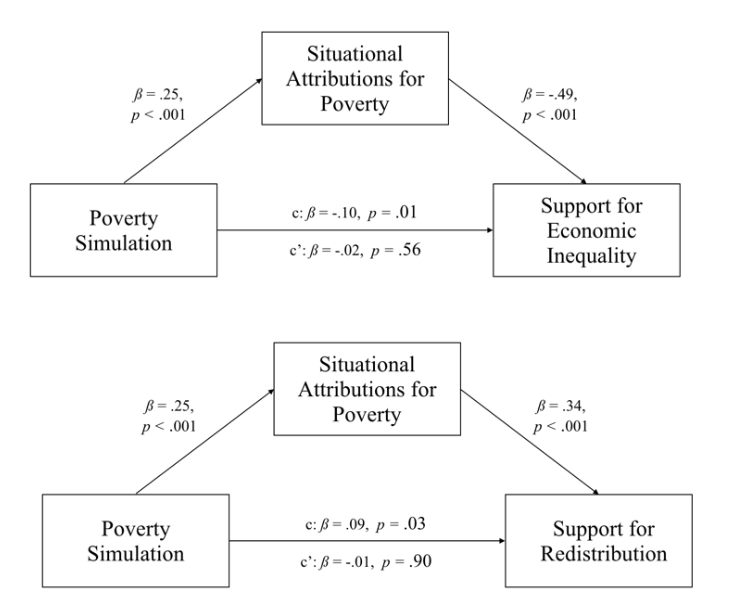
\includegraphics[width=\linewidth]{Fig3-1.png}
  \caption{Mediation models in Study 2b demonstrating that the online poverty simulation SPENT influences both Support for Economic Inequality and Support for Redistribution through increased situational attributions for poverty}
  \label{fig:thirdfig}
\end{figure}

\subsubsection{Exploratory Analyses}

To explore the longevity of the SPENT poverty simulation intervention on support for economic inequality, I conducted two follow-up surveys. First, participants completed a follow-up survey (identical to the initial survey) the day following their original, in-lab participation (Time 2). Secondly, I conducted one additional follow-up upon completion of the data collection (Time 3) in mid-May 2018. In the Time 3 survey I invited participants to complete one additional follow-up survey in exchange for a chance to win one of five \$500 cash prizes. Of the original 611 participants, 111 responded to this e-mail solicitation. Among these participants, the average time between the first and last surveys was five months (154.95 days), with the most recent, and most distant, participants having 44 and 246 days, respectively, between their first and last survey completion.

\subparagraph{One Day Later} I tested whether the effects of playing SPENT (versus a no-game control condition) persisted one day after the manipulation by utilizing a series of two-tailed independent samples t-tests. Consistent with the immediate Time 1 analyses, participants reported higher situational attributions for poverty (\textit{t}(560) = 3.74, \textit{p} < .001, 95\% CI [.09, .29],  \textit{d} = .31), less support for economic inequality (\textit{t}(560) = -2.61, \textit{p} = .009, 95\% CI [-.36, -.05], \textit{d} = .22), and more support for redistribution (\textit{t}(560) = 2.19, \textit{p} = .03, 95\% CI [.01, .19], \textit{d} = .18) after the one day delay. Additionally, participants still did not exhibit a change in dispositional attributions for poverty (\textit{t}(560) = -1.40, \textit{p} = .16, 95\% CI [-.18, .03], \textit{d} = .05). Lastly, I tested whether situational attributions for poverty still mediated the relationship between playing SPENT and both support for economic inequality and redistribution using a simple mediation model with 1000 bootstrapped resamples. Higher situational attributions for poverty still mediated the effect of the poverty simulation on support for economic inequality (Indirect effect = -.16, \textit{p} < .001) and redistribution (Indirect effect = .20, \textit{p} = .02; Figure \ref{fig:fourthfig}).

\begin{figure}[h]
  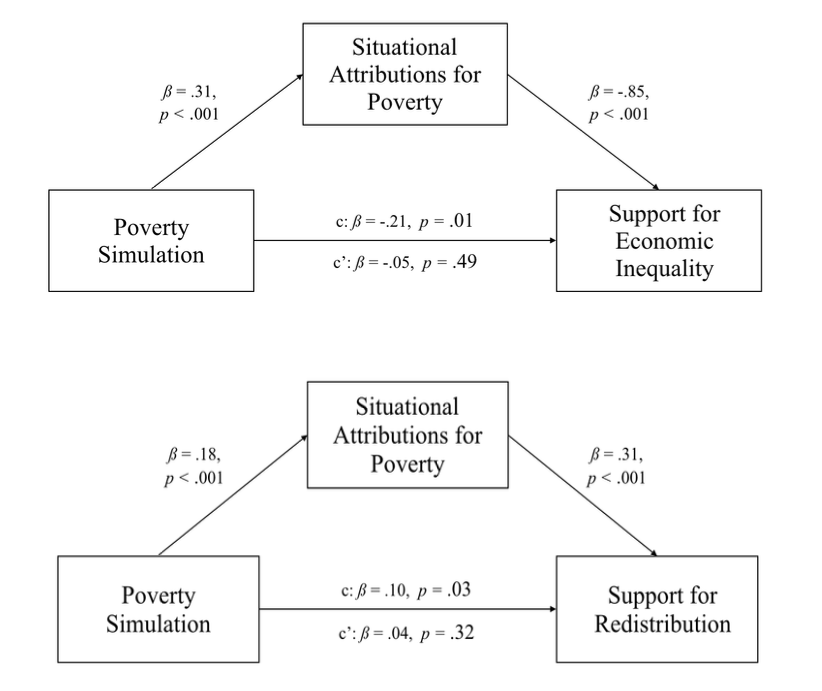
\includegraphics[width=\linewidth]{Fig3-2.png}
  \caption{Mediation models in Study 2b demonstrating that the online poverty simulation SPENT influences both support for economic inequality and support for redistribution through increased situational attributions for poverty at a one day delay}
  \label{fig:fourthfig}
\end{figure}

\subparagraph{Long-term Follow Up} At the Time 3 follow-up, an average five months following the initial manipulation, I found that the effects of the poverty simulation persisted. Consistent with the Time 1 and 2 analyses, participants who played SPENT (versus a no game control) reported higher situational attributions for poverty (\textit{t}(107) = 2.23, \textit{p} = .03, 95\% CI [.03, .53], \textit{d} = .45) and support for economic inequality (\textit{t}(107) = -2.54, \textit{p} = .01, 95\% CI [-.77, -.10], \textit{d} = .48). The effect of the poverty simulation did not persist on support for redistribution (\textit{t}(107) = .91, \textit{p} = .36, 95\% CI [-.11, .29], \textit{d} = .20), possibly due to insufficient power to detect the effect we observed with the relatively small sample size on this final follow-up. Additionally, consistent with the Time 1 and 2 analyses, situational attributions for poverty still mediated the relationship between the poverty simulation and support for economic inequality (Indirect Effect = .20, \textit{p} = .02), but not support for redistribution (Indirect Effect = -.06, \textit{p} = .08) an average of five months later.

Importantly, the effect of playing SPENT appears to hold on support for economic inequality regardless of the time between the manipulation and follow-up surveys. In order to statistically test this question, I ran two one-way ANOVAs wherein condition was entered as the main predictor of both support for economic inequality and redistribution and the number of days between surveys was entered as a continuous control variable. I found that playing SPENT had a significant impact on support for economic inequality, \textit{F}(1, 105) = 6.43, \textit{p} = .01 (Figure \ref{fig:fifthfig}), but not on support for redistribution when controlling for time between surveys, \textit{F}(1, 105) = .845, \textit{p} = .36 (Figure \ref{fig:sixthfig}). While limited by sample size, this pattern of results is promising because it suggests that a minor poverty simulation may have some long-term effects and is worth further exploration.

\begin{figure}
  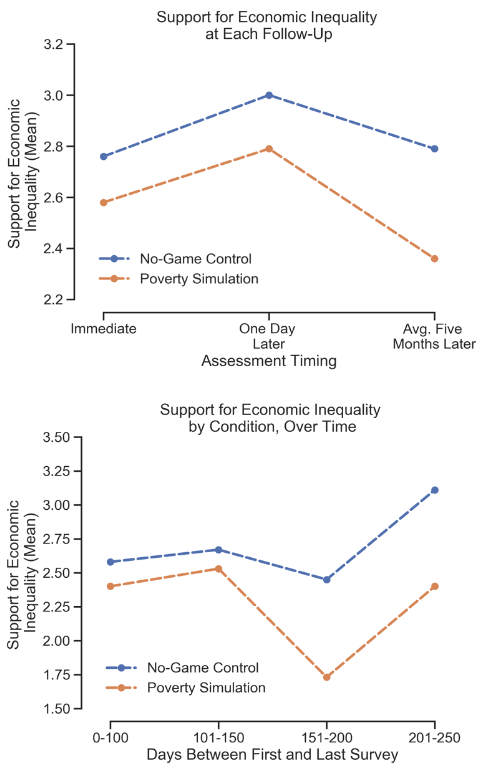
\includegraphics[scale=.75]{Fig3-3.png}
  \caption{Plots of support for economic inequality by both the time of assessment and average time between the Time 1 and Time 3 surveys}
  \label{fig:fifthfig}
\end{figure}

\begin{figure}
  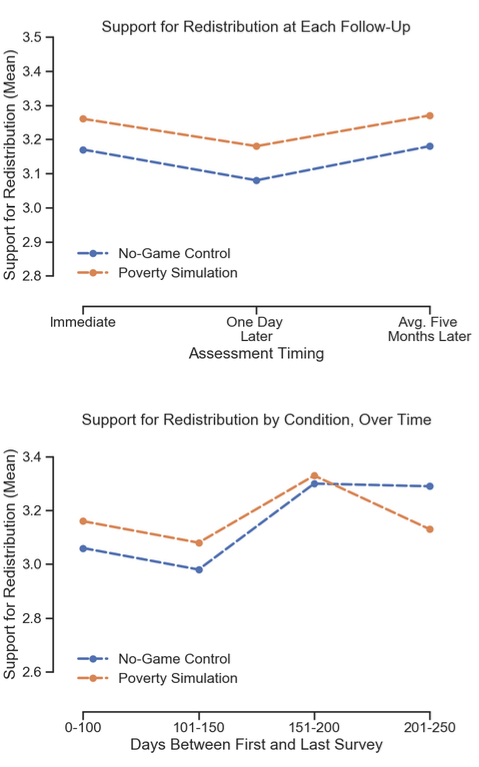
\includegraphics[scale=.75]{Fig3-4.png}
  \caption{Plots of support for economic inequality by both the time of assessment and average time between the Time 1 and Time 3 surveys}
  \label{fig:sixthfig}
\end{figure}

\subparagraph{Time 3 Hypothesis Recollection.} I had initially intended for the Time 2 survey (one day post-manipulation) to be the final survey and thus participants were debriefed at this point. In order to mitigate the possible demand characteristics resulting from the Time 3 participants knowing the hypothesis, I asked a series of questions designed to elicit the hypothesis. First, participants were told they “had participated in a study … in either the Fall 2017 or Winter 2018 term” in which they “came in to the lab … may or may not have played a short computer game, and then filled out a survey” before being asked if they recall participating. Unsurprisingly, most participants recalled having taken part in the study (n = 101; 91.8\%).

Second, I asked participants to “describe, in [their] own words, what this study was about” (full text responses at \href{https://osf.io/dkhs2/}{https://osf.io/dkhs2/}). While many participants recalled the survey was related to economic inequality, there were only four participants who recalled actual elements of the hypothesis, though none of which actually correctly stated the full hypothesis.\footnote{The four participants close to guessing the hypothesis wrote: “Based on … the survey, I'd say the study was about how people perceive those with low income and if the game changed that perspective,” “Experiencing the difficult choices made by people experiencing poverty and the influence of these experiences on attitudes and beliefs about poverty,” “Seeing how being in the shoes of someone poor, as someone who’s not poor, affects empathy for their issues and how they come to be (them vs things happening to them),” and “… The short game that some of the participants played was meant to show them what it would be like living as someone in poverty and seeing if it would change the participants' perspective on the poor and if they would have more empathy for them after seeing what it would be like to live that way”).}

Third, I informed participants that “there were two conditions to this study and each participant [themselves] only completed one of them while in the lab.” Afterward, I asked if they “recalled what those two conditions were.” The vast majority of the participants could not recall the two conditions (n = 96; 87.2\%).

Fourth, I asked participants “what were the two conditions” and if they could only recall one to note that as well. Responding to this prompt, six participants were able to free recall the two conditions (i.e., playing SPENT versus not; full text at \href{https://osf.io/dkhs2/}{https://osf.io/dkhs2/}). The remaining 106 simply wrote “NA” as instructed if they could not recall.

Fifth, I asked participants whether or not they could “recall the specific hypothesis of the study [they] participated in (i.e., what question the researchers were testing.” Again, the vast majority (n = 105; 94.6\%) reported they could not recall the hypothesis. I then asked participants specifically “what was the hypothesis;” no participants were actually able to articulate the hypothesis. Three participants were close in reporting they believed the hypothesis was that SPENT (versus the no-game control) would increase empathy for the poor.

Lastly, I presented participants with a multiple-choice question containing the true hypothesis (i.e., “playing a computer game (versus not) would decrease tolerance for economic inequality) and five distractors (i.e., playing a computer game (versus not) would (a) positively affect your mood, (b) increase tolerance for economic inequality, (c) improve your memory, (d) negatively affect your mood, (e) decrease your memory). On this question, thirty-three participants (30\% of the sample) correctly identified our hypothesis.

To ensure that the Time 3 effect was not being driven entirely by those participants who were able to identify our hypothesis in the final multiple-choice question, I re-ran the key analyses as a set of one-way ANOVAs controlling for whether or not participants got this question right. I found that being able to correctly guess the hypothesis did not predict either situational attributions for poverty (\textit{F}(1,106) = 1.34, \textit{p} =.25) or support for economic inequality (\textit{F}(1,105) = .01, \textit{p} =.93). More importantly, the effects of playing SPENT remained significant on both situational attributions for poverty (\textit{F}(1,106) = 4.99, \textit{p} =.03) and support for economic inequality (\textit{F}(1,105) = 6.40, \textit{p} =.01) when I entered correct hypothesis guess as a covariate.

For situational attributions for poverty, the observed effect was weaker for participants who incorrectly identified the hypothesis (correct: \textit{d} = .54; incorrect: \textit{d} = .33). This suggests that the participants who correctly identified the hypothesis may be artificially inflating the observed effect at time three, and the true effect is closer to a Cohen’s d of .32 rather than the observed Cohen’s d of .49 in the complete sample. Additionally, for support for economic inequality, the effect was again weaker for participants who incorrectly identified the hypothesis (correct: \textit{d} = .93; incorrect: \textit{d} = .32). It is possible that those who correctly identified the hypothesis artificially inflated the observed effect at Time 3, and the true effect is closer to a Cohen’s d of .32 rather than the observed Cohen’s d of .49 in the complete sample. However, given the extremely small sample sizes (33 correct, 78 incorrect) I suggest interpreting these effects with caution as they are likely to be rather unreliable effect size estimates.

\subparagraph{Causal Attributions for Other Behaviours} In order to explore whether playing SPENT impacts underlying causal attributions more broadly or specifically attributions for poverty, I measured causal attributions towards six other targets/concepts: obese people, criminals, general financial situation, wealth, inequality, and general behaviour. I tested whether or not engaging in the intensive poverty simulation of SPENT impacted these broader causal attributions by utilizing a series of two-tailed independent samples t-tests to compare average responses across conditions. On nearly every measure of broad causal attributions I found that there was no difference across conditions (Table \ref{tab:fifthtable}).

There were, however, two exceptions: playing SPENT (a) increased economic attributions for crime and (b) decreased dispositional attributions for wealth (Table 3.3). In hindsight, these findings are rather unsurprising as it is possible that learning about the situational causes of poverty and being exposed to the hardships of trying to make ends meet on such limited resources, could lead people to be more understanding of how economic factors might drive people to turn to crime, and how it is extremely difficult to create wealth when starting at the bottom. While these are admittedly post-how interpretations, I do not find these results entirely surprising. Additionally, these findings remain consistent with my suggestion that engaging in the poverty simulation is predominantly influencing attributions towards poverty. In order to ensure that these changed attributions for crime and wealth were not driving the effects of playing SPENT on support for economic inequality or redistribution, I re-ran these analyses as one-way ANOVAS controlling for economic attributions for crime and dispositional attributions for wealth. The effects of SPENT remained consistent on both support for economic inequality, \textit{F}(1, 604) = 6.63, \textit{p} = .01, and support for redistribution, \textit{F}(1, 604) = 5.40, \textit{p} = .02.

\begin{table}[h]
  \begin{center}
    \caption{Broad causal attributions by condition in Study 2b}
    \label{tab:fifthtable}
    \begin{tabular}{l c c c c}
    \hline
      & \multicolumn{1}{c}{SPENT} & \multicolumn{1}{c}{Monopoly} & & \\
      & \multicolumn{1}{c}{Game} & \multicolumn{1}{c}{Control} & & \\\cmidrule{2-3}
      & \multicolumn{1}{c}{M (SD)} & \multicolumn{1}{c}{(M (SD)} & t-test & Cohen's d\\
      \hline
      Obesity - Genetics & \multicolumn{1}{c}{4.32 (1.00)} & \multicolumn{1}{c}{4.43 (.97)} & \multicolumn{1}{c}{\textit{t}(607) = -1.28, \textit{p} = .20} & .10\\
      Obesity - Dispositional & \multicolumn{1}{c}{4.04 (.85)} & \multicolumn{1}{c}{4.09 (.83)} & \multicolumn{1}{c}{\textit{t}(607) = -.67, \textit{p} = .50} & .06\\
      Obesity - Situational & \multicolumn{1}{c}{4.33 (.98)} & \multicolumn{1}{c}{4.37 (1.00)} & \multicolumn{1}{c}{\textit{t}(607) = -.58, \textit{p} = .56} & .05\\
      Crime - Economic & \multicolumn{1}{c}{3.91 (.85)} & \multicolumn{1}{c}{3.72 (.76)} & \multicolumn{1}{c}{\textit{t}(605) = -1.05, \textit{p} = .004} & .23\\
      Crime - Dispositional & \multicolumn{1}{c}{3.92 (.95)} & \multicolumn{1}{c}{3.99 (.90)} & \multicolumn{1}{c}{\textit{t}(605) = -1.28, \textit{p} = .20} & .09\\
      Crime - Situational & \multicolumn{1}{c}{4.99 (.82)} & \multicolumn{1}{c}{5.06 (.83)} & \multicolumn{1}{c}{\textit{t}(605) = -1.09, \textit{p} = .28} & .09\\
      Financial Situation - Luck & \multicolumn{1}{c}{3.39 (1.24)} & \multicolumn{1}{c}{3.40 (1.30)} & \multicolumn{1}{c}{\textit{t}(606) = -.21, \textit{p} = .83} & .02\\
      Financial Situation - Family & \multicolumn{1}{c}{5.06 (1.08)} & \multicolumn{1}{c}{4.99 (.96)} & \multicolumn{1}{c}{\textit{t}(606) = .77, \textit{p} = .44} & .06\\
      Financial Situation - Dispositional & \multicolumn{1}{c}{5.42 (.78)} & \multicolumn{1}{c}{5.49 (.68)} & \multicolumn{1}{c}{\textit{t}(606) = -1.10, \textit{p} = .27} & .09\\
      Financial Situation - Situational & \multicolumn{1}{c}{4.79 (.76)} & \multicolumn{1}{c}{4.79 (.72)} & \multicolumn{1}{c}{\textit{t}(606) = .05, \textit{p} = .96} & .00\\
      Wealth - Dispositional & \multicolumn{1}{c}{3.12 (.77)} & \multicolumn{1}{c}{3.25 (.75)} & \multicolumn{1}{c}{\textit{t}(607) = -2.12, \textit{p} = .03} & .17\\
      Wealth - Situational & \multicolumn{1}{c}{3.75 (.75)} & \multicolumn{1}{c}{3.72 (.72)} & \multicolumn{1}{c}{\textit{t}(607) = .60, \textit{p} = .55} & .05\\
      Inequality - Dispositional & \multicolumn{1}{c}{3.99 (.74)} & \multicolumn{1}{c}{4.05 (.70)} & \multicolumn{1}{c}{\textit{t}(599) = -.95, \textit{p} = .34} & .08\\
      Inequality - Situational & \multicolumn{1}{c}{3.81 (.58)} & \multicolumn{1}{c}{3.76 (.52)} & \multicolumn{1}{c}{\textit{t}(599) = 1.21, \textit{p} = .23} & .10\\
      Causal Attributions & \multicolumn{1}{c}{4.30 (.66)} & \multicolumn{1}{c}{4.34 (.63)} & \multicolumn{1}{c}{\textit{t}(605) = -.72, \textit{p} = .47} & .06\\
      \hline
    \end{tabular}
  \end{center}
\end{table}

\section{General Discussion}

Across two studies I found evidence that engaging in a short, but immerse, ten-minute online poverty simulation can alter attributions for poverty and, as a result, support for economic inequality. Specifically, playing SPENT, the online poverty simulation, versus Monopoly or a no-game control condition led to increased recognition of the situational causes of poverty which, in turn, led to decreased support for economic inequality and increased support for wealth redistribution.

Additionally, I found that the poverty simulation did not influence the vast majority of other, more broad, behavioral attributions thus appears to be specific to attributions for poverty. The specificity of this effect is helpful in ruling out alternative explanations for the finding that situational attributions of poverty play a directly causal role in diminished support for economic inequality. For example, if we did not have information regarding the specificity of the poverty simulation on causal attributions it could be plausible that engaging in playing SPENT is causing other psychological shifts. For example, one of the most plausible alternative explanations is that the poverty simulation simply increases feelings of empathy or kindness towards any target (including the poor). Additional data from Study 2a help to rule out elevated levels of empathy as an alternative explanation because I did not observe differences in empathy after playing SPENT (versus Monopoly).

Findings from Studies 2a and 2b indicate that the poverty simulation appears to influence support for inequality and redistribution preferences only through situational attributions for poverty. Though I initially predicted that SPENT would influence both dispositional and situational attributions, this prediction was not supported. As such, findings align with past research indicating that dispositional and situational attributions for poverty are not two ends of a spectrum, but rather unique and orthogonal~\cite{miller81, solomon78}. Therefore, increasing recognition of the situational causes of poverty does not necessitate a reduction in their dispositional attributions for poverty.

Though I did not predict this, in hindsight it is logical that the poverty simulation is primarily influencing situational attributions for poverty. While there is some peripheral information regarding the work habits of the player in SPENT (having a full-time job, etc) the focus is very much on external happenings. That is, almost every daily event (in the game) is focused on some unforeseen and uncontrollable circumstance befalling the player (e.g., a child getting sick, unexpected moving expenses). The results of Studies 2a and 2b suggest that situational attributions for poverty are one potent psychological lever for addressing complacency towards economic inequality. But can dispositional attributions for poverty be altered to affect similar change? In the following chapter, I turn my focus to this question.

\chapter{Cross-Socioeconomic Contact as a Means to Change Attributions for Poverty}

Chapter 3 demonstrated that (a) an underappreciation for the situational causes of poverty is a contributing factor in support for economic inequality, and (b) engaging in a short, but immersive, poverty simulation highlighting the situational causes of poverty can reduce support for economic inequality. However, the poverty simulation did not result in any reliable changes in dispositional attributions for poverty. Therefore, I have only demonstrated thus far that changing situational attributions for poverty is one potential method of reducing support for economic inequality. Is shifting dispositional attributions for poverty another potentially fruitful avenue for reducing support for economic inequality from its baseline?

Given that lay beliefs about poverty in the United States tend to focus on the worthiness and dispositional characteristics of both the poor and wealthy, I suspected that addressing dispositions directly would offer a significant route to decreasing support for economic inequality and increasing support for redistribution (e.g.,~\cite{cozzarelli01}). Given that situational and dispositional attributions appear to be orthogonal constructs~\cite{miller81, solomon78}, it is reasonable to assume that they would operate as two separate levers when it comes to forming downstream economic attitudes. That is, if changing situational attributions for poverty can lead to decreased support for economic inequality then changing dispositional attributions may allow us to do the same. One possible way to shift dispositional attributions for poverty is to address the stereotypes that are linked to these attributions.

Inherently tied to dispositional attributions for poverty is the stereotype that the poor are lazy or deserving of their economic station. This belief is embedded directly in the items used to measure dispositional attributions for poverty. For instance, according to the Stereotype Content Model~\cite{fiske02}, people view those who are poor or on welfare in the most uncharitable manner—low on both warmth and competence. Cozzarelli et al.,~\cite{cozzarelli01} showed in a sample of college students that (among other things) people view the poor as substantially less hardworking and lazier than the middle class. Therefore, one possible avenue to changing dispositional attributions for poverty is by combatting the stereotype that the poor are lazy and do not work hard. 

How can one address the stereotype that the poor are lazy? One possibility is to present “stereotype disconfirming evidence” or information that directly challenges the notion that the poor do not work hard. Past research indicates that there are two theoretical models regarding how presenting stereotype disconfirming evidence can change belief systems: the bookkeeping model and the conversion model. The bookkeeping model~\cite{rothbart81} suggests that belief change is a gradual process that results from exposure to numerous small instances of stereotype disconfirmation. In contrast, the conversion model~\cite{rothbart81} suggests that beliefs can change following a single salient and impactful instance of stereotype disconfirmation. For example, in one study participants were given descriptions of three members of the same sorority~\cite{gurwitz77}. In one condition, one sorority girl was described as having engaged in three stereotype disconfirming behaviours, and in the other the condition three sorority girls were described as having each engaged in one stereotype disconfirming behaviour. The authors found that one single instance of strong stereotype disconfirmation by one sorority girl was more effective at changing attitudes towards sorority girls than three small instances of stereotype disconfirmation each committed by a different sorority girl. This finding provides some empirical evidence for the conversion model for changing belief systems. Therefore, in line with this model, I aimed to create one strong instance of poverty stereotype disconfirmation through a cross-socioeconomic status interaction in which a participant interacts with an ostensibly poor person who exhibits stereotype-disconfirming behaviour. I aimed to explore whether this strong instance of stereotype disconfirmation would lead to decreased dispositional attributions for poverty, and consequently less support for economic inequality.

\section{Study 3a: Stereotype Disconfirmation and Support for Economic Inequality}

Given that situational and dispositional attributions appear to function as distinct but complementary pathways~\cite{miller81, solomon78}, and that people tend to make broadly dispositional attributions for poverty (e.g.,~\cite{cozzarelli01}), I opted to explore this other, potentially fruitful, avenue to understanding support for economic inequality. Across two studies in Chapter 3 I found that increasing participant’s understanding that there are external factors that contribute to poverty led to decreased support for economic inequality. Thus, in Chapter 4, I tested whether dispositional attributions for poverty also play a role in determining support for economic inequality. Specifically, I predicted that after being exposed to an instance of strong poverty-related stereotype disconfirmation (i.e., a hardworking, persistent poor person), participants would display weaker dispositional attributions for poverty, stronger situational attributions for poverty, as well as demonstrate less support for economic inequality and more support for redistribution. Additionally, I predicted that dispositional and situational attributions would mediate the effects of the stereotype disconfirming evidence on both support for economic inequality and redistribution.

\subsection{Methods}
\subsubsection{Participants}

To initially explore this question, I recruited 151 participants (\textit{M\textsubscript{age}} = 19.64, 71.5\% female) in the Spring 2017 semester through Simon Fraser University’s psychology department research participation system. Participants signed up for a thirty-minute study in exchange for course credit. A post-hoc sensitivity power analysis shows that this sample size gives enough power ($\beta$ = .20, $\alpha$ = .05) to detect an effect as small as Cohen’s d = .31.

\subsubsection{Procedure}

Upon arrival to the lab, participants were led to a room containing a circular table and two chairs. Participants were then told that the study was being conducted in pairs, and that their partner should arrive shortly. Approximately one minute later, a confederate posing as the second participant arrived at the lab and was led to the same room. The research assistant then repeated these same instructions (i.e., study is done in pairs, partner is already here) to the confederate in order to make it appear as though the confederate was a second participant.

The research assistant instructed the participant and confederate to engage in a five-minute conversation, ostensibly so that the participants could meet and get to know their partner before completing a group task. Specifically, participants interacted with the confederate by answering a series of relatively innocuous questions, the final question being “What did you do on your last summer vacation?” These questions were modeled after the fast-friends procedure~\cite{aron97}, in which participants take turns answering a series of increasingly intimate questions.
	
\subparagraph{Manipulation.} Embedded within these questions was the key manipulation: a question designed to reveal the confederate’s low or average socio-economic status (SES). Specifically, after asking “What did you do on your last summer vacation” participants were randomly assigned to hear the confederate explain their summer job and the situation surrounding their work. When answering this question, the confederate kept elements of their job description the same, except for small variation in the need for the job. In the low SES condition the confederate said \textit{“my parents work full-time and still need help financially so as much as I wish I didn’t have to work the whole summer it was important that I helped them out.”} Meanwhile, in the average SES condition the confederate said \textit{“I don’t really have to work because my parents help me out a lot, but it was nice to get some work experience and to have some extra money on the side”} (adapted from~\cite{horbergunpub}). Importantly, in both the low and average SES conditions, the confederate portrayed themselves as hardworking. Because there is a stereotype that the poor are often lazy and not hardworking (e.g.,~\cite{cozzarelli01}), the presentation of the confederate as hardworking in the low SES condition should serve as stereotype disconfirming evidence. In the low-SES condition the confederate is making it clear that they are financially struggling, despite the fact they are working full time to make ends meet not only for themselves, but for their parents as well. After the five-minute conversation, the research assistant escorted the participant and confederate to separate and private rooms to complete an online questionnaire.

\subsubsection{Measures}

Participants completed the same measures used in Study 2a.

\subparagraph{Attributions for Poverty.} Participants first reported their situational attributions for poverty on the twelve-item Guimond et al.,~\cite{guimond89} measure, containing both situational (\textit{M} = 3.46, \textit{SD} = .70, $\alpha$ = .79) and dispositional (\textit{M} = 2.50, \textit{SD} = .88, $\alpha$ = .84) subscales. Following this, participants completed the thirty-item Nickols and Nielsen~\cite{nickols11} measure of both situational (\textit{M} = 4.55, \textit{SD} = .66, $\alpha$ = .67) and dispositional (\textit{M} = 3.36, \textit{SD} = .63, $\alpha$ = .78) attributions for poverty.

\subparagraph{Support for Economic Inequality.} Participants completed the same five-item measure of support for economic inequality from Study 2a (\textit{M} = 2.57, \textit{S}D = .92, $\alpha$ = .82;~\cite{wiwadunpub}).

\subparagraph{Support for Redistribution.} Participants completed the same four-item measure of support for redistributions from Study 2a (\textit{M} = 3.22, \textit{SD} = .48, $\alpha$ = .70;~\cite{inglehart}).

\subparagraph{Empathy.} Participants reported their overall feelings of empathy on the twenty-one item Interpersonal Reactivity Index~\cite{davis80}. This scale contains three subscales: perspective taking \textit{(M} = 3.84, \textit{SD} = .58, $\alpha$ = .67), empathic concern (\textit{M} = 4.09, \textit{SD} = .60, $\alpha$ = .77), and personal distress (\textit{M} = 2.89, \textit{SD} = .66 $\alpha$ = .72).

\subparagraph{Demographics.} Lastly, participants reported the same series of demographics from Study 2a. Participants answered open ended questions reporting both their ethnicity and undergraduate major. Participants then reported their household (\textit{Median} = \$80,000 - \$90,000, \textit{SD} = 4.38), overall political ideology (\textit{M} = 3.06, \textit{SD} = 1.45), stance on social issues (\textit{M} = 2.99, \textit{SD} = 1.49), and stance on economic issues (\textit{M} = 3.32, \textit{SD} = 1.38). Lastly, participants reported their political party identification as Democrat, Independent, Republican, or other (Modal response Democrat).

\subsubsection{Participant Exclusions and Missing Data}

There were no participant exclusions in this study.\footnote{There was minimal missing data in the data set; 85\% of the columns contained no missing data, and of the columns that did contain missing values the highest missingness was 5.3\% (self-reported household income). Of the individual items that required compositing into scales, the highest missingness was two data points on an individual item. Thus, given the extremely small percentage of missing data, I did not test the assumption of MCAR and simply averaged over the missing items when compositing the scales.}

\subsection{Results}

All statistical analyses in this study were conducted using the R programming language and built in packages~\cite{rcore} and the R Studio user interface~\cite{rstudio16}. I utilized various additional packages to conduct the following analyses: I computed descriptive statistics using psych~\cite{revelle17}, effect sizes using effsize~\cite{torchiano17}, power analyses using pwr~\cite{champely18}, and path analyses using lavaan~\cite{rosseel12}. Given that this study was exploratory in nature, I analyzed the data in a relatively flexible manner. The results of these additional analyses were then pre-registered and tested in Study 3b. 

I hypothesized that participants exposed to a hard-working, low SES person (vs. hard working average SES person) through a lab-based interaction would report lower dispositional attributions for poverty and, in turn, lower support for economic inequality. I tested these hypotheses with a series of independent-samples t-tests and multiple mediation analyses.

As shown in Table \ref{tab:sixthtable}, analyses indicated that there were no statistically significant differences between the average and low SES conditions on all dependent variables. Mean differences, however, were generally in the predicted direction. Participants who interacted with the low SES confederate reported slightly higher situational and lower dispositional attributions for poverty, as well as more negative attitudes toward economic inequality (Table \ref{tab:sixthtable}). However, there was no effect of interacting with the hard-working poor confederate on support for economic inequality or redistribution. 

\begin{table}[h]
  \begin{center}
    \caption{Means, standard deviations, inferential statistics, and effect sizes for each of the dependent variables in Study 3a}
    \label{tab:sixthtable}
    \begin{tabular}{l c c c c}
    \hline
      & \multicolumn{1}{c}{Low-SES} & \multicolumn{1}{c}{Average-} & & \\
      & & \multicolumn{1}{c}{SES} & & \\\cmidrule{2-3}
      & \multicolumn{1}{c}{M (SD)} & \multicolumn{1}{c}{(M (SD)} & t-test & Cohen's d\\
      \hline
      Dispositional Attributions* & \multicolumn{1}{c}{2.44 (.86)} & \multicolumn{1}{c}{2.61 (.89)} & \multicolumn{1}{c}{\textit{t}(149) = -1.12, \textit{p} = .26} & .19\\
      Dispositional Attributions* & \multicolumn{1}{c}{3.52 (.68)} & \multicolumn{1}{c}{3.39 (.72)} & \multicolumn{1}{c}{\textit{t}(149) = 1.09, \textit{p} = .31} & .17\\
      Situational Attributions** & \multicolumn{1}{c}{3.33 (.68)} & \multicolumn{1}{c}{3.42 (.56)} & \multicolumn{1}{c}{\textit{t}(149) = -.82, \textit{p} = .41} & .14\\
      Situational Attributions** & \multicolumn{1}{c}{4.49 (.69)} & \multicolumn{1}{c}{4.59 (.64)} & \multicolumn{1}{c}{\textit{t}(149) = -.89, \textit{p} = .37} & .15\\
      Support for Economic Inequality & \multicolumn{1}{c}{2.50 (.98)} & \multicolumn{1}{c}{2.68 (.80)} & \multicolumn{1}{c}{\textit{t}(149) = -1.16, \textit{p} = .25} & .20\\
      Support for Redistribution & \multicolumn{1}{c}{3.21 (.48)} & \multicolumn{1}{c}{3.19 (.48)} & \multicolumn{1}{c}{\textit{t}(149) = .20, \textit{p} = .84} & .04\\
      \hline
    \end{tabular}
  \end{center}
  \textit{Note.} * denotes the Guimond et al.,~\cite{guimond89} measure of attributions for poverty and ** denotes the Nickols and Nielsen~\cite{nickols11} measure of attributions for poverty.
\end{table}

One possible reason for the null effects observed in this pilot is that a sizeable portion of participants were lower SES themselves. This is problematic for two reasons. First, it is possible that many participants did not endorse negative stereotypes about the poor if they are themselves low SES. Second, if participants were low SES then the interaction was, by definition, not a cross-SES interaction. Thus, if participants were effectively not engaging in stereotype disconfirming cross-SES contact, the manipulation is unlikely to have influenced perceptions of the poor. In the Study 3a sample, 17\% of participants reported having a household family income of less than \$40,000 per year—below Canada’s Low-Income Cut Off~\cite{statcan18}.

I conducted two analyses to test the possibility that low-SES participants were suppressing the predicted effects. First, I ran a series of regressions (using z-scores) predicting each of the main dependent variables with condition assignment, participant’s reported income, and an interaction term (z-score of condition x z-score of income) as predictors. If a significant portion of contact with the low-SES participant was inadvertently same-SES contact I would expect an interaction, such that the main effect of condition emerges with high-SES participants but not with low-SES participants. Counter to this expectation, I found that there were no significant interactions between income and condition assignment on attributions for poverty, support for economic inequality, and support for redistribution (all \textit{ps} > .33). This suggests that a large portion of the participants being low SES is not a problem in this study. However, the non-significant interactions may simply be a result of the low power in this study to detect such interactions.
	
Therefore, I conducted a second analysis to help determine whether a significant portion of inadvertent same-SES contact might be suppressing the potential impact of the cross-SES interaction. Specifically, I conducted a median split on income (low income coded as reported household income at or below \$79,999, high income coded as reported household income at or above \$80,000). Following the median split, I computed Cohen’s d effect sizes for the mean differences on attributions for poverty, support for economic inequality, and support for redistribution in each group. All mean differences are in the predicted direction for both high (n = 79) and low-income (n = 64) groups. Crucially, effect sizes on almost all dependent variables, in particular dispositional attributions for poverty, were substantially larger for high-income participants relative to low-income participants (Table \ref{tab:seventhtable}). Due to the small sample sizes, these additional analyses should be interpreted with caution; with that in mind, this exploration of effect sizes provides a small amount of suggestive evidence that the null main effects observed in Study 3a may stem, at least in part, from a high proportion of self-identified low-income participants in the study. 

\begin{table}[h]
  \begin{center}
    \caption{Cohen’s d effect sizes for mean difference between the low and average socioeconomic contact conditions, across high and low socioeconomic status participants}
    \label{tab:seventh}
    \begin{tabular}{l c c}
    \hline
      & \multicolumn{1}{c}{Low-SES} & \multicolumn{1}{c}{High-SES}\\\cmidrule{2-3}
      & \multicolumn{1}{c}{Cohen's d)} & \multicolumn{1}{c}{(Cohen's d)}\\
      \hline
      Dispositional Attributions* & \multicolumn{1}{c}{.01} & \multicolumn{1}{c}{.42}\\
      Dispositional Attributions* & \multicolumn{1}{c}{.02} & \multicolumn{1}{c}{.26}\\
      Situational Attributions** & \multicolumn{1}{c}{.17} & \multicolumn{1}{c}{.42}\\
      Situational Attributions** & \multicolumn{1}{c}{.21} & \multicolumn{1}{c}{.08}\\
      Support for Economic Inequality & \multicolumn{1}{c}{.12} & \multicolumn{1}{c}{.28}\\
      Support for Redistribution & \multicolumn{1}{c}{.05} & \multicolumn{1}{c}{.01}\\
      \hline
    \end{tabular}
  \end{center}
  \textit{Note.} * denotes the Guimond et al.,~\cite{guimond89} measure of attributions for poverty and ** denotes the Nickols and Nielsen~\cite{nickols11} measure of attributions for poverty.
\end{table}

\subsection{Discussion}

Counter to my predictions, stereotype disconfirmation through cross-SES contact with a low SES confederate did not change attributions for poverty, support for economic inequality, or support for redistribution. There are numerous possible reasons for these null effects. First and foremost, it is entirely possible that instances of stereotype disconfirmation do not impact attributions for poverty, and therefore the present manipulation was unsuccessful in influencing dispositional attributions for poverty and support for economic inequality.

However, it is also possible that Study 3a was too underpowered to properly test this question and further undermined by a high degree of inadvertent same-SES contact. There are three possible reasons this alternative explanation is plausible. First, the evidence that the confederate was hardworking (thus, stereotype disconfirming) was subtle and implied—the confederate merely mentioned their socioeconomic status once during a five-minute conversation and the critical information was embedded in a story about their summer vacation. Second, presentation of socioeconomic status occurred immediately before the participant completed the dependent measures, giving little time for the participant to process the information they had just heard. Because the confederate presented this information, and then immediately left the interaction to complete the questionnaire, it is possible the participant did not even take note of this information. Lastly, given that the manipulation was subtle, the effect sizes I observed were small—around Cohen’s d of .20. If this is the size of the effect I can observe with a subtle manipulation, the study was underpowered. Thus, I would require either (a) a larger sample to detect this effect, or (b) a stronger manipulation that is likely to elicit a larger effect. I opted to take both of these approaches in Study 3b. When exploring stereotype disconfirmation, I consider an effect size around Cohen’s d of .20 to be meaningful. If a single isolated instance of exposure to stereotype disconfirming evidence through cross-group contact can have an effect, even a small effect, there remains promise for the positive benefits of fostering this type of interaction. Additionally, I expect that if the stereotype disconfirmation were less subtle the effect would not be as small; therefore, these results are promising and justify conducted a follow-up study in which I address the aforementioned limitations.

A stronger manipulation of stereotype disconfirmation through cross-SES contact may be an effective tool for changing attributions for poverty and downstream attitudes. I thus aimed to test this possibility in Study 3b with a high powered pre-registered replication including a stronger and more salient instance of stereotype disconfirmation.

\section{Study 3b: Strengthening the Cross-Socioeconomic Status Contact, a High-Powered Pre-Registered Replication}

In Study 3a study I did not find any meaningful difference in attributions for poverty or support for economic inequality after participants engaged in a discussion with a low-SES (versus average-SES) confederate. Two potential reasons for this null finding are that the study was (a) underpowered and (b) the manipulation was too subtle. Thus, in Study 3b I conducted a high-powered, pre-registered follow-up study using a similar protocol with strengthened manipulation and increased sample size.

I also made several study design changes in line with those in Study 2b. Specifically, I measured causal attributions for other targets (i.e., obesity, crime, financial situation, wealth, inequality, and general behaviour). Including measures of more general causal attributions is crucial in understanding the mechanism of stereotype disconfirmation through cross-SES contact. Specifically, it allowed me to investigate whether I am simply addressing attributions for one specific group – people who live in poverty – or a person’s underlying attributional framework.

One final improvement in Study 3b was the inclusion of a behavioural dependent variable. In Studies 2a and 2b I did not uncover any relationship between attributions for poverty and support for redistribution. This is unsurprising, however, as supporting outright wealth redistribution as a means to addressing economic inequality is a complicated and partisan political issue. Thus, support for redistribution might be a hard attitude to move, especially with a small lab-based manipulation. Alternatively, a simple interaction with a low-SES confederate may cause change in a smaller, more action oriented dependent variable – giving directly to someone in poverty. Thus, in Study 3b I included a small raffle ticket dictator game to explore whether the cross-SES interaction leads to increased giving directly to the ostensibly low-SES confederate.

\subsection{Methods}
\subsubsection{Sample Size Determination}

I did not conduct an a priori power calculation to determine the sample size. Instead, I employed a two-step sequential analysis approach to the data collection due to the resource-intensive nature of the data collection (e.g., the study required coordinating the schedules of five research assistants, requiring three to be on hand for each thirty-minute data collection session). Sequential analysis was developed by Wald~\cite{wald47} as a method for more efficiently reaching conclusions when there are significant constraints on data collection. In the present study I used the O’Brien-Fleming boundary conditions with one interim analysis~\cite{obrien79}. Using this approach, I specified that I would analyze the data once following the conclusion of the Spring 2018 semester (April 15\textsuperscript{th}, 2018), with a one-tailed alpha set at .005 for the main hypotheses (1.1, 1.2, and 1.3). If this threshold was not met, data collection would continue until the end of the Fall 2018 semester (December 2018). I laid out the sequential analytic plan in the pre-registration document, which can be found on \href{https://osf.io/5cugx/register/5730e99a9ad5a102c5745a8a}{the OSF}.

As specified, I conducted the initial analyses in April 2018. However, I opted to stop data collection at this point despite the initial specified one-tailed alpha boundary (.005) being met for only one of these three main hypotheses. I made this decision not because I observed effects on the other two hypotheses that were traditionally (i.e., \textit{p} < .05) significant and “close enough,” but because the effects were so miniscule that further data collection would have been wasteful. For the two non-significant hypotheses, the observed effects were effectively 0 (Cohen’s ds of .02 and .003). After collection of nearly 250 participants I am confident that, for those two particular hypotheses, there is no true effect. Thus the data, and common sense, suggested stopping data collection; it is extremely unlikely any effects would emerge with further data collection. Additionally, it is important to note that sequential analysis is designed to protect a researcher from making Type I errors when analyzing their data early~\cite{malek17, wald47}. Therefore, the decision to stop data collection with null effects at this point does not subvert the intended protections of the sequential analysis.

\subsubsection{Participants}

I recruited 247 individuals (\textit{M\textsubscript{age}} = 21.8, 57\% Female) around campus at Simon Fraser University in exchange for \$5-10 CAD over the course of two semesters in Fall 2017 and Spring 2018.

\subsubsection{Procedure}

Study 3b was identical to Study 3a with just two changes to the procedure. First, in order to make the confederates’ low or average SES cues more salient, they wore one of two blue sweatshirts. In the low-SES condition the confederate wore a sweatshirt that was marginally worn with holes in the cuffs and pockets and the hood string missing in order to visually signal lower status. The average-SES participant, on the other hand, wore a brand-new version of the same sweatshirt (Figures \ref{fig:seventhfig} and \ref{fig:eighthfig}). 

\begin{figure}
  \begin{center}
    
\includegraphics[scale=.90]{Fig4-1a.png}
    \caption{Sweatshirt worn by the confederate in the low socioeconomic status condition}
    \label{fig:seventhfig}
  \end{center}
\end{figure}

\begin{figure}
  \begin{center}
    
\includegraphics[scale=.90]{Fig4-1b.png}
    \caption{Sweatshirt worn by the confederate in the high socioeconomic status condition}
    \label{fig:eighthfig}
  \end{center}
\end{figure}

Second, the confederate mentioned their SES, as well as their hardworking nature, twice during the participant-confederate interaction as opposed to the single mention of SES in Study 3a. Additionally, the confederate mentioned their SES and hardworking nature earlier in the interaction to allow for additional time for the participant to process this information before completing the final questionnaire. The first instance occurred in the response to the fifth of ten questions: “what is your major?” In both conditions the confederate stated that they have not declared their major in the Faculty of Arts and Social Sciences but are considering switching to computer science. However, the reason for this switch differed by condition.

In the low-SES condition the confederate said, \textit{“I grew up in a pretty poor household. Computer science and business seem like the best options for getting a job after I’m done my degree. Plus, I’m dependent on bursaries, and I think I can get bursaries if I switch to STEM. That will help me pay off my student loans.”}

In the average-SES condition, the confederate said, \textit{“Computer science and business seems like the best options for a challenging career. Plus, I think I can get bursaries if I switch to STEM. The extra spending money will be nice to have while I’m in school.” The second mention of both the SES and hardworking information was identical to Study 3a as the answer to the final question “What did you do on your last summer vacation?”}

\subsubsection{Measures}

Following the cross-SES interaction, participants completed the same set of measures as participants in Study 2b. All measures were completed in randomized order with demographics coming last.

\subparagraph{Attributions for Poverty.} Participants reported their attributions for poverty on the thirty-item Nickols and Nielsen~\cite{nickols11} measure consisting of both situational (\textit{M} = 4.57, \textit{SD} = .67, $\alpha$ = .65) and dispositional (\textit{M} = 3.13, \textit{SD} = .64, $\alpha$ = .76) attributions for poverty subscales.

\subparagraph{Support for Economic Inequality.} Participants reported their support for economic inequality on the same five-item scale from Study 3a (~\cite{wiwadunpub}; \textit{M} = 2.51, \textit{SD} = 1.11, $\alpha$ = .87).

\subparagraph{Attributions for Affluence.} Participants reported their attributions for affluence on the four-item~\cite{furnham83} scale. This scale was designed to measure both internal (\textit{M} = 3.15, \textit{SD} = .90, $\alpha$ = .63) and external (\textit{M} = 3.85, \textit{SD} = .78, $\alpha$ = .51) attributions for wealth.

\subparagraph{Attributions for Financial Situation.} Participants reported their attributions for financial situation on the fifteen-item scale adapted from Forgas, Morris, and Furnham~\cite{forgas82}. The complete scale contains four subscales: internal (\textit{M} = 5.29, \textit{SD} = 1.00, $\alpha$ = .75), external (\textit{M} = 4.78, \textit{SD} = .82, $\alpha$ = .48), family (\textit{M} = 5.09, \textit{SD} = 1.13, $\alpha$ = .59), and luck (\textit{M} = 3.37, \textit{SD} = 1.37, $\alpha$ = .53).

\subparagraph{Attributions for Obesity.} Participants reported their attributions for obesity on the fifteen-item Klaczynski, et al,~\cite{klaczynski04} scale. The complete scale intends to measure perceived causes of obesity and contains three subscales: internal (\textit{M} = 4.08, \textit{SD} = .92, $\alpha$ = .76), external (\textit{M} = 4.52, \textit{SD} =1.01, $\alpha$ = .69), and genetic (\textit{M} = 4.25, \textit{SD} = 1.17, $\alpha$ = .74).

\subparagraph{Attributions for Crime.} Participants reported their attributions for crime on a twelve-item scale~\cite{furnham83} ranging from 1 (Strongly Disagree) to 7 (Strongly Agree). The complete scale intends to measure perceived causes of crime and contains three subscales: internal (\textit{M} = 3.92, \textit{SD} = 1.07, $\alpha$ = .65), broad external (\textit{M} = 5.01, \textit{SD} = .89, $\alpha$ = .55), and economic (\textit{M} = 3.97, \textit{SD} = .91, $\alpha$ = .41).

\subparagraph{Causes of Inequality.} Participants reported what they believe to be the most important causes of the growing gap between the rich and the poor on the twelve-item Kraus, Piff, and Keltner~\cite{kraus09} scale. The complete scale contains two subscales: individual (\textit{M} = 3.85, \textit{SD} = .90, $\alpha$ = .89) and societal (\textit{M} = 3.85, \textit{SD} = .55, $\alpha$ = .66) causes of inequality.

\subparagraph{Broad Causal Attributions.} Participants responded to the same set of scenarios from Petersen, et al.,~\cite{petersen82} that were designed to measure how a person makes causal attributions for behaviour (\textit{M} = 4.31, \textit{SD} = .68, $\alpha$ = .23) scale. Consistent with Study 2b, this scale was extremely unreliable. As such, I conducted any analyses on the individual item level.

\subparagraph{Support for Redistribution.} Participants reported their support for redistribution on the same four-item World Values Survey~\cite{inglehart} scale as Study 3a (\textit{M} = 3.25, \textit{SD} = .60, $\alpha$ = .78).

\subparagraph{Meritocracy.} Participants reported the extent to which they believe society is meritocratic~\cite{zimmerman13}—that success is based on individual ability—on a 1 (Strongly Disagree) to 7 (Strongly Agree) scale. One sample item is “People who work hard do achieve success” (\textit{M} = 4.29, \textit{SD} = 1.34, $\alpha$ = .89).	

\subparagraph{Demographics.} Lastly, participants reported a series of demographics. Participants answered open-ended questions reporting both their ethnicity and undergraduate major. Participants reported their household income on the same scale as Study 2a (\textit{Median} = \$60,000 - \$70,000, \textit{SD} = 4.44). Participants reported their political ideology on the same three items ranging from Study 3a (overall ideology: \textit{M} = 3.06, \textit{SD} = 1.43; stance on social issues: \textit{M} = 2.92, \textit{SD} = 1.48; stance on economic issues: \textit{M} = 3.40, \textit{SD} = 1.58). Participants reported their political party identification on the same four-option question as Study 2a, except this time with Canadian political parties (Liberal, Conservative, New Democrat, other). The modal response was Liberal, with 42.5\% of the sample choosing this option.

\subparagraph{Dictator Game.} Following the completion of all the dependent measures, participants completed a short one-shot dictator game to provide a measure of generosity toward a person in poverty. The research assistant informed the participant that they must draw a slip of paper out of a cup for the next part of the study. Unbeknownst to them, both slips of paper contained the letter “D.” The research assistant then informed the participant that they have randomly been chosen to be the “decider” and will be given a small envelope to complete the next task. Inside the envelope were instructions for the game, ten raffle tickets, and two small envelopes labeled “For Me” and “For my Partner.” The written instructions informed the participants that each raffle ticket provided one entry into a draw for \$100 cash. Participants were then instructed that they could choose how many tickets they would like to give to their partner (i.e., the confederate) and how many they would like to keep for themselves. I chose a cash prize for the dictator game because if the participant wanted to help their ostensibly poor partner, one way to do so would be to give them more entries into the cash draw to possibly help ease their financial burden. This is a more direct instance of helping as opposed to giving them tickets to win, for example, an object such as a sweatshirt. Participants were told their choice of how many tickets they share is completely anonymous and this information will not be shared with their partner.

\subsubsection{Pre-Registered Hypotheses}

Building on Study 3a, I had five main hypotheses, and one secondary mediation hypothesis, for this follow-up study. The pre-registration document for this study can be found on the \href{https://osf.io/5cugx/register/5730e99a9ad5a102c5745a8a}{Open Science Framework}. Importantly, because my five main predictions were directional, as stated in the pre-registration document, I conducted one-tailed tests for each of the five main hypotheses. The five main hypotheses are as follows:

\begin{itemize}
  \item [1.1]	Participants who engage in an interaction with an ostensibly low SES confederate will display higher situational attributions for poverty than students who engage in an interaction with an ostensibly average SES confederate.\newline
  \item [1.2]	Participants who engage in an interaction with an ostensibly low SES confederate will display lower dispositional attributions for poverty than students who engage in an interaction with an ostensibly average SES confederate.\newline
  \item [1.3]	Participants who engage in an interaction with an ostensibly low SES confederate will display lower support for inequality than students who engage in an interaction with an ostensibly average SES confederate.\newline
  \item [1.4]	Participants who engage in an interaction with an ostensibly low SES confederate will give more raffle tickets to their partner in the dictator game than students who engage in an interaction with an ostensibly average SES confederate.\newline
  \item [1.5]	Participants who engage in an interaction with an ostensibly low SES confederate will display higher support for redistribution than students who engage in an interaction with an ostensibly average SES confederate.
\end{itemize}

\begin{flushleft}
The one secondary mediation hypothesis is as follows:
\end{flushleft}

\begin{itemize}
  \item [2.1]	Increased situational attributions for poverty and decreased dispositional attributions for poverty will mediate the relationship measured in hypotheses 1.3, 1.4, and 1.5.
\end{itemize}

\subsection{Results}

All statistical analyses in this study were conducted using the R programming language and built in packages~\cite{rcore} and the R Studio user interface~\cite{rstudio16}. I utilized various additional packages to conduct the following analyses: I computed descriptive statistics using psych~\cite{revelle17}, effect sizes using effsize~\cite{torchiano17}, power analyses using pwr~\cite{champely18}, and path analyses using lavaan~\cite{rosseel12}. See the \href{https://github.com/dwiwad/Dissertation/tree/master/Study3a_and_3b}{Github repository for this study} for all data pre-processing and reported analyses.

\subsubsection{Five Main Hypotheses}

I tested each of the five main predictions using a series of one-tailed independent samples t-tests. Counter to predictions, participants randomly assigned to interact with a low-SES (relative to average-SES) confederate did not report higher situational attributions for poverty (hypothesis 1.1). However, in line with my prediction, participants randomly assigned to interact with a low-SES (versus average-SES) confederate did display lower dispositional attributions for poverty (hypothesis 1.2; Table \ref{tab:eighthtable}). Participants who engaged with the low-SES (versus average-SES) confederate did not display less support for economic inequality (hypothesis 1.3), or more support for redistribution (hypothesis 1.5). Interestingly, participants did donate more raffle tickets to their partner when their partner was low, versus average, SES (hypothesis 1.4). Thus, two of the five main pre-registered hypotheses were confirmed.

\begin{table}[h]
  \begin{center}
    \caption{Means, standard deviations, inferential statistics, and effect sizes for each of the dependent variables in Study 3b}
    \label{tab:eighthtable}
    \begin{tabular}{l c c c c}
    \hline
      & \multicolumn{1}{c}{Low-SES} & \multicolumn{1}{c}{Avg-SES} & & \\
      & \multicolumn{1}{c}{Confederate} & \multicolumn{1}{c}{Confederate} & & \\\cmidrule{2-3}
      & \multicolumn{1}{c}{M (SD)} & \multicolumn{1}{c}{(M (SD)} & t-test & Cohen's d\\
      \hline
      Dispositional Attributions & \multicolumn{1}{c}{3.02 (.62)} & \multicolumn{1}{c}{3.24 (.64)} & \multicolumn{1}{c}{\textit{t}(245) = -2.72, \textit{p} = .003} & .35\\
      Situational Attributions & \multicolumn{1}{c}{4.56 (.67)} & \multicolumn{1}{c}{4.58 (.68)} & \multicolumn{1}{c}{\textit{t}(245) = -.18, \textit{p} = .57} & .02\\
      Support for Economic Inequality & \multicolumn{1}{c}{2.51 (1.10)} & \multicolumn{1}{c}{2.51 (1.13)} & \multicolumn{1}{c}{\textit{t}(245) = -.03, \textit{p} = .49} & .00\\
      Support for Redistribution & \multicolumn{1}{c}{3.29 (2.08)} & \multicolumn{1}{c}{3.22 (1.81)} & \multicolumn{1}{c}{\textit{t}(245) = .90, \textit{p} = .18} & .12\\
      Raffle Tickets Donated & \multicolumn{1}{c}{5.84 (.51)} & \multicolumn{1}{c}{5.06 (.52)} & \multicolumn{1}{c}{\textit{t}(245) = 3.15, \textit{p} < .001} & .40\\
      \hline
    \end{tabular}
  \end{center}
\end{table}

\subsubsection{Mediation Models}

To test the prediction that attributions for poverty mediate the relationships between the cross-SES interaction and (a) support for economic inequality, (b) number of raffle tickets donated, and (c) support for redistribution (hypothesis 2.1), I conducted three separate mediation analyses with both situational and dispositional attributions for poverty entered simultaneously as mediators between condition assignment and each dependent variable. In the first model, a multiple mediation model with 1,000 bootstrapped resamples showed that engaging with the low-SES confederate did not increase situational attributions for poverty but did decrease dispositional attributions for poverty (Figure \ref{fig:ninthfig}). Crucially, only diminished dispositional attributions for poverty mediated the relationship between cross-SES contact and support for economic inequality (Indirect effects = -.01, \textit{p} = .86 and .04, \textit{p} = .02, through situational and dispositional attributions respectively). This finding suggests that cross-SES contact with a low-SES confederate impacts support for economic inequality by reducing dispositional attributions for poverty. 

\begin{figure}
  \begin{center}
    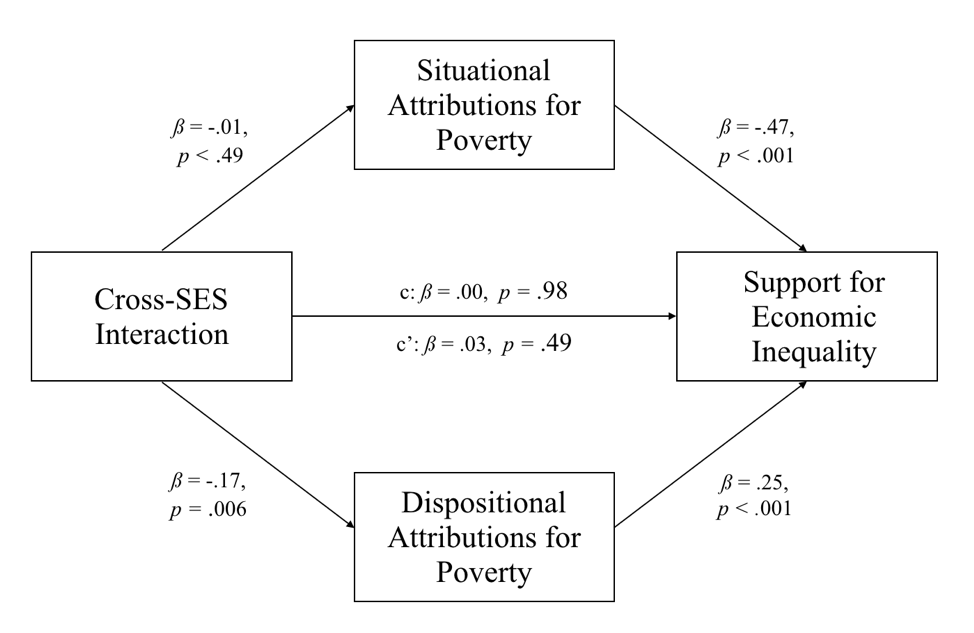
\includegraphics[scale=.75]{Fig4-3.png}
    \caption{Mediation model in Study 3b demonstrating that cross-SES contact influences support for economic inequality through decrease dispositional attributions for poverty}
    \label{fig:ninthfig}
  \end{center}
\end{figure}

In the second model, I ran a multiple mediation model with 1,000 bootstrapped resamples to test the prediction that attributions for poverty mediate the relationship between cross-SES contact and the number of raffle tickets given to the confederate. I found that engaging with the low-SES confederate did not increase situational attributions for poverty but did decrease dispositional attributions for poverty (Figure \ref{fig:tenthfig}). Crucially, only lower dispositional attributions for poverty predicted the number of tickets given (Indirect effects = .00, \textit{p} = .77 and .04, \textit{p} = .03, through situational and dispositional attributions respectively). 

\begin{figure}
  \begin{center}
    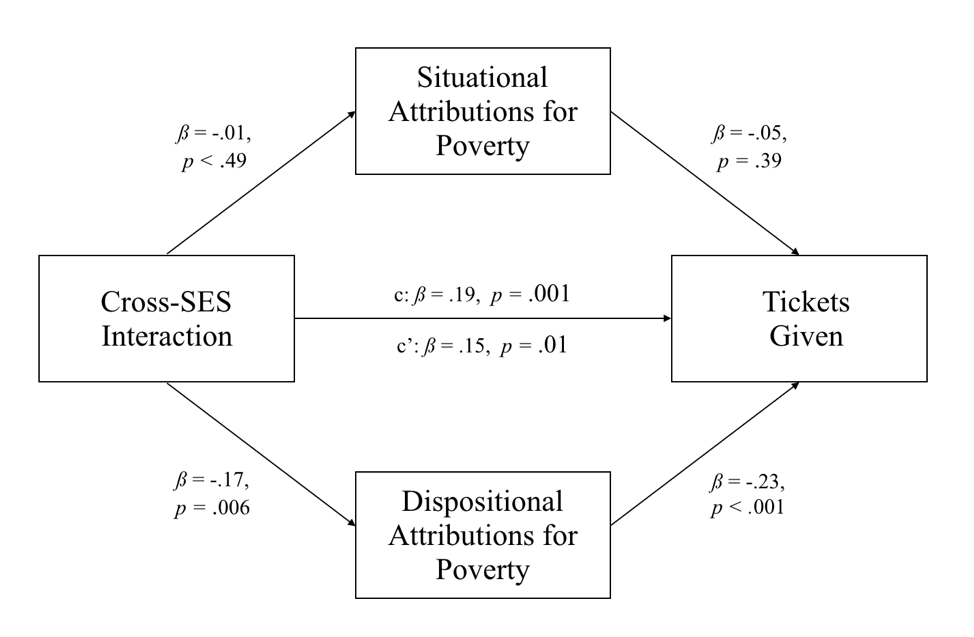
\includegraphics[scale=.75]{Fig4-4.png}
    \caption{Mediation model in Study 3b demonstrating that cross-SES contact influences the number of raffle tickets given to a confederate through decrease dispositional attributions for poverty}
    \label{fig:tenthfig}
  \end{center}
\end{figure}

In the final model, I ran a multiple mediation model with 1,000 bootstrapped resamples to test the prediction that attributions for poverty mediate the relationship between cross-SES contact and support for redistribution. I found that engaging with the low-SES confederate did not increase situational attributions for poverty but did increase dispositional attributions for poverty (Figure \ref{fig:eleventhfig}. In line with the previous two models, only lower dispositional attributions for poverty predicted increased support for redistribution (Indirect effects = .00, \textit{p} = .86 and .03, \textit{p} = .05, through situational and dispositional attributions respectively). 

\begin{figure}
  \begin{center}
    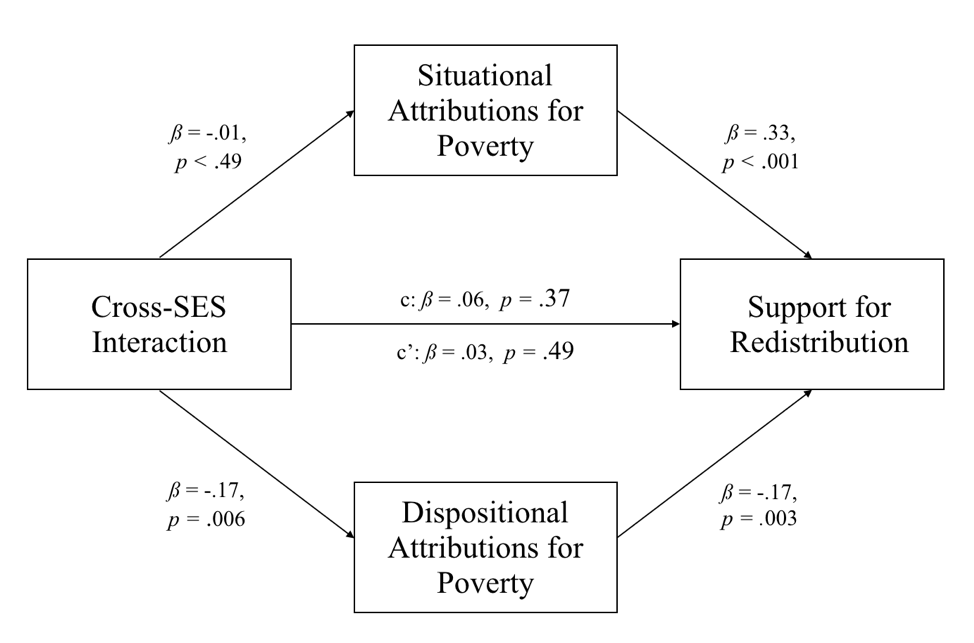
\includegraphics[scale=.75]{Fig4-5.png}
    \caption{Mediation model in Study 3b demonstrating that cross-SES contact influences the number of raffle tickets given to a confederate through decrease dispositional attributions for poverty}
    \label{fig:eleventhfig}
  \end{center}
\end{figure}

\subsubsection{Exploratory Analyses}

\subparagraph{Broad Causal Attributions.} In order to explore whether engaging in a cross-SES interaction impacts underlying causal attributions more broadly or specifically attributions for poverty, I measured causal attributions towards six other targets: obese people, criminals, general financial situation, wealth, inequality, broad behaviour. I tested whether the cross-SES interaction impacted broader causal attributions by utilizing a series of two-tailed independent samples t-tests. I found that there was no change in the majority of broader causal attributions (Table \ref{tab:ninthtable}). There was one significant difference: the cross-SES interaction decreased the belief that one’s family is a factor in determining one’s financial situation (Table \ref{tab:ninthtable}). \newpage

\begin{table}[h]
  \begin{center}
    \caption{Means, standard deviations, inferential statistics, and effect sizes for broad causal attributions in Study 3b}
    \label{tab:ninthtable}
    \begin{tabular}{l c c c c}
    \hline
      & \multicolumn{1}{c}{Low-SES} & \multicolumn{1}{c}{Avg-SES} & & \\
      & \multicolumn{1}{c}{Confederate} & \multicolumn{1}{c}{Confederate} & & \\\cmidrule{2-3}
      & \multicolumn{1}{c}{M (SD)} & \multicolumn{1}{c}{(M (SD)} & t-test & Cohen's d\\
      \hline
      Obesity - Genetics & \multicolumn{1}{c}{4.22 (1.17)} & \multicolumn{1}{c}{4.28 (1.17)} & \multicolumn{1}{c}{\textit{t}(245) = -.67, \textit{p} = .50} & .05\\
      Obesity - Dispositional & \multicolumn{1}{c}{4.04 (.92)} & \multicolumn{1}{c}{4.12 (.93)} & \multicolumn{1}{c}{\textit{t}(245) = -.40, \textit{p} = .69} & .09\\
      Obesity - Situational & \multicolumn{1}{c}{4.49 (1.06)} & \multicolumn{1}{c}{4.54 (.97)} & \multicolumn{1}{c}{\textit{t}(245) = -.39, \textit{p} = .70} & .05\\
      Crime - Economic & \multicolumn{1}{c}{3.96 (.83)} & \multicolumn{1}{c}{3.98 (.98)} & \multicolumn{1}{c}{\textit{t}(245) = -.15, \textit{p} = .88} & .02\\
      Crime - Dispositional & \multicolumn{1}{c}{3.94 (1.09)} & \multicolumn{1}{c}{3.91 (1.05)} & \multicolumn{1}{c}{\textit{t}(245) = .21, \textit{p} = .83} & .03\\
      Crime - Situational & \multicolumn{1}{c}{5.01 (.92)} & \multicolumn{1}{c}{5.01 (.85)} & \multicolumn{1}{c}{\textit{t}(245) = .02, \textit{p} = .98} & .00\\
      Financial Situation - Luck & \multicolumn{1}{c}{3.34 (1.42)} & \multicolumn{1}{c}{3.40 (1.32)} & \multicolumn{1}{c}{\textit{t}(245) = -.35, \textit{p} = .72} & .04\\
      Financial Situation - Family & \multicolumn{1}{c}{4.90 (1.20)} & \multicolumn{1}{c}{5.27 (1.03)} & \multicolumn{1}{c}{\textit{t}(245) = -2.51, \textit{p} = .01} & .33\\
      Financial Situation - Dispositional & \multicolumn{1}{c}{5.38 (.93)} & \multicolumn{1}{c}{5.21 (1.06)} & \multicolumn{1}{c}{\textit{t}(245) = 1.32, \textit{p} = .19} & .17\\
      Financial Situation - Situational & \multicolumn{1}{c}{4.75 (.78)} & \multicolumn{1}{c}{4.80 (.87)} & \multicolumn{1}{c}{\textit{t}(245) = -.47, \textit{p} = .64} & .06\\
      Wealth - Dispositional & \multicolumn{1}{c}{3.17 (.86)} & \multicolumn{1}{c}{3.13 (.93)} & \multicolumn{1}{c}{\textit{t}(245) = .33, \textit{p} = .74} & .04\\
      Wealth - Situational & \multicolumn{1}{c}{3.80 (.75)} & \multicolumn{1}{c}{3.90 (.81)} & \multicolumn{1}{c}{\textit{t}(245) = -1.07, \textit{p} = .28} & .13\\
      Inequality - Dispositional & \multicolumn{1}{c}{3.93 (.82)} & \multicolumn{1}{c}{3.77 (.96)} & \multicolumn{1}{c}{\textit{t}(245) = 1.48, \textit{p} = .14} & .19\\
      Inequality - Situational & \multicolumn{1}{c}{3.79 (.59)} & \multicolumn{1}{c}{3.90 (.56)} & \multicolumn{1}{c}{\textit{t}(245) = -1.56, \textit{p} = .13} & .19\\
      Causal Attributions & \multicolumn{1}{c}{4.32 (.64)} & \multicolumn{1}{c}{4.30 (.71)} & \multicolumn{1}{c}{\textit{t}(245) = .22, \textit{p} = .82} & .03\\
      \hline
    \end{tabular}
  \end{center}
\end{table}

\section{General Discussion}

Across two studies I found mixed evidence for the hypothesis that dispositional attributions for poverty offer another potent psychological lever for addressing complacency towards economic inequality and support for redistribution. Study 3a provided an initial test of this question but was likely too subtle and underpowered. Therefore, I conducted Study 3b – a well-powered, pre-registered replication. In Study 3b I found that engaging in a cross-SES interaction with a low status confederate (vs. average status confederate) led to participants make fewer dispositional attributions for poverty. However, I did not find any direct evidence that this interaction influenced support for economic inequality. Despite this lack of a direct effect, I did find that dispositional attributions for poverty mediated the relationship between condition assignment and support for economic inequality. Thus, there is some, albeit mixed, evidence that addressing dispositional attributions for poverty is another fruitful path to reducing complacency towards economic inequality.

Interestingly, despite this lack of movement on support for economic inequality, I found that participants who had a cross-SES interaction donated more raffle tickets (for a \$100 draw) to their partner. Why might there be an effect of addressing dispositional attributions for poverty on target-specific inequality-mitigating behavior but not on broad system-oriented support for economic inequality?

The poverty simulation I utilized in Studies 2a and 2b is primarily focused on abstract poverty; the player is encouraged to think about themselves as a person living in poverty. Outside of the player, there is no specific target. On the other hand, the manipulation I utilized in Studies 3a and 3b is focused directly on one specific target—the experimental confederate. Given the target-specificity of the manipulation, it is possible that changing dispositional attributions for poverty via a one-on-one interaction makes us want to help the specific target of that interaction while not necessarily changing broad system oriented lay-beliefs. It is also far easier to help one person in poverty than everyone who is poor. While I cannot address this rationale with the data in Study 3b, it is a promising avenue for future research in understanding the link between dispositional attributions for poverty and support for economic inequality. For example, future studies might attempt to shift situational attributions for poverty in a similar person-oriented fashion and shift dispositional attributions for poverty in a broad system-focused fashion and explore the downstream changes in support for economic inequality and willingness to help a specific target.

It is unclear whether attributions for poverty alone, or causal attributions more broadly can be utilized as a tool for reducing complacency towards economic inequality. In Chapters 3 and 4 I have utilized precise manipulations of attributions for poverty; these manipulations have not had any effect on broader causal attributions aimed at targets such as criminals, obese people, or towards financial situation and inequality more broadly. Thus, in Chapter 5 I focused on attempting to shift broad causal attributions and explore the downstream effects on support for economic inequality and redistribution.

\chapter{Causal Attributions for Other Behaviours}

In Chapters 3 and 4 of this dissertation I focused almost exclusively on efforts to shift poverty-specific causal attributions. Engaging in a poverty simulation increased situational attributions for poverty and engaging in the cross-SES interaction decreased dispositional attributions for poverty. However, neither of these manipulations influenced attributions of other targets (e.g., criminals, obese individuals). This suggests that the aforementioned manipulations were only influencing poverty specific attributions. However, the question remains: can repeatedly demonstrating the importance of context on human behavior alter attribution styles to impact support for economic inequality and redistribution? I tested this possibility in Study 4 using a quasi-experiment across seven undergraduate psychology classes.

\section{Study 4: Changing General Causal Attributions and Support for Economic Inequality}

In order to conduct a more direct test of whether it is underlying attributional style or attributions for poverty specifically that influence support for economic inequality and redistribution, I ran a quasi-experiment attempting to observe a shift in general causal attributions in a natural setting: the classroom. Particularly, in Introduction to Social Psychology at Simon Fraser University, the professor (Dr. Lara Aknin) focuses on “the power of the situation” as a course theme throughout the semester. Specifically, almost every lesson for the entire term reinforces the idea that the situation “has a large, and often underappreciated, effect on behavior.” Given the strong semester-long focus on understanding the situational causes of behavior, I sought to recruit participants across Introduction to Social Psychology (and several control classes) to explore whether shifting broad causal attributions for behaviour via semester long learning about the power of the situation would result in changes in poverty-specific attitudes—attributions for poverty, support for economic inequality, and support for redistributions.

\subsection{Methods}
\subsubsection{Participants}

Across two full semesters at Simon Fraser University (September-December 2017 and January-April 2018) I recruited an initial sample of 251 undergraduates (Mage = 20.8, 80.1\% Female) who were taking one (or more) of seven second year psychology classes: introduction to (a) abnormal (n = 11), (b) developmental (n = 81), (c) social (n = 106), (d) law (n = 6), (e) biological (n = 14), (f) cognitive (n = 12), and (g) data analysis in (n = 19) psychology. Participants taking Introduction to Social Psychology were considered the experimental group (n = 106), with all other students comprising the control group (n = 143). Given that the data collection for this study was completely dependent on the number of people from these classes who agreed to participate, I did not conduct any a priori power analyses. A total of 123 participants completed the Time 2 end of semester survey (attrition rate 51.0\%). This gave me only enough power (power = .80, $\alpha$ = .05) to detect an effect as small as Cohen’s d = .45. There appears to have been some degree of selective attrition across the conditions, with students in Introduction to Social Psychology (64.2\%) dropping out at a higher rate than participants across all six control classes (41.3\%; $\chi$\textsuperscript{2}(1) = 26.35, \textit{p} < .001). One possible reason for this uneven dropout may have been that I was the Teaching Assistant in the Introduction to Social Psychology classes. 

\subsubsection{Missing Data and Participant Exclusions}

Two participants did not enter their unique class identified codes. Therefore, I could not link these participants to either Introduction to Social Psychology, or a control class, and thus they were excluded from further analysis, leaving a final sample of 249. Additionally, the amount of missing data within the variables for compositing in this dataset was extremely minimal (0.48\%), and a test for the missing data on these 50 columns revealed that the missing data were MCAR ($\chi$\textsuperscript{2}(1) = 668.31, \textit{p} = .75. Thus, when compositing and analyzing the data I used listwise deletion because it is the least biased method.

\subsubsection{Procedure}

To recruit participants, I made an announcement in the first lecture of each of the seven introductory courses listed above in Fall 2017. The recruitment timing was critical, as in the second lecture of Introduction to Social Psychology the professor mentions “the power of the situation” as a guiding course theme. It is also important to note that the professor of this class deliberately did not draw any connections (e.g., in examples, demonstrations, etc) between the power of the situation and poverty, wealth, or inequality. In this announcement I invited all students in the class to take part in a two-part survey in exchange for an entry into a draw for a \$100 cash prize. Participants then either filled out the initial survey on paper immediately after the lecture or were given a link to a web survey they could complete later.

\subsubsection{Measures}

Almost all of the measures contained in this study are measures that I have used throughout this dissertation, with the excpetion of the manipulation check and demographics.

\subparagraph{Manipulation Check.} I used a modified version of the manipulation check from Shariff, Greene, Karremans, Luguri, Clark, Schooler, Baumeister, and Vohs~\cite{shariff14}. Specifically, in order to ensure that participants actually felt an increase in understanding of the causes of human behavior, they responded to the question “compared to the average Simon Fraser University student, how informed would you say you are about the causes of human behaviour?” on a 1 (Know much less than average) to 7 (Know a lot more than average) scale (\textit{M\textsubscript{Time 1}} = 4.64, \textit{SD} = 1.03; \textit{M\textsubscript{Time 2}} = 5.00, \textit{SD} = .94).

\subparagraph{Attributions for Poverty.} Participants reported their attributions for poverty on both the Guimond, et al.,~\cite{guimond89} and Nickols and Nielsen~\cite{nickols11} measures (Table \ref{tab:tenthtable}).

\begin{table}[h]
  \begin{center}
    \caption{Descriptive statistics for attributions for poverty in Study 4.}
    \label{tab:tenthtable}
    \begin{tabular}{l c c}
    \hline
      & \multicolumn{1}{c}{Time 1} & \multicolumn{1}{c}{Time 2}\\\cmidrule{2-3}
      & \multicolumn{1}{c}{M (SD)} & \multicolumn{1}{c}{(M (SD)}\\
      \hline
      Dispositional Attributions* & \multicolumn{1}{c}{2.23 (.89)} & \multicolumn{1}{c}{1.97 (.81)}\\
      Situational Attributions* & \multicolumn{1}{c}{3.51 (.75)} & \multicolumn{1}{c}{3.63 (.73)}\\
      Dispositional Attributions** & \multicolumn{1}{c}{3.78 (.34)} & \multicolumn{1}{c}{3.11 (.73)}\\
      Situational Attributions** & \multicolumn{1}{c}{3.87 (.41)} & \multicolumn{1}{c}{4.95 (.62)}\\
      \hline
    \end{tabular}
  \end{center}
  \textit{Note.} * denotes the Guimond et al.,~\cite{guimond89} measure of attributions for poverty and ** denotes the Nickols and Nielsen~\cite{nickols11} measure of attributions for poverty
\end{table}

\subparagraph{Support for Economic Inequality.} Participants reported their support for economic inequality on the five-item SEIS scale (\textit{M\textsubscript{Time 1}} = 2.66, \textit{SD} = .75; \textit{M\textsubscript{Time 2}} = 2.32, \textit{SD} = 1.00;~\cite{wiwadunpub}).

\subparagraph{Support for Redistribution.} Participants reported their support for redistribution on the four-item SEIS scale (\textit{M\textsubscript{Time 1}} = 3.80, \textit{SD} = .74; \textit{M\textsubscript{Time 2}} = 3.31, \textit{SD} = .55;~\cite{inglehart}).

\subparagraph{Demographics.} Lastly, participants reported a series of demographics. Participants answered open ended questions reporting their major (Modal response Psychology), year in university (\textit{Median} = 2, \textit{SD} = 1.06), every class they are taking in the term the completed the survey, and cumulative GPA (\textit{M} = 2.93, \textit{SD} = .70). Following this, participants checked off every introductory psych class they have taken in the past, from a list containing every second-year psychology course offered at SFU (introduction to: psychology I, psychology II, research methods, data analysis, cognitive, abnormal, developmental, social, law, and biological psychology). The question allowed me to account for any duplicate participant who was, for example, recruited in one of the control classes but is also taking Introduction to Social Psychology. Participants then reported their age, gender, and household income on the same scale used previously (\textit{Median} = \$70,000 - \$80,000, \textit{SD} = 4.24). Finally, participants reported their political ideology on the same three items used previously (overall ideology: \textit{M} = 2.92, \textit{SD} = 1.35; stance on social issues: \textit{M} = 2.50, \textit{SD} = 1.28; stance on economic issues: \textit{M} = 2.99, \textit{SD} = 1.38). Participants reported their political party identification on the same four option question used previously (Modal response Democrat, with 42.2\% of the sample choosing this option).

\subsubsection{Pre-Registered Hypotheses}

I pre-registered nine hypotheses (and analytic plan; osf.io/j2hmq/register/5730e99a9ad5a102c5745a8a). Note that I have truncated some of the language redundancies here for the sake of brevity.

\subparagraph{Attributions for Poverty.} First, I preregistered two hypotheses exploring whether, at the end of the semester, participants who took a semester-long course emphasizing the power of the situation would display different attributions for poverty than those who did not. Specifically, I predicted that:

\begin{itemize}
  \item [1.1]	Students who are currently taking introductory social psychology in the Fall 2017 and Winter 2018 terms at Simon Fraser University will display higher situational attributions for poverty at the end of the term (December 2017/April 2018) than students in the control classes.
  \item [1.2]	Students who are currently taking introductory social psychology in the Fall 2017 and Winter 2018 terms at Simon Fraser University will display lower dispositional attributions for poverty at the end of the term (December 2017/April 2018) than students in the control classes.
\end{itemize}

\begin{flushleft}
Second, I preregistered two hypotheses exploring whether there would be change over time in attributions for poverty for students who took the semester-long course emphasizing the power of the situation, and those who did not. I had two longitudinal hypotheses:
\end{flushleft}

\begin{itemize}
  \item [2.1]	Students who are currently taking introductory social psychology in the Fall 2017 and Winter 2018 terms at Simon Fraser University will display a greater increase in situational attributions for poverty between the beginning (September 2017/January 2018) and end (December 2017/April 2018) of the term than will students in the control classes.
  \item [2.2]	Students who are currently taking introductory social psychology in the Fall 2017 and Winter 2018 terms at Simon Fraser University will display a greater decrease in dispositional attributions for poverty between the beginning (September 2017/January 2018) and end (December 2017/April 2018) of the term than will students in the control classes.
\end{itemize}

\subparagraph{Support for Economic Inequality and Redistribution.} I preregistered two hypotheses exploring whether, at the end of the semester, participants who took a semester-long course emphasizing the power of the situation would display support for economic inequality and redistribution than those who did not. Specifically, I predicted that:

\begin{itemize}
  \item [3.1]	Students who are currently taking introductory social psychology in the Fall 2017 and Winter 2018 terms at Simon Fraser University will display higher support for redistribution at the end of the term (December 2017/April 2018) than students in the control classes.
\item [3.2]	Students who are currently taking introductory social psychology in the Fall 2017 and Winter 2018 terms at Simon Fraser University will display a greater increase in support for redistribution between the beginning (September 2017/January 2018) and end (December 2017/April 2018) of the term than will students in the control classes.
\end{itemize}

\begin{flushleft}
I also preregistered two hypotheses exploring whether there would be change over time in support for inequality and redistribution for students who took the semester-long course emphasizing the power of the situation, and those who did not. I had two longitudinal hypotheses:
\end{flushleft}

\begin{itemize}
  \item [3.3]	Students who are currently taking introductory social psychology in the Fall 2017 and Winter 2018 terms at Simon Fraser University will display lower support for economic inequality at the end of the term (December 2017/April 2018) than students in the control classes.
  \item [3.4]	Students who are currently taking introductory social psychology in the Fall 2017 and Winter 2018 terms at Simon Fraser University will display a greater decrease in support for economic inequality between the beginning (September 2017/January 2018) and end (December 2017/April 2018) of the term than will students in the control classes.
\end{itemize}

\begin{flushleft}
Lastly, I had one predicted interaction:
\end{flushleft}

\begin{itemize}
  \item [4.1]	I expect an interaction between class enrollment (introduction to social psychology versus control classes) and perceived knowledge of the causes of human behavior on support for economic inequality.
\end{itemize}

\subsection{Results}
\subsubsection{Baseline Tests}

Given that I did not randomly assign participants to condition, I needed to first verify that at Time 1 participants are roughly equivalent in attributions for poverty, support for economic inequality, and support for redistribution. In order to test this, I ran a series of two-tailed independent samples t-tests. Across both measures of attributions for poverty, as well as support for economic inequality and redistribution, there were no significant differences (Table \ref{tab:eleventhtable}). This demonstrates that, while there is no random assignment in this study, there was reasonable evidence that there were no baseline differences on the key measures. There was, however, a significant difference such that participants in the control classes reported more perceived knowledge of the causes of human behaviour than did participants in Introduction to Social Psychology at Time 1. 

\begin{table}[h]
  \begin{center}
    \caption{Means, standard deviations, inferential statistics, and effect sizes testing for baseline differences on key dependent variables in Study 4}
    \label{tab:eleventhtable}
    \begin{tabular}{l c c c c}
    \hline
      & \multicolumn{1}{c}{Intro Social} & \multicolumn{1}{c}{Control} & & \\
      & \multicolumn{1}{c}{Psychology} & \multicolumn{1}{c}{Classes} & & \\\cmidrule{2-3}
      & \multicolumn{1}{c}{M (SD)} & \multicolumn{1}{c}{(M (SD)} & t-test & Cohen's d\\
      \hline
      Percieved know. Human Behav. & \multicolumn{1}{c}{4.46 (.96)} & \multicolumn{1}{c}{4.77 (1.07)} & \multicolumn{1}{c}{\textit{t}(249) = 2.32, \textit{p} = .02} & .30\\
      Dispositional Attributions* & \multicolumn{1}{c}{2.30 (.90)} & \multicolumn{1}{c}{2.17 (.88)} & \multicolumn{1}{c}{\textit{t}(249) = -1.11, \textit{p} = .27} & .14\\
      Situational Attributions* & \multicolumn{1}{c}{3.51 (.70)} & \multicolumn{1}{c}{3.51 (.78)} & \multicolumn{1}{c}{\textit{t}(249) = -.03, \textit{p} = .97} & .00\\
      Dispositional Attributions** & \multicolumn{1}{c}{3.28 (.67)} & \multicolumn{1}{c}{3.20 (.73)} & \multicolumn{1}{c}{\textit{t}(248) = -.90, \textit{p} = .37} & .11\\
      Situational Attributions** & \multicolumn{1}{c}{4.69 (.68)} & \multicolumn{1}{c}{4.76 (.65)} & \multicolumn{1}{c}{\textit{t}(248) = .84, \textit{p} = .40} & .11\\
      Support for Economic Inequality & \multicolumn{1}{c}{2.45 (.93)} & \multicolumn{1}{c}{2.44 (.97)} & \multicolumn{1}{c}{\textit{t}(246) = -.09, \textit{p} = .92} & .01\\
      Support for Redistribution & \multicolumn{1}{c}{3.27 (.49)} & \multicolumn{1}{c}{3.30 (.51)} & \multicolumn{1}{c}{\textit{t}(249) = .50, \textit{p} = .62} & .06\\
      \hline
    \end{tabular}
  \end{center}
  \textit{Note.} * denotes the Guimond et al.,~\cite{guimond89} measure of attributions for poverty and ** denotes the Nickols and Nielsen~\cite{nickols11} measure of attributions for poverty
\end{table}

\subsubsection{Manipulation Check.}

To ensure that taking Introduction to Social Psychology had a greater effect on the perceived knowledge of the causes of behaviour than the control classes, I ran an independent samples t-test on the Time 2 data. Counter my predictions, I found no difference between the students taking Introduction to Social Psych (\textit{M} = 4.76, \textit{SD} = 1.08) and the students taking the control classes (\textit{M} = 5.11, \textit{SD} = 85; \textit{t}(120) = -1.90, \textit{p} = .06, 95\% CI [-.01, .70]). In fact, the means were in the opposite direction. Additionally, given the baseline differences in perceived knowledge, I utilized and independent samples t-test to explore whether students in Introduction to Social Psychology (\textit{M} = .14, \textit{SD} = .92) demonstrated a greater increase in perceived knowledge that students in the control classes (\textit{M} = .16, \textit{SD} = .84). However, I found no significant differences (\textit{t}(116) = .15, \textit{p} = .88, 95\% CI [-.31, .37]), suggesting that both groups had similar increases in perceived knowledge of the causes of human behavior over the course of the semester.

\subsubsection{Confirmatory Tests.}

First, I predicted that participants taking Introduction to Social Psychology would demonstrate higher situational (hypothesis 1.1), and lower dispositional (hypothesis 1.2) attributions for poverty than participants in the control classes at Time 2. To test these hypotheses, I ran a series of one-tailed independent samples t-tests. I found that students who learned explicitly about the power of the situation through taking a full semester of introduction to social psychology did not appear to report higher situational, or lower dispositional attributions at the end of the semester (Table \ref{tab:twelvthtable}). These finding suggests that either (a) there was no change in attributions for poverty over the semester, or (b) that participants in the experimental and control classes changed the same amount.

\begin{table}[h]
  \begin{center}
    \caption{Means, standard deviations, inferential statistics, and effect sizes testing for Time 2 differences on key dependent variables in Study 4}
    \label{tab:twelvthtable}
    \begin{tabular}{l c c c c}
    \hline
      & \multicolumn{1}{c}{Intro Social} & \multicolumn{1}{c}{Control} & & \\
      & \multicolumn{1}{c}{Psychology} & \multicolumn{1}{c}{Classes} & & \\\cmidrule{2-3}
      & \multicolumn{1}{c}{M (SD)} & \multicolumn{1}{c}{(M (SD)} & t-test & Cohen's d\\
      \hline
      Dispositional Attributions* & \multicolumn{1}{c}{2.13 (.84)} & \multicolumn{1}{c}{1.90 (.79)} & \multicolumn{1}{c}{\textit{t}(121) = -1.47, \textit{p} = .07} & .29\\
      Situational Attributions* & \multicolumn{1}{c}{3.47 (.69)} & \multicolumn{1}{c}{3.70 (.74)} & \multicolumn{1}{c}{\textit{t}(121) = 1.58, \textit{p} = .06} & .31\\
      Dispositional Attributions** & \multicolumn{1}{c}{3.17 (.64)} & \multicolumn{1}{c}{3.08 (.77)} & \multicolumn{1}{c}{\textit{t}(121) = -.60, \textit{p} = .27} & .12\\
      Situational Attributions** & \multicolumn{1}{c}{4.96 (.71)} & \multicolumn{1}{c}{4.95 (.58)} & \multicolumn{1}{c}{\textit{t}(121) = -.08, \textit{p} = .53} & .01\\
      Support for Economic Inequality & \multicolumn{1}{c}{2.41 (1.07)} & \multicolumn{1}{c}{2.29 (.97)} & \multicolumn{1}{c}{\textit{t}(120) = -.64, \textit{p} = .26} & .12\\
      Support for Redistribution & \multicolumn{1}{c}{3.24 (.53)} & \multicolumn{1}{c}{3.34 (.56)} & \multicolumn{1}{c}{\textit{t}(120) = .98, \textit{p} = .17} & .19\\
      \hline
    \end{tabular}
  \end{center}
  \textit{Note.} * denotes the Guimond et al.,~\cite{guimond89} measure of attributions for poverty and ** denotes the Nickols and Nielsen~\cite{nickols11} measure of attributions for poverty
\end{table}

Second, I predicted that students taking Introduction to Social Psychology would display a greater increase in situational (hypothesis 2.1), and greater decrease in dispositional (hypothesis 2.2), attributions for poverty between the beginning and end of the semester. I tested these predictions with a series of one-tailed independent samples t-tests on the difference scores between Times 1 and 2. Specifically, I subtracted Time 1 situational and dispositional attributions for poverty from the Time 2 measurements. In line with the previous findings, students who took introduction to social psychology did not experience any significantly stronger growth in situational attributions for poverty, or decline in dispositional attributions, than did the students in the control classes (Table \ref{tab:thirteenthtable}). Analyses testing the first four hypotheses suggest that learning about the power of the situation more broadly does not impact attributions for poverty specifically. However, for the sake of completeness I tested the remainder of the pre-registered hypotheses.

\begin{table}[h]
  \begin{center}
    \caption{Means, standard deviations, inferential statistics, and effect sizes testing for longitudinal differences on key dependent variables in Study 4}
    \label{tab:thirteenthtable}
    \begin{tabular}{l c c c c}
    \hline
      & \multicolumn{1}{c}{Intro Social} & \multicolumn{1}{c}{Control} & & \\
      & \multicolumn{1}{c}{Psychology} & \multicolumn{1}{c}{Classes} & & \\\cmidrule{2-3}
      & \multicolumn{1}{c}{M (SD)} & \multicolumn{1}{c}{(M (SD)} & t-test & Cohen's d\\
      \hline
      Change in Disp. Attributions* & \multicolumn{1}{c}{-.01 (.61)} & \multicolumn{1}{c}{.02 (.71)} & \multicolumn{1}{c}{\textit{t}(118) = .88, \textit{p} = .81} & .18\\
      Change in Sit. Attributions* & \multicolumn{1}{c}{.11 (.58)} & \multicolumn{1}{c}{.11 (.58)} & \multicolumn{1}{c}{\textit{t}(118) = .00, \textit{p} = .50} & .00\\
      Change in Disp. Attributions** & \multicolumn{1}{c}{-.01 (.41)} & \multicolumn{1}{c}{.03 (.40)} & \multicolumn{1}{c}{\textit{t}(116) = .44, \textit{p} = .67} & .01\\
      Change in Sit. Attributions** & \multicolumn{1}{c}{.17 (.53)} & \multicolumn{1}{c}{.11 (.41)} & \multicolumn{1}{c}{\textit{t}(116) = -.63, \textit{p} = .73} & .22\\
      Change in Supp. for Econ. Ineq. & \multicolumn{1}{c}{.04 (.59)} & \multicolumn{1}{c}{-.02 (.66)} & \multicolumn{1}{c}{\textit{t}(116) = -.48, \textit{p} = .32} & .10\\
      Change in Supp. for Redist. & \multicolumn{1}{c}{.08 (.47)} & \multicolumn{1}{c}{.00 (.47)} & \multicolumn{1}{c}{\textit{t}(116) = -.87, \textit{p} = .81} & .17\\
      \hline
    \end{tabular}
  \end{center}
  \textit{Note.} * denotes the Guimond et al.,~\cite{guimond89} measure of attributions for poverty and ** denotes the Nickols and Nielsen~\cite{nickols11} measure of attributions for poverty
\end{table}

Third, I predicted that participants taking Introduction to Social Psychology would demonstrate less support for economic inequality (hypothesis 3.1), and more support for redistribution (hypothesis 3.2) attributions for poverty than participants in the control classes at Time 2. To test these predictions, I ran two one-tailed independent samples t-tests. In line with the above results, students who took introduction to social psychology reported neither less support for economic inequality, nor greater support for redistribution (Table \ref{tab:twelvthtable}). 

Fourth, I predicted that students taking Introduction to Social Psychology would display a greater decrease in support for economic inequality (hypothesis 3.3), and a greater increase in support for redistribution (hypothesis 3.4), between the beginning and end of the semester. To test these predictions, I ran two one-tailed independent samples t-tests to explore whether there were significantly different rates of change across support for inequality and redistribution across condition. Between the beginning and the end of their respective semesters, students in the introduction to social psychology class did not experience a greater decline in support for economic inequality or a greater increase in support for redistribution (Table \ref{tab:thirteenthtable}). 

Lastly, I predicted that there would be an interaction such that the observed effects on support for economic inequality and redistribution would be largest in participants who displayed the greatest increases in perceived knowledge of the causes of human behaviour (hypothesis 4.1) As noted in the pre-registration, I tested this hypothesis by implementing the Johnson-Neyman approach as outlined in Carden, Holtzman, and Strube~\cite{carden17}. Firstly, I ran a simple linear regression and found no interaction between condition and perceived knowledge of the causes of human behavior (\textit{b} = .01, \textit{p} = .96). I then used the CAHOST excel software~\cite{carden17} to visually explore the interaction. The advantage of this excel software is that it allows me to explore the effect of condition on support for inequality across all levels of perceived knowledge of the causes of human behaviour, as opposed to splitting the data into high and low values of the moderator (Figure \ref{fig:twelvthfig}). The dotted line is the strength of the relationship between condition and support for economic inequality across all values of perceived knowledge of the causes of human behaviour (x-axis). Given that this line is flat, we can conclude that there are no differences in the strength of the relationship across levels of the moderator: perceived knowledge of human behaviour. 

\begin{figure}[h]
  \begin{center}
    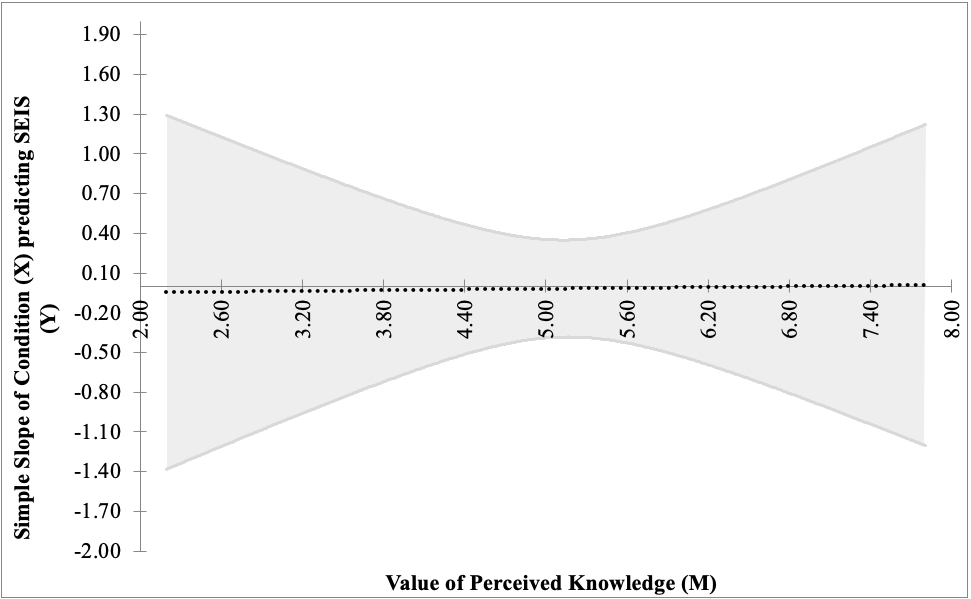
\includegraphics[scale=.40]{Fig5-1.png}
    \caption{Values of the regression coefficient of class predicting support for economic inequality at different levels of perceived knowledge of the causes of human behaviour.}
    \label{fig:twelvthfig}
  \end{center}
\end{figure}

\subsubsection{Exploratory Analyses.}

In exploring my preregistered hypotheses, I did not find any evidence that taking Introduction to Social Psychology (vs. other classes) for a semester led to changing attributions for poverty, or support for economic inequality and redistribution. However, I did observe a pattern of attitude change over the semester in all students (e.g., Table \ref{tab:tenthtable}). Specifically, students in all classes appeared to report more situational, but neither less dispositional attributions for poverty nor less support for economic inequality from Time 1 to Time 2. I explored this observation by conducting a series of two-tailed one-sample t-tests in the entire Time 2 sample. I found that, over the course of the semester, participants reported more situational (\textit{t}(119) = -3.13, \textit{p} = .002, 95\% CI [-.21, -.05]), but not less dispositional (\textit{t}(119) = -.51, \textit{p} = .61, 95\% CI [-.09, .05]) .\footnote{I conducted this test with the Nickols and Nielsen~\cite{nickols11} measure of attributions. The results do not change when analyzing the Guimond, Begin, and Palmer~\cite{guimond89} measure: situational attributions for poverty: \textit{t}(119) = -2.03, \textit{p} = .04, 95\% CI [-.21, -.003]; dispositional attributions for poverty: \textit{t}(119) = .30, \textit{p} = .76, 95\% CI [-.10, .14].} Additionally, students overall did not appear to display diminished support for economic inequality (\textit{t}(117) = -.03, \textit{p} = .98, 95\% CI [-.12, .11]) over the course of the semester.

Given that situational attributions for poverty decreased over the course of the semester I ran a regression to explore whether change in situational attributions for poverty (defined as Time 2 minus Time 1) predicted change in support for economic inequality. I found that increasing situational attributions for poverty did not predict decreasing support for economic inequality ($\beta$ = -.24, \textit{p} = .06). This relationship did not change when I controlled for changes in the perceived knowledge of the causes of human behaviour ($\beta$ = -.23, \textit{p} = .07). It is worth noting, however, that the sample size in these exploratory analyses was only between 115 and 120. These findings suggest that while learning about psychology at the college level may increase awareness of (at least) the situational causes of poverty, this shift does not appear strong enough to influence downstream psychological attitudes such as support for economic inequality. I will caution, however, that these analyses were both exploratory and underpowered. Moreover, they do not allow me to rule out the possible effects of simply passing time, world events, etc. Thus, this is a question that requires further exploration.

\section{General Discussion}

In Chapter 5 I explored whether a semester long introductory social psychology course (versus other psychology courses) that focused heavily on the power of the situation as a determinant of human behaviour influenced attributions for poverty and support for economic inequality. I found that students who took Introduction to Social Psychology did not report higher situational, or lower dispositional attributions for poverty. In addition, students who took Introduction to Social Psychology did not report lower support for inequality or more support for redistribution. This does not mean, however, that a broad education in the situational causes of behaviour has no effect on support for economic inequality. Rather, I found that there was no shift in attributions for poverty and thus the independent variable here was unsuccessful.

The results of Study 5 may suggest that the specificity of the manipulations (i.e., learning about poverty specific causal attributions) in Chapters 3 and 4 are crucial. Instead, learning about the power of the situation must be rooted in educating people to the causes of poverty specifically. Recent research has demonstrated that there is a strong tendency for people to not attend to other people’s ‘headwinds and tailwinds’—the environmental factors that, in part, determine their station in life~\cite{davidai16}. The data presented in this chapter, while not completely comprehensive, suggest that simply educating people about headwinds and tailwinds broadly does not foster more action aimed at addressing economic inequality and poverty more broadly.

Study 6 was novel in that I utilized a field study approach in an attempt to explore how learning about causal attributions in a natural setting might influence attributions for poverty. There were, however, significant limitations that limit the conclusions I can safely draw from Study 6. Primarily, the limitations are centered around methodological challenges. For example, there was a large rate of dropout between the beginning and end of the semester, with 54\% of participants failing to complete the second survey. Additionally, this exploration was only a quasi-experiment; I did not randomly assign people to take different classes. One could also argue that other psychology courses was not the best control. For example, it is possible that “the power of the situation” was conveyed effectively in these other courses as students learned generally about drivers of human behaviour, albeit not as explicitly as within social psychology. A potentially more appropriate control condition would have been seeking participants in classes outside of psychology (e.g., Geography;~\cite{shariff14}), where human behaviour was not emphasized at all.

Given these limitations, the question of whether learning about the causes of general behavior can influence attitudes towards a specific behaviour, or larger societal system, is deserving of further attention. In future experiments, I would like to conduct a more tightly controlled, experimental test of this hypothesis. For instance, randomly assigning participants to read a vignette that clearly describes the myriad situational and dispositional causes of others behaviour generally versus a vignette that describes only the dispositional causes of behaviour. Another example might be to educate participates on the headwinds and tailwinds that underlie many behaviours and outcomes~\cite{davidai16} and then measure shifts in specific attributions, such as attributions for poverty, and subsequent attitudes towards larger societal issues such as economic inequality.

	Shedding further light on this topic is crucial for understanding how to plan potential interventions. As the results of earlier chapters suggest, it may be beneficial to design attitude-specific interventions such as poverty simulations or cross-SES interaction. However, understanding more clearly the specificity of these effects could allow for the development of more broadly applicable, and far reaching, interventions. For example, would it be possible to design and implement a more general intervention targeting the understanding of headwinds and tailwinds, broadly, in order to foster more tolerance, or do these interventions need to be specific to a particular attitude? The results of the Study 6 suggest that specificity might be key—that general interventions would not be as useful as direct, targeted interventions. However, more research is needed to address the methodological limitations of this Study.   
\chapter{General Discussion}

Economic inequality is a major threat to social cohesion (e.g.,~\cite{kawachi97, lichbach89}), health~\cite{wilkinson06}, and political stability (e.g.,~\cite{murphy01}). Yet, people in North America remain relatively apathetic towards inequality, especially in comparison to far less directly threatening issues such as terrorism and illegal immigration~\cite{mccarthy16}. In this dissertation I sought to explore one potential underlying cause of this relative apathy. Specifically, I examined the relationship between attributions for poverty and downstream psychological attitudes, such as support for economic inequality, support for wealth redistribution, as well as direct helping behaviour aimed at the poor.

\section{Summary of Results}
\subsection{Are Dispositional Attributions for Poverty Associated with Support for Economic Inequality?}

I began this dissertation by exploring the link between attributions for poverty and support for economic inequality. Past studies have shown that North Americans favour dispositional attributions for others’ behaviour in general~\cite{bem72, jones65} and specifically when explaining the causes of poverty (e.g.,~\cite{cozzarelli01, feagin75, feather74, halpern93}. However, few had explored how attributional style relates to other political beliefs and the studies that had were limited in scope (e.g., North America) and sample (most sample sizes below 200). Thus, my first goal was to cross-nationally test this relationship using a large data set of over 30,000 observations across 34 countries. Across these data, participants indicated whether they believed that poverty was due primarily to (a) dispositions, such as laziness, or (b) situations, such as an unfair society, as well as the degree to which they thought that that incomes should be made more or less equal. Consistent with previous work, I found that across the globe people who endorsed more situational attributions for poverty were less tolerant of economic inequality. This finding held when controlling for both individual (e.g., age, political orientation) as well as country-level covariates (e.g., GDP per capita, actual economic inequality). Thus, Study 1 of this dissertation provides a large-scale cross-national replication of the finding that attributions for poverty may indeed play a role in the relative apathy towards economic inequality that exists in North America.

\subsection{Are Attributions for Poverty Malleable, and can they be Altered to Decrease Support for Economic Inequality?}

In Chapter 2 I demonstrated, with a large cross-national sample, that situational and dispositional attributions for poverty are linked to support for economic inequality. In the following two chapters I sought to build upon these findings. First, I examined whether perspective taking (Chapter 3) and stereotype disconfirmation via cross-SES contact (Chapter 4) can shift situational and dispositional attributions for poverty. Second, I aimed to investigate whether attributions for poverty are causally linked to support for economic inequality and redistribution.

\subsubsection{Perspective Taking.}

In Chapter 3 I explored the utility of a short and immersive perspective taking task as a route to shifting attributions for poverty and support for economic inequality. Study 2a was a small-scale pilot study in which participants came into the lab and were randomly assigned to spend approximately ten minutes playing either a short, but immersive, online poverty simulation called SPENT or an online version of Monopoly. Following this task, participants completed a survey containing measures of attributions for poverty, support for economic inequality, and support for redistribution. I found that after engaging in the poverty simulation (versus a game of Monopoly) participants demonstrated less dispositional, and more situational, attributions for poverty. This change, in turn, led participants to report less support for economic inequality but no change in support for wealth redistribution. As such, Study 2a provided initial evidence that attributions for poverty can be shifted via perspective taking, and that there is a causal relationship between attributions for poverty and support for economic inequality. However, this study had several limitations. For instance, the sample size was relatively small, which may have made a few key effects difficult to detect (e.g., the effect of SPENT on support for economic inequality). Additionally, the control condition was not optimal; it is possible that playing Monopoly could have primed thoughts of wealth or identification with the wealthy. In addition, I also wondered if the observed effects might persist once participants leave the lab. Thus, I conducted Study 2b, a high-powered pre-registered replication of Study 2a.
	
In Study 2b participants came into the lab and were randomly assigned to either play SPENT or complete a no-game control condition in which they simply filled out the same survey as Study 2a without playing any game. Once again, I found that participants who engaged in SPENT (versus a no-game control condition) reported higher situational attributions for poverty as well as lower support for inequality and increased support for wealth redistribution. Counter to the findings of Study 2a, however, it appears that with a stronger, higher powered design SPENT primarily affected situational attributions for poverty (there was no significant change in dispositional attributions for poverty). This finding bore out in mediation analyses as well, showing a significant indirect effect of playing SPENT through situational, but not dispositional, attributions for poverty. These null effects on dispositional attributions for poverty makes sense post-hoc, given that SPENT is largely focused on informing the player of the myriad uncontrollable situations that can befall individuals living in poverty.
	
In addition to replicating the key findings of Study 2a, in Study 2b I explored whether these effects persist beyond immediate assessment in the lab by measuring attributions for poverty and support for economic inequality one day after study participation and, on average, five months later. First, I found that when asked one day later, participants who played SPENT still reported higher situational attributions for poverty and diminished support for economic inequality. Moreover, two of the three original effects were detectable at the end of the semester, an average of 155 days after the initial study; participants who played SPENT, relative to a no-game control condition, reported higher situational attributions for poverty and lower support for economic inequality. 

\subsubsection{Stereotype Disconfirmation and Cross-SES contact.}

In Chapter 4, I explored the psychological consequences of presenting poverty stereotype disconfirming evidence through two cross-SES contact studies. In Study 3a participants came into the lab believing they were participating in a study in which they would have a one-on-one conversation with another psychology student. In reality, the second participant was a confederate randomly assigned to act as either an average-SES or low-SES person. Specifically, the confederate gave a cue during an iteration of the fast-friends paradigm indicating they were either financially sound or struggling. Importantly, in both conditions the confederate gave additional cues demonstrating they work hard to counter the stereotype that the poor are lazy. Following this, participants completed the same questionnaire as in Chapter 2 containing measures of attributions for poverty, support for economic inequality, and support for redistribution. Most findings in Study 3a were null; I did not find any difference in attributions for poverty, support for economic inequality, or redistribution between the low and average-SES conditions. There were, however, several limitations in Study 3a. Specifically, the manipulation may have been too subtle and the sample size too small to detect the size of effect I was seeing. Therefore, I conducted Study 3b to address these limitations and explore more thoroughly how cross-SES may shift attributions for poverty and support for economic inequality.

In Study 3b a larger sample of participants engaged in the same one-on-one fast friends interaction as Study 3a, with three key differences. First, the confederate referenced their own SES at two separate occasions during the interaction to increase the salience of this information. Second, the confederate wore a sweater consistent with their SES: a brand-new sweater in the average-SES condition compared with a tattered version of the same sweater in the low-SES condition. We added the sweaters in order to convey SES with a separate, potentially more salient, cue. Lastly, I included a direct measure of helping in which participants were given the chance to donate raffle tickets for a \$100 cash draw directly to their conversation partner via an anonymous dictator game. Using the stronger and more adequately powered design in Study 3b, I found that a simple cross-SES interaction led to lower dispositional attributions for poverty, but no difference in situational attributions for poverty across conditions. This suggests that a cross-SES interaction can successfully dispel the stereotype that the poor are lazy. While there was no difference in support for economic inequality or redistribution across conditions, the cross-SES interaction led to significantly higher levels of aid, as captured in the dictator game, toward conversation partner. However, in Study 3b I did find a significant indirect effect of dispositional attributions for poverty mediating the relationship between the cross-SES interaction and support for economic inequality.

\subsection{Is the Relationship Between Causal Attributions and Support for Economic Inequality Poverty-Specific?}

In Chapters 3 and 4 I found that increasing situational and decreasing dispositional attributions for poverty can have demonstrable downstream effects on support for economic inequality as well as specific, targeted helping behaviour. One lingering question, however, was whether educating people about the situational forces that frequently shape human behaviour in daily life may have a similar impact on reducing support for economic inequality and helping the poor. In Chapter 5, I explored this question using a field quasi-experiment.

Across two semesters, I recruited students from various second year psychology classes. Specifically, I recruited students from an Introduction to Social Psychology wherein students learned extensively about one particular course theme—the power of the situation. This theme was not tied directly to poverty, but instead simply highlighted how situational factors can exert strong influence on nearly every aspect of our lives. Comparatively, students in the other classes did not have this same emphasis on the power of the situation. At both the beginning and end of the semester, all of the participants completed the same key measures as the previous chapters: attributions for poverty, support for economic inequality, and support for redistribution.

Due to generally low recruitment at the beginning of the semester, Study 4 was relatively underpowered. Regardless, I did not find any significant differences on the key dependent variables between participants in social psychology and participants in the other introductory psychology classes. Learning about the power of the situation via a semester long social psychology class did not appear to increase situational attributions for poverty or decrease dispositional attributions for poverty. Additionally, neither support for economic inequality nor redistribution appeared to shift throughout the semester or between people who took Introduction to Social Psychology and the control classes. While these findings are ultimately difficult to interpret, these data suggest it is worth exploring this question more thoroughly in the future.

\section{Implications}

Classic research in Social Psychology has revealed that people in North America tend to view another person’s actions or behaviour as a result of their disposition or internal nature (as opposed to their response to situational cues;~\cite{gilbert95}). Can these attributions be altered? Might shifting situational/dispositional attributions for poverty impact attitudes towards economic inequality? My dissertation presents six studies to unpack these research questions.

\subsection{Theoretical Implications}

There is a significant body of work exploring how we make attributions for behaviour, a smaller body of research exploring attributions for poverty specifically, and a non-existent body of literature exploring the causal relationship between attributions for poverty and various psychological attitudes and behaviour aimed towards people who live in poverty. The work presented in this dissertation falls primarily in the latter two categories.

First, Chapter 2 served as a large-scale conceptual replication of the finding that attributions for poverty are related to other psychological attitudes. Past research has shown that there are some links between attributions for poverty and attitudes and behavior aimed directly at the poor~\cite{bullock03, cozzarelli01, zucker93}. I expand on this body of work in two ways. First, the past studies that have explored these relationships have all been very small (e.g., ns < 200), correlational studies in specific (e.g., American) samples. Chapter 2 of this dissertation demonstrates, with a large cross-national sample spanning 34 countries, that attributional style (i.e., primarily dispositional or situational attributions) in the context of poverty does indeed bear on other related psychological attitudes. Secondly, and more critically, Chapter 2 shows that attributions for poverty bear on psychological attitudes that are not necessarily aimed directly at the poor. That is, previous work has shown that attributions for poverty can affect specific target-specific attitudes such as blame and anger directed specifically at the poor. I extend this work by demonstrating that attributions for poverty can influence the way we feel about larger societal structures, particularly the justness of economic inequality. This is crucial in showing that these somewhat culturally determined attributional styles can potentially influence important social outcomes, like voting on particular political policies such as social programs.

Second, the studies presented in Chapters 3 through 5 are the first, to my knowledge, to experimentally test the link between attributions for poverty and other attitudes and behaviours, such as support for economic inequality and willingness to help the poor. While previous research has demonstrated that the link is there, my work demonstrates that both (a) attributions are to some extent malleable, and (b) shifting attributions can causally impact the way one things about, and behaves towards, people who live in poverty. That being said, attribution theory is very nuanced, and my work primarily fits in one small corner therein.

Specifically, Weiner~\cite{weiner85} proposed that there are three dimensions to causal inference: locus, controllability, and stability. I have situated the entirety of this work under the umbrella of locus—is poverty caused by factors internal or external to the person? This focus does not consider other elements of Weiner’s~\cite{weiner85} model. For example, would we observe similar findings that making people aware of the situational causes of poverty can shift support for economic inequality if we additionally describe poverty as also controllable versus uncontrollable? Does support for economic inequality shift when we make participants aware of the situational causes of poverty but also vary perceptions of poverty as (un)controllable or (un)stable? On the whole, attribution theory in its current state puts forth a nuanced view of how we understand the causes of behaviour and the work presented here is focused almost entirely on only one of those dimensions.
	
One potential future avenue I would like to explore is perceptions of poverty and wealth over the life course—that is, the instability of the socioeconomic system. While researchers and laymen alike tend to think of poverty or wealth as static life outcomes—either you end up poor or rich. However, recent research has shown that social class is a far more dynamic and fluid process. For example, over the course of a lifetime approximately 42\% of people will experience at least one year in the bottom 10\% of earners\cite{rank15}, and approximately 11\% of people will experience at least one year in the top 1\% of earners\cite{hirschl15}. I would predict that given information on the relative instability of poverty and wealth people may demonstrate more support for inequality and less support for redistribution. It is possible that if socioeconomic status is seen as unstable, people are likely to fall or rise to their deserved position. Additionally, the dimensions proposed by Weiner~\cite{weiner85} likely interact; for example, being told that poverty and wealth are controllable and unstable could possibly dampen the effects of simply learning that there are uncontrollable situational causes to obtained social status.

Lastly, one of crucial theoretical contributions of the present work is the evidence that, in line with past work on causal attributions more broadly, attributions for poverty, while related, are not necessarily hydraulic in nature. That is, in the present work dampening perceptions of the situational causes of poverty did not necessarily correspond to a boost in perceptions of the dispositional causes of poverty. Intuitively, attributions seem to be a construct that exists on a continuum, so by definition an increase in one would necessitate a decrease in the other. Past theorizers have argued, though, that situational and dispositional attributions may be orthogonal~\cite{kluegel86}. Some past research has supported this idea with correlational evidence, showing that situational and dispositional attributions for behaviour are uncorrelated~\cite{taylor76, miller81} as opposed to negatively correlated as you might expect if they were not orthogonal. In the present work, Studies 2b and 3b provide causal evidence for orthogonality. When situational attributions for poverty were highlighted via a poverty simulation I found that situational attributions went up whereas dispositional attributions did not change. Conversely, when dispositional attributions were highlighted via an instance of cross-socioeconomic contact dispositional attributions went up whereas situational attributions remained unchanged. Thus, I add to the body of literature supporting the orthogonality of causal attributions, specifically in the context of poverty, with an experimental demonstration that shifting one need not translate into a complementary shift in the other. Future research should explore the relative efficiency of addressing social woes, such as support for economic inequality via one pathway or the other; which is more effective, impactful, and practical?

\subsection{Practical Implications}

Support for policies aimed at addressing poverty and economic inequality (e.g., support for redistribution) has not increased over the last five decades, despite large increases in inequality~\cite{ashok15}. One possible reason for this lack of support is a misunderstanding surrounding the causes of poverty. The data presented in this dissertation suggest that the introduction of data-based interventions, such as immersive perspective taking exercises, could increase understanding of some of the situational causes of poverty. In turn, a greater appreciation of the situational factors leading to poverty may bolster support for economic policies that assist people living in poverty and address some of the systemic factors that contribute to maintaining poverty and inequality (e.g., banning of predatory payday lending practices). Of course, large-scale attitude change is a difficult task. This is not to suggest that, for instance, a poverty simulation is a perfect remedy for relative apathy towards economic inequality. Instead, I propose that understanding how attributions for poverty may influence support for economic inequality is a good starting point for designing meaningful and impactful interventions.

One such promising intervention, as outlined in Chapter 3, is a poverty simulation. The data suggests that the SPENT game can have a significant and meaningful impact on causal attributions and attitudes towards economic inequality, both immediately and at an extensive delay, and thus the game itself may be used as an intervention tool. Some organizations (e.g., \href{http://www.makethemonth.ca/}{The United Way of the Lower Mainland}) currently use similar, if not more impactful, iterations of this idea through poverty simulations in which participants are challenged with surviving a simulated month on wages below the local poverty line. Particularly, the Missouri Community Action Network has developed and oversees an immersive poverty simulation that is run across North America. I have not come across any systematic testing of these large-scale poverty simulations, and thus this is an excellent avenue for future research on the potential utility of this intervention. The data I presented in Chapter 3 shows that there is promise in a large-scale intervention such as this, but further testing to truly understand the efficacy is needed. The challenge with implementing interventions such as poverty simulations in the world, though, is that they suffer from self-selection biases; people who participate are people who have chosen to participate and are thus, at least in some minor capacity, interested in understanding poverty more deeply. Thus, it may be beneficial to explore the feasibility of implanting poverty simulations into educational curricula. The SPENT game, while not yet tested on a large scale, offers potential in this regard due to its short, free-to-use nature.
	
Strong instances of stereotype disconfirmation also may be an effective tool at changing attributions for poverty, and thus can also be leveraged to foster change in societal perceptions of poverty and willingness to help the poor. While far more work is required to evaluate the utility of interventions such as these, the data presented in Chapter 4 of this dissertation suggest that interventions aimed at increasing exposure to, or awareness of, the hardworking poor may be beneficial for fostering warmer attitudes towards the poor. There is some evidence that exposure to poverty can increase willingness to help the poor (e.g.,~\cite{piff10}). However, this work focused on lower class individuals. Contrary to this, a large field experiment with upper class people demonstrated that simple exposure to poverty actually decreased willingness to help the poor~\cite{sands17}. Simple exposure to poverty is not enough to motivate helping behaviour, thus the present work suggests that exposure to hardworking poor specifically may be a fruitful avenue for attitude and behaviour change.

\section{Limitations}

One large and overarching limitation present across many of the studies in this dissertation is the over-reliance on readily available (Canadian) undergraduate samples. This reality presents a unique challenge for two reasons. First, reliance on undergraduate samples may mean that participants are in lower income brackets. Additionally, with respect to socioeconomic status students can be an atypical group in that they are personally of low income but are still supported by their parents, thus making socioeconomic status information difficult to attain. The reason the reliance on students was problematic can be seen most clearly in Chapter 4. In the initial exploration of cross-SES contact I found that many of my participants were already of low income and thus the contact was, by definition, not cross-SES. When attempting to evaluate attributions for those who live in poverty one can imagine that the group themselves will make different attributions compared with people who are not living in poverty. Second, I collected all of the data for this dissertation (except for Chapter 2) in a country where there is strong support for a wider social safety net. It may be beneficial, then, to attempt to replicate these findings in a population that is (a) higher income, and (b) from a country (e.g., the United States) that focuses more predominantly on dispositional attributions for poverty.

In addition to the focus on Canadian samples, the present research is highly focused on poverty as both a consequence of, and route to alleviating, economic inequality. Specifically, I have focused on manipulating understanding of the causes of poverty, as well as addressing poverty as viable route to addressing economic inequality (e.g., support for redistribution, willingness to help the ostensibly poor confederate). Inequality, however, need not be tied exclusively to poverty. Additionally, it is possible that learning about the situational causes of poverty may push people towards a willingness to address economic inequality simply as a means to alleviate poverty that is seen as unfair. Thus, in future research I would like to explore support for economic inequality in a context that is removed from specifically attributions for poverty. For instance, if we made people aware instead of situational causes of wealth will they also demonstrate less support for economic inequality? 

Another potential concern is the use of small sample sizes for some of the experiments in Chapters 3 through 5. This issue was primarily due to the fact that recruitment for these experiments, as well as the logistics of running these experiments (particularly those in Chapter 4), was quite time consuming and difficult. I attempted to address this issue where possible (e.g., in Study 3b), however it was not possible in some cases. For instance, Study 3b required significant research assistant time and coordination and I was therefore unable to collect a larger sample. However, I addressed this limitation in Study 2b with the utilization of a sequential design that should have alleviated some of these concerns. Additionally, my inability to leverage larger sums of money to pay participants was partially the cause of these small samples, particularly in my longitudinal explorations. For instance, in Study 4 I was only able to offer a total of \$500 in prizes to participants. With that, it was difficult to strongly incentivize participation across the semester. This issue was also present with Study 2b, in which I was only able to offer one small prize for participants to complete a third (and unexpected) survey. The implications of this limitation are two-fold. First, it is difficult to interpret the null effects of Study 4, and second, the conclusions of Study 2b are tentative. However, these results are nonetheless promising.

Finally, one methodological limitation present in this dissertation was a flawed (in hindsight) decision regarding one of the measures I chose to include in Studies 2b and 3b. I conducted Studies 2a and 3a concurrently and within each study I utilized two separate measures of attributions for poverty. In both studies, I observed larger effects of the manipulation on the Nickols and Nielsen~\cite{nickols11} measure as opposed to the Guimond et al.,~\cite{guimond89} measure. Given that the Nickols and Nielsen~\cite{nickols11} measure appeared more responsive to the manipulation, and Studies 2b and 3b would contain almost identical manipulations, I opted to only include the Nickols and Nielsen~\cite{nickols11} measure in these studies. However, following data collection for these studies I computed scale reliabilities, as well as factor analyzed, both scales in response to a reviewer pointing out that the Guimond et al.,~\cite{guimond89} measure appeared more face valid. In these analyses I discovered that not only is the Guimond et al.,~\cite{guimond89} measure far more internally consistent, but a linear factor analyses revealed two clean, distinct factors that align perfectly with the way the original authors defined the scale. On the other hand, the linear factor analysis of the Nickols and Nielsen~\cite{nickols11} measure revealed a very messy and overlapping set of two factors with some items loading equally on both factors. This methodological limitation applies to Studies 2b and 3b. While I don’t believe it undermines the conclusions due to the similar effect sizes and results across both measures in Studies 2a and 3a, Studies 2b and 3b would have been stronger had I chosen the Guimond et al.,~\cite{nickols11} measure. Future studies should use primarily this measure when assessing attributions for poverty.

\section{Future Directions}

One of the most interesting findings of this dissertation is that participating in a single short online poverty simulation can impact perceptions of the causes of poverty, support for economic inequality, and views on redistribution up to five months later. The initial one-day follow-up in Study 3b was planned, however the second long-term follow-up was an instance of opportunistic data collection that was not pre-planned or pre-registered in any way except for the fact that the main analyses remained the same. One area of future research I would like to explore is the robustness of these effects in an experiment that is deliberately planned to be a longitudinal study. For example, a study in which participants are informed from the beginning that participation will be a six month to one-year commitment with surveys at three-month intervals. This would allow a large enough time gap to avoid possible practice effects of participants completing the same measures repeatedly. Additionally, having a study planned this way would likely reduce attrition to a more manageable proportion and initial sample size can be planned around expecting attrition at the one-year point. A study such as this is crucial determining whether the effects of a short poverty simulation will reliably hold over time.

As noted in the theoretical implications, there are many possible boundary conditions to understanding how and when manipulations of attributions may work and be more or less effective. For instance, does engaging in an online or in-person poverty simulation influence donation behaviour in response to an unrelated donation or petition signature solicitation at a later date? Another critical moderator to the effectiveness of these interventions may be when, and to whom, these manipulations are presented. For instance, one worthwhile endeavour would be to explore whether the effects observed in Chapters 3 and 4 could be amplified if administered at critical stages in development (e.g., during high school or early formative college years). Past research shows that personality development tends to stabilize by the time a person is approaching their late 20s~\cite{costa94, specht11}. While the present research was conducted primarily with college-age students, it would be informative to explore these interventions both earlier and later in lifespan development. Specifically, I suspect that interventions such as a poverty simulation would affect more long-lasting change in adolescents, and less in older adults.

I would also like to conduct a stronger test of the hypothesis that shifting broad causal attributions can impact support for economic inequality. Study 4 quasi-experimentally demonstrated that spending a full semester learning about the situational causes of behaviour did not impact attributions for poverty or support for economic inequality and redistribution. However, some of my additional research lends support that a more general understanding of the causes of behaviour can influence support for economic inequality. For example, my colleagues and I found some mixed evidence that when people more strongly believe in free will they are more supportive of economic inequality~\cite{mercierunpub}. One possible way of testing this question more directly would be randomly assigning people to read a target article that convincingly describes myriad situational factors that can influence behaviour and outcomes, alongside internal factors (e.g., hard work, free will) versus a control article. Then, following this more general manipulation of attributions for behaviour measuring change in attributions for specific behaviours and outcomes (e.g., poverty, professional success, personal happiness, etc.). A series of experiments along this line is crucial for understanding the specificity of these effects; can we change attributions for specific behaviors with general interventions, or must the interventions be behaviour specific?

As the work in this dissertation shows, people have biased perceptions of poverty which, to some extent, impacts the way they people interact with the poor. Human judgment is susceptible to biases and skewed perceptions in many domains—cognitive errors such as the correspondence bias or other heuristics are commonplace. Thus, one crucial future direction I would like to explore is how other heuristics and cognitive errors (e.g., the availability or representativeness heuristic) may stifle progress towards a generally more tolerant society. One specific case I would like to explore is potentially biased views of welfare spending in the United States. Unlike the literature on attributions for poverty, there is minimal past research exploring what Americans see and understand about welfare spending. For example, one past analysis shows that from 1938 to 1995, the majority of survey respondents in a large public opinion poll simultaneously believed that the government should do more to help those in need and should spend less on welfare~\cite{macleod99}. Additionally, one previous study demonstrated a bias in the understanding of welfare spending; nearly one-quarter of participants thought that U.S. Federal welfare spending was more than 20\% of the national budget (the actual amount was 8.2\%) and that the average welfare recipient was young, non-white, and female~\cite{sotirovic01}. In the future, I would like to conduct extensions of this work in which I examine whether it is possible to correct for these, and other, biases of social welfare and explore the downstream psychological effects. For example, in future experiments I would like to present participants with actual rates of welfare spending (versus the perceived rates, as determined by a pilot study) to examine whether welfare spending is significantly lower than the public perception. Then, it will be possible to see if understanding how much resources are being allocated to helping the poor people will be more open to this as a tool for addressing inequality via poverty. Additionally, given some research demonstrates incorrect racial biases in perceived welfare spending~\cite{sotirovic01}, it might be possible to shift support for inequality and redistribution by addressing larger issues such as racism and xenophobia, perhaps via perspective taking exercises akin to Studies 2a and 2b. 

\section{Conclusion}

Fostering attitude or behaviour change begins with understanding the root of the underlying attitudes~\cite{weiner85}. In the present work I have found evidence that a general predisposition to internal attributions for economic outcomes such as poverty in part underlies support for economic inequality. By placing the blame of poverty squarely on the shoulders of the poor, people may feel justified in saying ‘pull yourself up by the bootstraps!’ and declaring that they have done their part to address poverty. This perspective may be comforting insofar as it allows one to maintain a comfortable belief that people rise and fall to the economic station they deserve. However, it overlooks a potentially large and influential cause of poverty—systemic, institutional, and uncontrollable external factors—and may stall action aimed at addressing inequality. The work presented here demonstrates that shifting attributions for poverty can impact attitudes towards the poor and thus support for economic inequality. By understanding some avenues towards shifting attributions for poverty, we can then begin to address the root causes of these attitudes and produce a more tolerant society. 


%   BACK MATTER  %%%%%%%%%%%%%%%%%%%%%%%%%%%%%%%%%%%%%%%%%%%%%%%%%%%%%%%%%%%%%%
%
%   References and appendices. Appendices come after the bibliography and
%   should be in the order that they are referred to in the text.
%
%   If you include figures, etc. in an appendix, be sure to use
%
%       \caption[]{...}
%
%   to make sure they are not listed in the List of Figures.
%

\backmatter%
	\addtoToC{Bibliography}
	\bibliographystyle{plain}
	\bibliography{references}
	
\end{document}
